\documentclass[whitelogo]{tudelft-report}

% Packages
\usepackage{natbib}
\usepackage{changes}
\usepackage{hyperref}
\usepackage{graphicx}
\usepackage{float}
\usepackage{xcolor, color,soul}
\usepackage{amsmath}
\usepackage{subcaption}
\usepackage{amssymb}
\usepackage{amsthm}
\usepackage{extarrows}
\usepackage{csquotes}
\usepackage[utf8]{inputenc}
\usepackage[T1]{fontenc}
\usepackage{mathtools}
\usepackage{qcircuit}
\usepackage{optidef}
\usepackage{abstract}
\usepackage{etoolbox}
\usepackage{caption}
\usepackage{bm}
\usepackage{doi}

\DeclareMathAlphabet{\mathcal}{OMS}{cmsy}{m}{n}

\patchcmd{\abstract}{\null\vfil}{}{}{}

% Commands
\renewcommand{\vec}[1]{\bm{#1}}
\newcommand{\drawline}{\rule{4.5in}{.4mm}}
\newcommand{\define}{:=}
\newcommand{\gambe}{\vec{\gamma},\vec{\beta}}
\newcommand{\prob}[1]{\text{Pr}[#1]}
\newcommand{\expect}[1]{\text{E}[#1]}
\newcommand{\myeq}[1]{\stackrel{\mathclap{\normalfont\mbox{#1}}}{=}}
\newcommand{\diag}[1]{\text{diag}\{#1\}}
\newcommand{\CNOT}{\text{CNOT}}
\newcommand*\diff{\mathop{}\!\mathrm{d}}
\def\code#1{\texttt{#1}}

% Lemmas, definitions, theorems
\newtheorem{lemma}{Lemma}[section]
\newtheorem{theorem}{Theorem}[section]
\theoremstyle{definition}
\newtheorem{definition}{Definition}[section]
\newtheorem*{remark}{Remark}

\begin{document}

%% Use Roman numerals for the page numbers of the title pages and table of
%% contents.
\frontmatter

%% Uncomment following 19 lines for a cover with a picture on the lower half only
%\title[tudelft-white]{Title}
%\subtitle[tudelft-cyan]{Optional subtitle}
%\author[tudelft-white]{J.\ Random Author}
%\affiliation{Technische Universiteit Delft}
%\coverimage{cover.jpg}
%\titleoffsetx{10cm}
%\titleoffsety{10cm}
%\afiloffsetx{1cm}
%\afiloffsety{18cm}
%\covertext[tudelft-white]{
%    \textbf{Cover Text} \\
%    possibly \\
%    spanning 
%    multiple 
%    lines
%    \vfill
%    ISBN 000-00-0000-000-0
%}
%\makecover

%% Uncomment following 16 lines for a cover with a picture on the lower half only
\title[tudelft-white]{The Quantum Approximate Optimization Algorithm} %Title
\subtitle[tudelft-black]{Performance on Max-Cut \\using Heuristic Parameter determination} % Subtitle
\author[tudelft-white]{J.C.P. Bus}
\affiliation{Technische Universiteit Delft}
%\coverimage{figures/cover/quantum-machinery-microsoft.png} % AANPASSEN
%\covertext[tudelft-white]{
%    \textbf{Cover Text} \\
%    possibly \\
%    spanning 
%    multiple 
%    lines
%    \vfill
%}
\setpagecolor{tudelft-cyan}
\makecover[split]


%% Include an optional title page.
\begin{titlepage}


\begin{center}

%% Insert the TU Delft logo at the bottom of the page.

%% Print the title in cyan.
{\makeatletter
\largetitlestyle\fontsize{64}{94}\selectfont\@title
%\largetitlestyle\color{tudelft-cyan}\Huge\@title
\makeatother}

%% Print the optional subtitle in black.
{\makeatletter
\ifx\@subtitle\undefined\else
    \bigskip
   {\tudsffamily\fontsize{22}{32}\selectfont\@subtitle}    
    %\titlefont\titleshape\LARGE\@subtitle
\fi
\makeatother}

\bigskip
\bigskip

by
%door

\bigskip
\bigskip

%% Print the name of the author.
{\makeatletter
%\largetitlefont\Large\bfseries\@author
\largetitlestyle\fontsize{26}{26}\selectfont\@author
\makeatother}

\bigskip
\bigskip

to obtain the degree of Bachelor of Science
%ter verkrijging van de graad van Master of Science

at the Delft University of Technology,
%aan de Technische Universiteit Delft,

to be defended on Thursday, 23 July 2020 at 10:00.
%in het openbaar de verdedigen op dinsdag 1 januari om 10:00 uur.

\vfill

\begin{tabular}{lll}
    Student number: & 4553896 \\
    Project duration: & \multicolumn{2}{l}{January, 2020 -- July, 2020} \\
    Thesis committee: & Dr.\ C. Garc\'ia Almudever, & TU Delft, supervisor \\
        & Dr.\ M. M\"oller, & TU Delft, supervisor \\
        & Dr. ir. \ L.J.J. van Iersel, & TU Delft \\
        & Dr. ir.\ M. Veldhorst, & TU Delft \\
        & Dr. \ M. Wimmer, & TU Delft
\end{tabular}
%% Only include the following lines if confidentiality is applicable.

\bigskip
\bigskip
%\emph{This thesis is confidential and cannot be made public until December 31, 2013.}
%\emph{Op dit verslag is geheimhouding van toepassing tot en met 31 december 2013.}

\bigskip
\bigskip
An electronic version of this thesis is available at \url{http://repository.tudelft.nl/}.
%\\[1cm]

%\centering{
\includegraphics{cover/logo_black}}


\end{center}

\begin{tikzpicture}[remember picture, overlay]
    \node at (current page.south)[anchor=south,inner sep=0pt]{
        
\includegraphics{cover/logo_black}
    };
\end{tikzpicture}

\end{titlepage}



\chapter*{Preface}
\setheader{Preface}

Preface\ldots

\begin{flushright}
{\makeatletter\itshape
    \@author \\
    Delft, January 2013
\makeatother}
\end{flushright}



\tableofcontents

%% Use Arabic numerals for the page numbers of the chapters.
\mainmatter

\chapter{Introduction}

This document is intended to be both an example of the TU Delft \LaTeX{} template for reports and theses, as well as a short introduction to its use. It is not intended to be a general introduction to \LaTeX{} itself,\footnote{We recommend \url{http://en.wikibooks.org/wiki/LaTeX} as a reference and a starting point for new users.} and we will assume the reader to be familiar with the basics of creating and compiling documents.

Instructions on how to use this template under Windows and Linux, and which \LaTeX{} packages are required, can be found in \texttt{README.txt}.

\section{Document Structure}

Since a report, and especially a thesis, might be a substantial document, it is convenient to break it up into smaller pieces. In this template we therefore give every chapter its own file. The chapters (and appendices) are gathered together in \texttt{report.tex}, which is the master file describing the overall structure of the document. \texttt{report.tex} starts with the line
\begin{quote}
    \texttt{\textbackslash documentclass\{tudelft-report\}}
\end{quote}
which loads the TU Delft report template. The template is based on the \LaTeX{} \texttt{book} document class and stored in \texttt{tudelft-report.cls}. The document class accepts several comma-separated options. The default language is English, but this can be changed to Dutch (\emph{e.g.}, for bachelor theses) by specifying the \texttt{dutch} option:
\begin{quote}
    \texttt{\textbackslash documentclass[dutch]\{tudelft-report\}}
\end{quote}
Furthermore, hyperlinks are shown in blue, which is convenient when reader the report on a computer, but can be expensive when printing. They can be turned black with the \texttt{print} option. This will also turn the headers black instead of cyan.

If the document becomes large, it is easy to miss warnings about the layout in the \LaTeX{} output. In order to locate problem areas, add the \texttt{draft} option to the \texttt{\textbackslash documentclass} line. This will display a vertical bar in the margins next to the paragraphs that require attention. Finally, the \texttt{nativefonts} option can be used to override the automatic font selection (see below).

This template has the option to automatically generate a cover page with the \texttt{\textbackslash makecover} command. See the next section for a detailed description.

The contents of the report are included between the \texttt{\textbackslash begin\{document\}} and \texttt{\textbackslash end\{document\}} commands, and split into three parts by
\begin{enumerate}
\item\texttt{\textbackslash frontmatter}, which uses Roman numerals for the page numbers and is used for the title page and the table of contents;
\item\texttt{\textbackslash mainmatter}, which uses Arabic numerals for the page numbers and is the style for the chapters;
\item\texttt{\textbackslash appendix}, which uses letters for the chapter numbers, starting with `A'.
\end{enumerate}
The title page is defined in a separate file, \emph{e.g.}, \texttt{title.tex}, and included verbatim with \texttt{\textbackslash input\{title\}}.\footnote{Note that it is not necessary to specify the file extension.} Additionally, it is possible to include a preface, containing, for example, the acknowledgements. An example can be found in \texttt{preface.tex}. The table of contents is generated automatically with the \texttt{\textbackslash tableofcontents} command. Chapters are included after \texttt{\textbackslash mainmatter} and appendices after \texttt{\textbackslash appendix}. For example, \texttt{\textbackslash input\{chapter-1\}} includes \texttt{chapter-1.tex}, which contains this introduction.

The bibliography, finally, is generated automatically with
\begin{quote}
    \texttt{\textbackslash bibliography\{report\}}
\end{quote}
from \texttt{report.bib}. The bibliography style is specified in \texttt{tudelft-report.bst}, which is a modified version of \texttt{apsrev4-1.bst} (from REVTeX) designed to also display the titles of referenced articles. The template will automatically generate clickable hyperlinks if a URL or DOI (digital object identifier) is present for the reference. As an example, we cite the paper by Nobel laureate Andrei Geim and his pet hamster \citep{Geim2001}. Although it is possible to manage the bibliography by hand, we recommend using EndNote (available from Blackboard) or JabRef (available from \url{http://jabref.sourceforge.net/}).

\section{Cover and Title Page}

This template will automatically generate a cover page if you issue the \texttt{\textbackslash makecover} command. There are two formats for the cover page: one with a page-filling (`bleeding')
illustration, with the title(s) and author(s) in large ultrathin typeface, and the other where the illustration fills the lower half of the A4, whereas title(s), author(s) and additional
text are set in the standard sans-serif font on a plain background with a color chosen by the user. The last option is selected by the optional key \texttt{split}: \texttt{\textbackslash makecover[split]} yields
a page with the illustration on the lower half. All illustrations are bleeding, in accordance with the TU Delft style.

Before generating the cover, you need to provide the information to put on it. This can be done with the following commands:
\begin{itemize}
\item\texttt{\textbackslash title[Optional Color]\{Title\}} \\
    This command is used to provide the title of the document. The title
    title is also printed on the spine. If you use a title page (see below), this information will be used there as well.
    As the title, subtitle and author name are printed directly over the cover photo, it will often be necessary to adjust the print color in order to have
    sufficient contrast between the text and the background. The optional color argument is used for this.
\item\texttt{\textbackslash title[Optional Color]\{Subtitle\}} \\
    This command is used to provide a subtitle for the document. If you use a title page (see below), this information will be used there as well.
    It possible to adjust the print color in order to have
    sufficient contrast between the text and the background -- the optional color argument is used for this.
\item\texttt{\textbackslash author\{J.\ Random Author\}} \\
    This command specifies the author. The default color is \texttt{tudelft-white}, but this may be adjusted in the same way as the titles.
\item\texttt{\textbackslash affiliation\{Technische Universiteit Delft\}} \\
    The affiliation is the text printed vertically on the front cover. It can be the affiliation, such as the university or department name, or be used for the document type (\emph{e.g.}, Master's thesis). The default color is again \texttt{tudelft-white}, adjustable through the \texttt{color} option.
\item\texttt{\textbackslash coverimage\{cover.jpg\}} \\
    With this command you can specify the filename of the cover image. The image is stretched to fill the full width of the front cover (including the spine if a back cover is present).
\item\texttt{\textbackslash covertext\{Cover Text\}} \\
    If a back cover is present, the cover text is printed on the back. Internally, this text box is created using the \LaTeX{} \texttt{minipage} environment, so it supports line breaks.
\item\texttt{\textbackslash titleoffsetx\{OffsetX\},\textbackslash titleoffsety\{OffsetY\}}
    If the cover page contains a page-filling picture (i.e., \texttt{split} is not specified with the \texttt{makecover} command, the best position of the title depends a lot on the picture chosen for it. The lower left corner of the minipage containing title, subtitle and author is 
    specified by these two commands. The offsets are measured from the top left corner of the page. 
\item\texttt{\textbackslash afiloffsetx\{AfilX\}, \textbackslash afiloffsety\{AfilY\}}
    specifies the lower left corner of the text containing the affiliation, measured from the top left corner of the page. 
\end{itemize}

In addition to \texttt{[split]}, the \texttt{\textbackslash makecover} command accepts several additional options for customizing the layout of the cover. 
The most important of these is \texttt{back}. Supplying this option will generate a back cover as well as a front, including the spine. Since this requires a page size slightly larger than twice A4 (to make room for the spine), and \LaTeX{} does not support different page sizes within the same document, it is wise to create a separate file for the cover. \texttt{cover.tex} contains an example. The recommended page size for the full cover can be set with
\begin{quote}
    \textbackslash geometry\{papersize=\{1226bp,851bp\}\}
\end{quote}
after the document class and before \texttt{\textbackslash begin\{document\}}.

The other options \texttt{\textbackslash makecover} accepts are
\begin{itemize}
\item\texttt{nospine} \\
    If a back cover is generated, the title will also be printed in a black box on the spine. However, for smaller documents the spine might not be wide enough. Specifying this option disables printing the title on the spine.
\item\texttt{frontbottom} \\
    By default the black box on the front is situated above the blue box. Specifying this option will place the black box below the blue one.
\item\texttt{spinewidth} \\
    If a back cover is present, this option can be used to set the width of the spine. The default is \texttt{spinewidth=1cm}.
\item\texttt{frontboxwidth}, \texttt{frontboxheight}, \texttt{backboxwidth}, \texttt{backboxheight} \\
    As their names suggest, these options are used to set the width and height of the front (black) and back (blue) boxes. The default widths and heights are \texttt{4.375in} and \texttt{2.1875in}, respectively.
\item\texttt{x}, \texttt{y} \\
    The blue and black boxes touch each other in a corner. The location of this corner can be set with these options. It is defined with respect to the top left corner of the front cover. The default values are \texttt{x=0.8125in} and \texttt{y=3in}.
\item\texttt{margin} \\
    This option sets the margin between the borders of the boxes and their text. The default value is \texttt{12pt}.
\end{itemize}

For a thesis it is desirable to have a title page within the document, containing information like the thesis committee members. To give you greater flexibility over the layout of this page, it is not generated by a command like \texttt{\textbackslash makecover}, but instead described in the file \texttt{title.tex}. Modify this file according to your needs. The example text is in English, but Dutch translations are provided in the comments. Note that for a thesis, the title page is subject to requirements which differ by faculty. Make sure to check these requirements before printing.

\section{Chapters}

Each chapter has its own file. For example, the \LaTeX{} source of this chapter can be found in \texttt{chapter-1.tex}. A chapter starts with the command
\begin{quote}
    \texttt{\textbackslash chapter\{Chapter title\}}
\end{quote}
This starts a new page, prints the chapter number and title and adds a link in the table of contents. If the title is very long, it may be desirable to use a shorter version in the page headers and the table of contents. This can be achieved by specifying the short title in brackets:
\begin{quote}
    \texttt{\textbackslash chapter[Short title]\{Very long title with many words which could not possibly fit on one line\}}
\end{quote}
Unnumbered chapters, such as the preface, can be created with \texttt{\textbackslash chapter*\{Chapter title\}}. Such a chapter will not show up in the table of contents or in the page header. To create a table of contents entry anyway, add
\begin{quote}
    \texttt{\textbackslash addcontentsline\{toc\}\{chapter\}\{Chapter title\}}
\end{quote}
after the \texttt{\textbackslash chapter} command. To print the chapter title in the page header, add
\begin{quote}
    \texttt{\textbackslash setheader\{Chapter title\}}
\end{quote}

Chapters are subdivided into sections, subsections, subsubsections, and, optionally, paragraphs and subparagraphs. All can have a title, but only sections and subsections are numbered. As with chapters, the numbering can be turned off by using \texttt{\textbackslash section*\{\ldots\}} instead of \texttt{\textbackslash section\{\ldots\}}, and similarly for the subsection.
\section{\textbackslash section\{\ldots\}}
\subsection{\textbackslash subsection\{\ldots\}}
\subsubsection{\textbackslash subsubsection\{\ldots\}}
\paragraph{\textbackslash paragraph\{\ldots\}}
Lorem ipsum dolor sit amet, consectetur adipisicing elit, sed do eiusmod tempor incididunt ut labore et dolore magna aliqua. Ut enim ad minim veniam, quis nostrud exercitation ullamco laboris nisi ut aliquip ex ea commodo consequat. Duis aute irure dolor in reprehenderit in voluptate velit esse cillum dolore eu fugiat nulla pariatur. Excepteur sint occaecat cupidatat non proident, sunt in culpa qui officia deserunt mollit anim id est laborum.

\section{Fonts and Colors}

The fonts used by this template depend on which version of \LaTeX{} you use. Regular \LaTeX, \emph{i.e.}, if you compile your document with with \texttt{latex}, \texttt{pslatex} or \texttt{pdflatex}, will use Utopia for text, Fourier for math and Latin Modern for sans-serif and monospaced text. 
However, if you want to adhere to the TU Delft house style, you will need to use \XeLaTeX, as it supports TrueType and OpenType fonts. Compiling with \texttt{xelatex} will use Arial for most titles and text, Courier New for monospace and Cambria for math. If you want to haf a sans-serif font for the
main text, while using \texttt{latex}, \texttt{pslatex} or \texttt{pdflatex}, you can use the option \texttt{noroman} in the report style: \texttt{\textbackslash usepackage[\ldots,noroman]{tudelft-report}}. For document and part titles,  TU Delft Ultra Light is used. For quotes, columns and text in boxes, you use Georgia. If you want to use \XeLaTeX, but do not want to use the TU Delft house style fonts, you can add the \texttt{nativefonts} option to the document class. This will still use  TU Delft Utra Light and Arial on the cover, but not for the body of the document. If you need to use these fonts for certain sections in the main text, they are available via \texttt{\textbackslash tudrmfamily} (Georgia) and \texttt{\textbackslash tudtitlefamily} (TU Delft Utra Light).

\begin{quote}
  You have to learn the rules of the game. And then you have to play better than anyone else.\\
  \emph{Albert Einstein}
\end{quote}

The corporate colors of the TU Delft are cyan, black and white, available via \texttt{\textbackslash color\{{\color{tudelft-cyan}tudelft-cyan}\}}, \texttt{\textbackslash color\{{\color{tudelft-black}tudelft-black}\}} (which differs slightly from the default \texttt{\textbackslash color\{black\}}) and \texttt{\textbackslash color\{tudelft-white\}}, respectively. Apart from these three, the house style defines the basic colors \texttt{\color{tudelft-sea-green}tudelft-sea-green}, \texttt{\color{tudelft-green}tudelft-green}, \texttt{\color{tudelft-dark-blue}tudelft-dark-blue}, \texttt{\color{tudelft-purple}tudelft-purple}, \texttt{\color{tudelft-turquoise}tudelft-turquoise} and \texttt{\color{tudelft-sky-blue}tudelft-sky-blue}, as well as the accent colors \texttt{\color{tudelft-lavendel}tudelft-lavendel}, \texttt{\color{tudelft-orange}tudelft-orange}, \texttt{\color{tudelft-warm-purple}tudelft-warm-purple}, \texttt{\color{tudelft-fuchsia}tudelft-fuchsia}, \texttt{\color{tudelft-bright-green}tudelft-bright-green} and \texttt{\color{tudelft-yellow}tudelft-yellow}.


\chapter{Combinatorial Optimization and Max-Cut}
\label{chap:combop}

Combinatorial optimization is about finding the optimum (either a maximum or minimum) of an objective function whose domain is discrete, but often very large. Examples of problems considered are the travelling salesman problem \cite{TSP} important in routing, and the knapsack problem \cite{Knapsack1,Knapsack2} that is a generalization of the struggle you face when you pack your bags for your holiday. Many other problems from day-to-day life, industry and science can be formulated as combinatorial optimization problems. However, exhaustive searches of the domain are ordinarily not tractable. For example, when packing your bag with $N$ items, you have an exponential number of combinations to choose from, namely $2^N$. Hence we need smart approaches if we want to tackle these problems. Sadly, even our smartest approaches are sometimes not enough to find optimal solutions efficiently. Instead, we can use approximation algorithms that find good solutions instead. These are algorithms that find for solutions that are as least as good as the optimum value times a certain factor, called the approximation ratio. Sometimes a good solution is all we can ask for.

In this chapter I will show some relevant problems encountered in combinatorial optimization, and explain the need for approximation algorithms. Furthermore, I will explain the Max-Cut problem in more depth together with its applications. Next, I will discuss some classical algorithms for solving it, in particular the state-of-the-art Goemans-Williamson algorithm. Lastly, I will discuss bounds on approximation ratios.

\section{Combinatorial Optimization Problems}

\subsection{Max-Sat}
\label{sec:max-sat}
The Maximum Satisfiability, or Max-Sat, problem is the problem of finding the maximum amount of clauses of a Boolean formula that can be satisfied. It generalizes the Boolean satisfiability problem which asks whether or not there exists an assignment that satisfies all clauses. For example, consider the following Boolean formula
\begin{equation}
	\underbrace{(x_0 \vee x_1)}_{\text{clause 1}} \: \wedge \: \underbrace{(\neg x_0)}_{\text{clause 2}} \: \wedge \: \underbrace{(\neg x_1)}_{\text{clause 3}}
\end{equation}
Observe that no assignment of $x_0, x_1$ can satisfy all three clauses. There are however assignments that satisfy two clauses, which is optimal. A solution for this particular instance of Max-Sat would be $x_0 = x_1 = 0$. 
 Many other combinatorial optimization problems are closely related to Max-Sat, and can be represented by finding the maximum amount of clauses satisfied of a Boolean formula. One of such related problems is the maximum cut, or Max-Cut problem.

\subsection{Max-Cut}
\label{section:maxcut}
Given an undirected graph $G = (V, E)$ and non-negative weights $w_{i,j} = w_{j,i}$ on the edges $\{i, j\} \in E$, the maximum cut problem (Max-Cut) is that of finding the set of vertices $S$ that maximizes the sum of the weights of the edges in the cut. I use the term cut to refer to the set of edges with one endpoint in $S$ and the other in $\bar{S} = V \setminus S$, and I will use the terms nodes and vertices interchangeably. The Max-Cut problem is one of Karp’s original NP-complete problems \cite{Karp72}, and has long been known to be NP-complete even in the case of unweighted graphs. For notational simplicity, I will set $w_{i,j} = w_{j,i} = 0$ if $\{i,j\} \notin E$.

We want to bipartition $V$ into two sets $S \subseteq V$ and $\bar{S} = V \setminus S \subseteq V$ such that the cost function $C$ is maximized
\begin{equation}
	C(S) = \sum_{i \in S, j \in \bar{S}} w_{i,j}
	\label{eq:maxcut set objective}
\end{equation}
Note that only the edges crossing from $S$ to $\bar{S}$ count towards the objective function as $w_{i,j} = 0$ if $\{i,j\} \notin E$. To relate this to satisfying clauses in the Max-Sat problem from Section \ref{sec:max-sat}, in the context of Max-Cut every edge in the graph is a clause, which is satisfied if the two corresponding vertices are in seperate parts of the bipartition.

For the rest of this thesis, I will denote $V = \{1,\dots n\}$ for simplicity, where $n$ is the number of nodes $n = |V|$. In the most general case $w_{i,j} \in \mathbb{R}$, but sometimes people implicitly take $w_{i,j} = 1$ for all edges $\{i,j\} \in E$, I will refer to these graphs as unweighted graphs.
Note that the bipartition is completely characterised by the set $S \subseteq V$. Moreover, note that $C(S) = C(\bar{S})$. For a more intuitive visual representation, please have a look at Figure \ref{fig:MaxCut}. 
\begin{figure}[H]
	\centering
	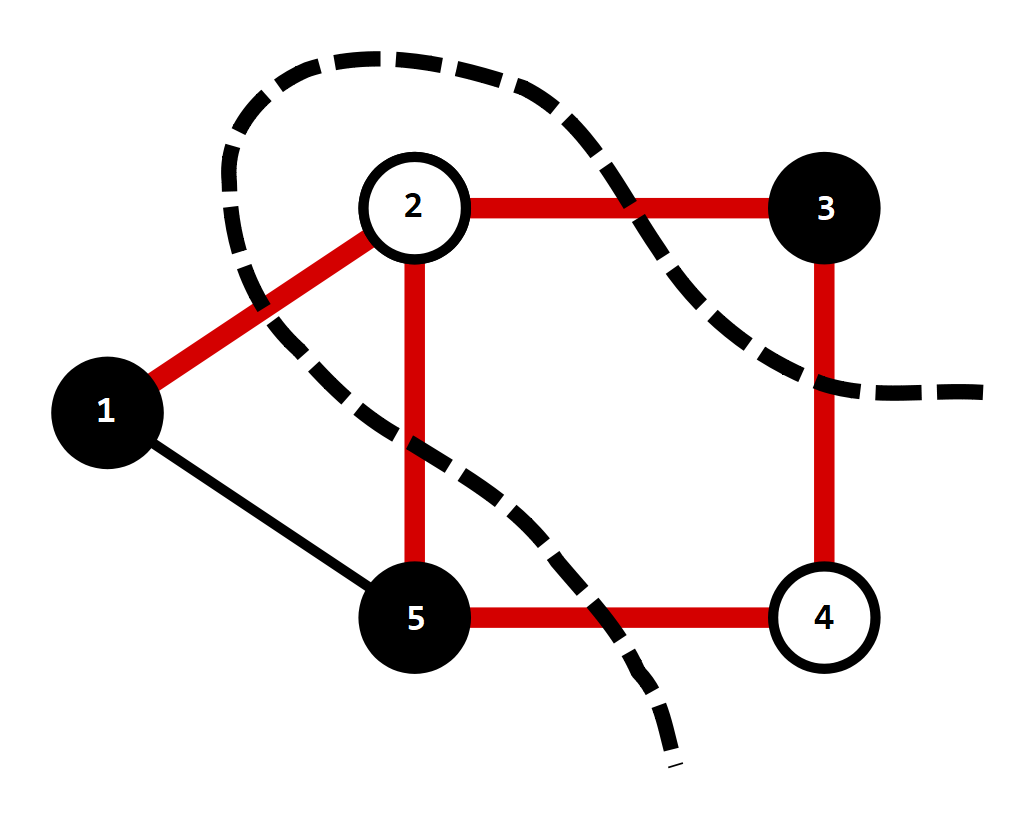
\includegraphics[width=0.5\textwidth]{figures/MaxCut.png}
	\caption{An example of the Max-Cut problem on a graph with 5 nodes. The nodes are partitioned into two sets; black nodes and white nodes. The goal is to maximize the number of edges between the two sets (these are colored red). More generally when talking about weighted graphs we want to maximize the sum of the weights of the edges connecting the two sets. Figure from \cite{wiki:MaxCut}}
	\label{fig:MaxCut}
\end{figure}

For reasons that will become apparent in Chapter \ref{chap:qaoa}, it is sometimes useful to write the bipartition in terms of a bit string. A bit string is simply a sequence of bits, usually denoted by $0$ or $1$. This can be achieved by labelling the $n$ vertices in a particular order $(1, \dots, n)$. By using the fact that the partition is completely characterized by \emph{one} set $S$, we can represent a partition of $V$ into $S$ and $\bar{S}$ by a bit string $\vec{x}$ consisting of ones and zeros. We can translate between the two using the function $f: \mathcal{P}(V) \mapsto \{0,1\}^{n}$ defined by
\begin{equation}
	f(S) = \big(\mathbf{1}_S(1), \dots, \mathbf{1}_S(n) \big)
\end{equation}
where $\mathcal{P}(V)$ denotes the powerset of $V$, and $\mathbf{1}_{S}$ denotes the characteristic function of $S$. For example, let us label the vertices in Figure \ref{fig:MaxCut} in clockwise fashion starting from the leftmost vertex. We can represent the cut shown as $\vec{x} = (1,0,1,0,1)$, where the black nodes constitute set $S$ and the white nodes consitute set $\bar{S}$. The objective function in terms of $\vec{x}\in \{0,1\}^n$ becomes
\begin{equation}
C(\vec{x}) = \sum_{\{i,j\} \in E} w_{i,j}(x_i-x_j)^2
\label{eq:maxcut bitstring objective}
\end{equation}
Equivalently, we can use a binary string $\vec{z} \in \{-1,1\}^n$. The objective function is then described by
\begin{equation}
	C(\vec{z}) = \sum_{\{i,j\} \in E}\frac{w_{i,j}}{2}(1-z_iz_j)
\end{equation}
This approach will become useful in the next chapter, where we will talk about spins.

\newpage
\section{Approximation algorithms and ratios}
% NP complete
The Max-Cut problem is an example of a problem that is NP-complete \cite{Karp72}. NP-completeness implies NP-hardness which roughly means we have to resort to extensive searching in order to find the optimal cut. To be more precise, no polynomial-time algorithms for Max-Cut are known for arbitrary graphs. Therefore, we have to resort to finding good solutions instead. One approach to find such good solutions is to design approximation algorithms. These algorithms seek to find solutions that guarantee the objective value to be at least the optimum times a certain ratio, called the approximation ratio $\rho$.
\begin{equation}
\frac{C(\vec{x})}{C_{\max}} \geq \rho
\end{equation}
where $C_{\max} = \max_{\vec{x}} C(\vec{x})$. Note that $\rho \leq 1$ as we can not do better than the optimal solution. Note that these algorithms grant a guarantee that the objective value for a found solution $\vec{x}$ lies in a particular range
\begin{equation}
\rho C_{\max} \leq C(\vec{x}) \leq C_{\max} 
\end{equation}
It certainly might be the case that for particular instances of the problem an approximation algorithm finds solutions that are better than $\rho C_{\max}$.

\subsection{Bounds on the approximation ratio of Max-Cut}
In 2002 the Swedish theoretical computer scientist H\r{a}stad proved that it is NP-hard to approximate the Max-Cut value with an approximation ratio better than $\frac{16}{17} \approx 0.941$  for Max-Cut on all graphs \cite{Hastad02}, or $331/333 \approx 0.994$ when restricted to unweighted 3-regular graphs \cite{BK99}. As the approximation ratio for polynomial-time algorithms for Max-Cut is bounded, this means that the problem is in the class APX, for approximable problems.

In addition, there is a conjecture from theoretical computer science called the Unique Games Conjecture (UGC) \cite{UGC}. The conjecture postulates that the problem of determining the approximate value of a unique game, is NP-hard. The details of the Unique Games Conjecture are rather technical and not relevant for the rest of this work, I refer the interested reader to the original paper \cite{UGC}, or to \cite{UGC-Blog} for a less formal discussion. However, there is a consequence of the conjecture that is relevant. It turns out that if the UGC is true, then there exists no polynomial time algorithm that can beat Goemans-Williamson \cite{KKMO05}, thus restricting the possible approximation ratio even further to around $0.878$. 

At the moment, it is unknown whether or not the conjecture is true, but it is interesting to note that an approximation algorithm that is better than Goemans-Williamson would imply that the UGC is false. Unlike the question whether or not $P = NP$, currently there seems to be no consensus in the academic world around the Unique Games Conjecture.

\section{Classical Algorithms for Max-Cut}
In this section I will discuss known classical algorithms for solving Max-Cut to give a sense of what is already possible on classical computers. The presentation of the algorithms in the coming subsections largely follows the structure of \cite{lecture-MaxCut, lecture-GW}.
\subsection{Greedy approach}
One algorithm for solving Max-Cut uses a greedy approach and guarantees an approximation ratio of $\frac{1}{2}$. 

Let $G(V,E)$ be an undirected graph with edge weights $w_e$ for $e\in E$ and label $V = \{1, \dots n\}$ so there is some ordering. Next, define $E_i = \{(k,i) : \{k,i\} \in E, k < i\}$, the set of edges entering vertex $i$ from ``lower'' nodes. Note that $E_i \cap E_j = \emptyset$ if $i \neq j$ because of the strict inequality. Initially, set $S = \{1\}$ and $\bar{S} = \emptyset$.  Then starting from $i=2$, add node $i$ to either $S$ or $\bar{S}$ so that the sum of the number of edges in $E_i$ that are in the cut times their respective weights is maximized. Increment $i$ and repeat the last step until $i=n$.

As an example, consider the graph from Figure \ref{fig:MaxCut}. For simplicity I will consider it to be an unweighted graph with $w_{i,j} = 1$ for all $\{i,j\}\in E$. Starting with $S = \{1\}$, consider node $2$. We choose to add node $2$ based on what choice maximizes $\sum_{e \in E_2 \cap K(S)}w_e$, which in our case is simple: we add node $2$ to set $\bar{S}$ because then edge $(1,2)$ is in the cut. We move on to node $3$ with $E_3 = \{(2,3)\}$, and we choose node $3$ to be in $S$ because then edge $(2,3)$ is in the cut. Analogously, we add edge $4$ to $\bar{S}$. Node $5$ is somewhat more tricky as we have $E_5 = \{(1,5),(2,5),(4,5)\}$ containing 3 edges instead of just one. Adding node $5$ to $S$ would yield $\sum_{e \in E_5 \cap K(S)}w_e = 2$ while adding it to $\bar{S}$ would yield $\sum_{e \in E_5 \cap K(S)}w_e = 1$. Therefore, we add node $5$ to $S$ and we are done. The final result is thus $S = \{1,3,5\}$ and $\bar{S} = \{2,4\}$ with a cutvalue of 5, which is actually optimal.
\\

Let us proof that this is indeed an approximation algorithm with approximation ratio $\frac{1}{2}$. Define $K$ to be the cut obtained by the algorithm, and observe that $E_1, \dots E_n$ is a partition of $E$ as the sets are pairwise disjoint and $E = \bigcup_i E_i$. For each node $i \in V$, define $\tilde{E}_i = E_i \cap K$. Note that the cut $K$ is the union of these newly constructed sets $K = \bigcup_i \tilde{E}_i$. The finalizing observation is that we chose $S,\bar{S}$ in such a way that 
\begin{equation}
\sum_{e\in \tilde{E}_i}w_e \geq \frac{1}{2}\sum_{e \in E_i}w_e \qquad \forall i \in V
\end{equation}
Therefore we have that 
\begin{equation}
	C(S) = \sum_{i\in V} \sum_{e \in \tilde{E}_i} w_e \geq \frac{1}{2}\sum_{i\in V} \sum_{e \in E_i} w_e = \frac{1}{2}\sum_{e\in E} w_e \geq \frac{1}{2}C_{\max}
\end{equation}
where the latter inequality is derived from the fact that the optimum cut can not be larger than the sum of the weights of all edges.

\subsection{Random partition}
\label{sec:random-partition}
Another algorithm for solving Max-Cut that is quite easy to implement is simply choosing a random partition. As the name suggests, it is a stochastic algorithm. 

Let $G = (V,E)$ again be an undirected graph. We choose each vertex in $V$ to be in either $S$ or $\bar{S}$ with equal probability $\frac{1}{2}$. This bipartition defines a cut $K(S)$, whose expected size we will now calculate. 

Consider an edge $e \in E$ in the graph. Remark that $\prob{e \in K(S)} = \frac{1}{2}$. For $e \in E$, we define $\chi_e$ to be a random variable such that $\chi_e = 1$ if $e \in K(S)$ and $\chi_e = 0$ if $e \notin K(S)$. The value of the cut is then
\begin{equation}
	C(S) = \sum_{e\in E} w_e\chi_e
\end{equation}
Note that the value itself is now a random variable, so we have to resort to calculating the expecation value of the cut. Using linearity of the expectation operator, we obtain the following
\begin{equation}
	\expect{C(S)} = \sum_{e \in E} w_e\expect{\chi_e} = \sum_{e \in E}w_e \prob{e \in K(S)} = \frac{1}{2}\sum_{e \in E}w_e \geq \frac{1}{2}C_{\max}
\end{equation}
Resulting in a $\frac{1}{2}$-approximation ratio in expectation. I would like to emphasize that we give a lower bound for the expectation value of the objective function, and not a lower bound for every outcome. Note that it might be the case that the algorithm produces with probability $2^{-n}$ a partition $S = V, \bar{S} = \emptyset$ with a cutvalue of 0. 

\subsection{Goemans-Williamson}
The best classical approximation algorithm for solving Max-Cut known is the algorithm proposed by Goemans and Williamson (GW) in 1994 \cite{GW95}. The algorithm is also stochastic and has an approximation ratio $\rho \approx 0.878$ in expectation. Prior to GW, the best-known approximation algorithms for the Max-Cut problem had performance guarantee of $\frac{1}{2} + o(1)$, meaning that the achieved approximation ratio is below $\frac{1}{2} + \epsilon$ for any $\epsilon>0$. The GW-algorithm was indeed quite a breakthrough. 

The algorithm uses a sophisticated method that randomly rounds the solution to a nonlinear programming relaxation. Before I will present the algorithm, the following two definitions are useful.

\begin{definition}
	A square $n \times n$ matrix $A$ is called \textbf{positive semidefinite} if the following holds
	\begin{equation}
	\vec{x}^TA \vec{x} \geq 0 \qquad \forall \vec{x} \in \mathbb{R}^n
	\end{equation} 
	This property is sometimes indicated using $A \succcurlyeq 0$
\end{definition} 

\begin{definition}
	 A \textbf{semidefinite program} is the problem of optimizing a
	linear function of a symmetric positive semidefinite matrix subject to linear equality constraints.
\end{definition}
Indeed a semidefinite program is a subclass of the more general linear programs, so it is possible to solve these using the well known Simplex method \cite{simplex}. While the Simplex method itself is not a polynomial time algorithm, it can be generalized to semidefinite programs \cite{pataki}. Given any $\epsilon >0$ these semidefinite programs can be solved in polynomial time within an additive error of $\epsilon$. This can be done using a variety of methods, these include interior point methods \cite{nesterov1994interior}, the ellipsoid method \cite{lovasz1988geometric}, and other polynomial-time algorithms for convex programming \cite{vaidya}.

The problem to be solved is

\begin{maxi!}|l|
	{\vec{z}}{\frac{1}{4}\sum_{\{i,j\}\in E}w_{i,j}(z_i-z_j)^2}
	{}{}
	\label{probleem1}
	\addConstraint{z_i \in \{-1,1\} \text{ for } i \in V}
	\label{probleem2}
\end{maxi!}
which is equivalent to what we saw in \eqref{eq:maxcut bitstring objective}.
Let us denote the optimal solution of this program as $C_{\max}$. Next, we introduce a \emph{relaxation} of the problem meaning that we let loose of some of the constraints in order to make solving it easier
\begin{maxi!}|l|
	{\vec{z}}{\frac{1}{4}\sum_{\{i,j\}\in E}w_{i,j}(\vec{y}_i\cdot \vec{y}_i + \vec{y}_j\cdot \vec{y}_j - 2\vec{y}_i\cdot \vec{y}_j)}
	{}{}
	\addConstraint{\vec{y}_i \in \mathbb{R}^n \text{ and } \|\vec{y}_i\|^2 = 1 \text{ for } i \in V}
\end{maxi!}
Note that the above problem is indeed a relaxation, as we can simply take $\vec{y}_i = z_i \vec{e}_1$ to reconstruct program \eqref{probleem1}, \eqref{probleem2}, where $\vec{e}_1$ is the first standard basis vector of $\mathbb{R}^n$. Let me denote the optimal solution of the relaxation as $\tilde{C}_{\max}$, then we have $\tilde{C}_{\max} \geq C_{\max}$. The above so called vector program is equivalent to the following semidefinite program, where we define a matrix $A = (a_{ij})$
\begin{maxi!}|l|
	{\vec{z}}{\frac{1}{4}\sum_{\{i,j\}\in E}w_{i,j}(a_{ii}+a_{jj}-2a_{ij})}
	{}{}
	\addConstraint{a_{ii} = 1 \text{ for } i \in V \text{ and } A \succcurlyeq 0} \text{ and symmetric}
\end{maxi!}

This semidefinite program can be solved in polynomial time obtaining an optimal matrix $A^*$ with value $c$. Note that the solution could be irrational. In that case we can find an approximation that is rational in polynomial time with value $c'$ with $c - \epsilon < c' < c$ for any $\epsilon > 0$. Using the symmetry of the semidefinite matrix $A^*$ we know that we can decompose $A^* = U^TU$ where $U$ is an $m \times n$  matrix with $m \leq n$, this is called the Cholesky decomposition. Next, we consider the column vectors of $U = \{\vec{u}_1,\dots \vec{u}_n\}$. Because of the semideniteness of $A^*$ and the constraint that $a_{ii}^* =1$, we know that these are unit vectors $\|\vec{u}_i\|^2 = \vec{u}_i^T\vec{u}_i = a^*_{ii} = 1$. Moreover, we know that $\vec{u}_i \in \mathbb{R}^m$ for $i = 1, \dots, n$ and since $m \leq n$ we can embed these vectors in $\mathbb{R}^n$. Thereafter, we randomly choose a hyperplane through the origin, and in polynomial time we can figure out which vectors are above or below the hyperplane. The vectors $\vec{u}_i$ that lay above the plane denote vertices that are on one side of the partition, and the vectors $\vec{u}_i$ below the plane denote the vertices that are on the other side of the partition.

Using a combination of geometric arguments and insights from calculus, it can be shown that the algorithm has an approximation ratio of 
\begin{equation}
\rho = \frac{2}{\pi} \min_{0 \leq \theta \leq \pi} \frac{\theta}{1 - \cos \theta}
\end{equation}
in expectation, which numerically evaluates to $\rho \approx 0.878$ \cite{GW95}. 

For a more extensive discussion of the Goemans-Williamson algorithm I refer to \cite{GW95,GW-lecture-Hollbach,lecture-GW}.

\section{Applications of Max-Cut}
The maximum cut problem is a natural and simple to understand graph problem often discussed in introductory optimization or algorithm courses. There are also some applications of the problem. An example of which is efficient design of electric circuits or communication networks \cite{wang2010maximum}, but the problem also has uses in statistical physics, namely in finding the groundstate energy in spin glass \cite{maxcut-applications}.

\subsection{Ising Model} %maybe a paragraph is more suitable
The Ising model describes a system of $n$ particles with two possible states, for example spin up and down. See Figure \ref{fig:ising-model} for an illustration. The system can then be characterized by a binary string $\sigma \in \{-1,1\}^n$. Following the example, $1$ denotes spin up and $-1$ denotes spin down. The Hamiltonian reads as follows
\begin{equation}
H(\sigma) = \sum_{\{i,j\}} J_{ij} \sigma_i \sigma_j - \mu \sum_i h_i \sigma_i 
\end{equation}
where the first sum is over the adjacent pairs $\{i,j\}$ in the system, and $J_{ij}$ designates the strength of the interaction of the constituents of that pair. The second sum describes the interaction with some magnetic field, with strength $h_i$ at site $i$. Note that when there is no external magnetic field, i.e. $h_i = 0$ for all $i$, then the problem of finding a groundstate is equivalent to the Max-Cut problem. Closely related to the Ising model is the Sherrington-Kirkpatrick model. 

\begin{figure}[H]
	\centering
	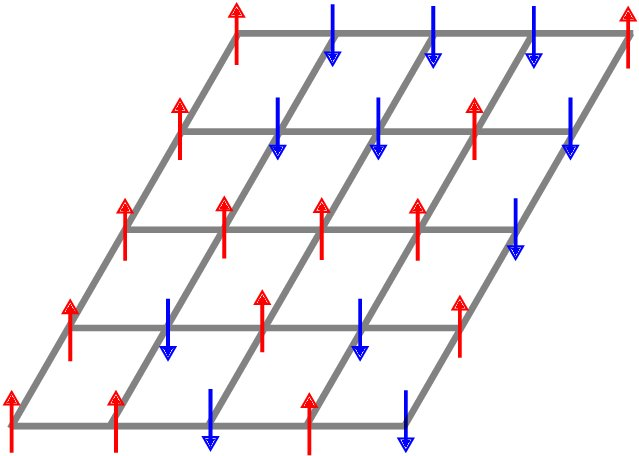
\includegraphics[width=0.5\textwidth]{figures/Ising-model-on-a-square-lattice.jpg}
	\caption{Schematic representation of a configuration of the 2D Ising model on a square lattice. Figure and caption from \cite{ising-model}}
	\label{fig:ising-model}
\end{figure}
\chapter{The Quantum Approximate Optimization Algorithm}
\label{chap:qaoa}

The Quantum Approximate Optimization Algorithm, abbreviated QAOA, was proposed by Farhi, Goldstone and Gutmann in 2014 \cite{FGG14}. The goal of the algorithm is finding approximate solutions to combinatorial optimization problems. Due to its shallow depth it is feasible to run it without error correction on NISQ devides, making it interesting for near-term implementation. The quantum circuit that implements the algorithm prepares a parametrized state, and consists of $p$ layers. Each of the layers comprises of two unitary operators, the first encoding the problem and the latter entangling the qubits, parametrized by some angles. Appropriate parameters can be found in a variety of ways, the most popular being a variational approach similar to the variational quantum eigensolver \cite{VQE}. By sampling from this parametrized state an approximate solution to the problem can be found.
\\

There are two main reasons why QAOA is promising for solving combinatorial optimization problems. First of all because it can be shown that adding extra layers monotonically improves the result of the algorithm. Additionally, in the limit $p \to \infty$, the algorithm produces the optimum, similar to the quantum adiabatic algorithm \cite{FGG14}. Secondly, it is interesting because of its potential to exhibit quantum supremacy \cite{FH16}, as it can not be efficiently simulated by a classical computer. Because of this potential, the algorithm has received quite some attention from the scientific community in the last few years and continues to do so.
\\

In this chapter, I will give an overview of prior work that has been done on QAOA. Specifically, I will explain the general algorithm, how the algorithm can be applied to Max-Cut and how it relates to the Quantum Adiabatic Algorithm that was proposed in \cite{FGGS2000} in 2000. 

\section{General setup}
\label{sec:general-setup}
The Quantum Approximate Optimization Algorithm is designed to handle general optimization problems. These problems can be specified by $n$ bits and $m$ clauses, where a clause is a constraint on a subset of the bits which is satisfied for certain assignments of those bits and not satisfied for other assignments. We want to find a bit string $\vec{x} \in \{0,1\}^n$ of size $n$ that maximizes or minimizes a cost function \cite{FGG14}
\begin{equation}
	C(\vec{x}) \define \sum_{\alpha=1}^m C_\alpha(\vec{x})
	\label{eq:objective}
\end{equation}
where we sum over $m$ clauses that depend on a subset of the $n$ bits. We define $C_\alpha = 1$ if clause $\alpha$ is satisfied and $C_\alpha=0$ otherwise. The goal is to satisfy as many clauses as possible, as that we want to maximize $C(\vec{x})$.
\\
The QAOA is a quantum algorithm that is aimed to find a bit string $\vec{x}'$ for which $C(\vec{x}')$ is close to the maximum of $C$. A quantum computer works in a $2^n$ dimensional vector space, more precisely a Hilbert space in which the norm is induced by an inner product. The computational basis vectors $|\vec{x}\rangle$ can be represented by bit string consisting of $0$s and $1$s. We can consider both the objective function $C$ and the clause $C_\alpha$ in \eqref{eq:objective} as operators that are diagonal in the computational basis.
\begin{equation}
	\hat{C} = \sum_{\vec{x}\in\{0,1\}^n} C(\vec{x})\cdot |\vec{x}\rangle\langle \vec{x} | =  \sum_{\alpha=1}^m \hat{C}_\alpha
	\qquad \text{where} \qquad 
	\hat{C}_\alpha = \sum_{\vec{x}\in\{0,1\}^n} C_\alpha(\vec{x})\cdot |\vec{x}\rangle\langle \vec{x} | = \begin{bmatrix}
	C_\alpha(0, \dots, 0) &  & \\
	& \ddots & \\
	& & C_\alpha(1,\dots, 1)
	\end{bmatrix}
	\label{eq:costHamiltonian}
\end{equation}
We call $\hat{C}$ the \textbf{cost Hamiltonian}. To avoid confusion, I will refer to the operators above as $H_C \equiv \hat{C}$ and $H_{C_\alpha} \equiv \hat{C}_\alpha$ for the rest of this thesis, following the notation from \cite{Hidary}. Using the operator $H_C$, we define the operator $U(H_C, \gamma)$ which depends on some real valued angle $\gamma \in \mathbb{R}$ as follows

\begin{equation}
	U(H_C,\gamma) \define e^{-i\gamma H_C } = \prod_{\alpha = 1}^m e^{-i\gamma H_{C_\alpha}}
	\label{eq:costUnitary}
\end{equation}
I will refer to this object as the \textbf{cost unitary}. Note that the cost Hamiltonian from \eqref{eq:costHamiltonian} is Hermitian, and therefore has purely real eigenvalues, hence the operator $U(H_C,\gamma)$ is indeed unitary. Moreover, observe that the latter equality from \eqref{eq:costUnitary} comes with a caveat. As we want to be able to write $U(H_C, \gamma)$ as a product of local terms it is important that the $H_{C_\alpha}$ commute pairwise. 

\begin{remark}
Remember that the definition of the matrix exponential is derived from the Taylor expansion of the exponent. The exponential of matrix $A$ is given by
\begin{equation}
e^A = \sum_{k=0}^{\infty} \frac{1}{k!}A^k = I + A + \frac{1}{2}A^2 + \frac{1}{6}A^3 + \dots
\end{equation}
Different than taking the exponential of real numbers, the following equality does not always hold for matrix exponents because of possible noncommutativity.
\begin{equation}
e^{A+B} \myeq{?} e^A e^B
\label{eq:matrix-exponential}
\end{equation}
Observe that
\begin{equation}
	e^{A+B} = I + (A+B) + \frac{1}{2}(A+B)^2 + \dots = I + A+B + \frac{1}{2}(A^2 + AB + BA + B^2) + \dots
\end{equation}
\begin{equation}
	e^{A}e^{B} = (I + A + \frac{1}{2}A^2 + \dots)(I + B + \frac{1}{2}B^2 + \dots) = I + A + B + \frac{1}{2}(A^2+2AB+B^2) + \dots
\end{equation}
It can be shown that \eqref{eq:matrix-exponential} only holds if $A$ and $B$ commute, this statement can be extended for arbitrary finite sums. Hence, it is essential for $H_{C_\alpha}$ to commute when separating the cost unitary into local terms in \eqref{eq:costUnitary}.
\end{remark}
If we give every clause equal weight $w_\alpha = 1$, we know that the cost Hamiltonian is diagonal with solely integer entries, which are precisely the eigenvalues of the matrix. We can use the fact that $H_C$ has integer eigenvalues in order to restrict $\gamma$ to be in $[0,2\pi)$. The approach of translating an objective function to an operator is very general and can be applied to a variety of problems. The actual form of $H_C$ is be determined by the specific problem. In section \ref{sec:maxcut-qaoa} I will discuss it in the case of Max-Cut.

Next, we define the operator $H_B$, called the \textbf{mixer Hamiltonian}
\begin{equation}
	H_B \define \sum_{j=1}^n \sigma_x^{(j)}
	\label{eq:mixerHam}
\end{equation}
where $\sigma_x^{(j)}$ is the Pauli-$X$ gate acting solely on the qubit $j$.
\begin{equation}
	\sigma_x^{(j)} = I^{\otimes j-1} \otimes \sigma_x \otimes I^{\otimes n-j}
\end{equation}
where $I$ is the $2\times 2$ identity matrix, $\otimes$ denotes the Kronecker product and $A^{\otimes n}$ denotes the Kronecker product of a matrix $A$ with itself $n$ times. 
\begin{equation}
	A^{\otimes n} = \underbrace{A \otimes \dots \otimes A}_{n \text{ times}}
\end{equation}

Using the mixer Hamiltonian, we can define another unitary operator, the \textbf{mixer unitary}, similar to what we did before
\begin{equation}
	U(H_B,\beta) \define e^{-i\beta H_B} = \prod_{j=1}^n e^{-i \beta \sigma_x^{(j)}}
	\label{eq:mixerUnitary}
\end{equation}

where again $\beta \in \mathbb{R}$ is some real angle. Note that $\sigma_x^{(j)}$ commute pairwise so when taking the exponential of $H_B$ that is the sum of these terms, expression \eqref{eq:matrix-exponential} holds and we are able to construct $H_B$ with local gates. With these unitaries defined, we can move on to the next part: preparing the parameterized state. We start of in the initial equal superposition state
\begin{equation}
	|s\rangle \define \frac{1}{\sqrt{2^n}}\sum_{x\in \{0,1\}^n} |x \rangle = |+\rangle^{\otimes n} = H^{\otimes n}|0\rangle^{\otimes n}
\end{equation} 
which is easy to prepare using Hadamard gates applied to each of the $n$ qubits, all in the state $|0\rangle$. 
Thereafter, we alternately apply the cost Hamiltonian and the mixer Hamiltonian $p$ times, using different parameters $\gamma_1 \dots \gamma_p$ and $\beta_1 \dots \beta_p$, respectively. 
\begin{equation}
	|\vec{\gamma}, \vec{\beta}\rangle \define \underbrace{ U(H_B,\beta_p)U(H_C,\gamma_p) \dots \underbrace{U(H_B,\beta_1)U(H_C,\gamma_1)}_{\text{one layer}}}_{p \text{ layers}}|s\rangle
\end{equation}
I use boldface vector notation $\gambe$ for the sole purpose of writing these sets of parameters more compactly. Furthermore, take note that we work from right to left, as is convention when working with matrices. See Figure \ref{fig:schematic-qaoa} for a schematic of the circuit preparing the parametrized state. Now that we have established this, we can move on to the actual aim of this circuit. The idea is to find parameters such that 
\begin{equation}
	F_p(\gambe) \define \langle \gambe |H_C| \gambe \rangle
\end{equation}
is maximized, where we indicate the number of layers $p$ using a subscript. In general, $\vec{\gamma},\vec{\beta} \in \mathbb{R}^p$, however depending on the cost and mixer unitaries we can restrict the domain using symmetries. We define 
\begin{equation}
M_p \define \max_{\gambe} F_p(\gambe)
\end{equation} and want to find the corresponding parameters. By sampling from this state $|\gambe \rangle$ we can find an approximate solution by looking at either the most sampled bit string, or the best sampled bit string.

The reader might wonder why we need to apply the mixer unitary when only the cost unitary encodes the problem. This has to do with the way probabilities work in quantum mechanics. The probability of measuring a bit string that encodes a particular solution, is precisely the square magnitude of the corresponding amplitude. Take note of the fact that the exponent of a diagonal $n \times n$ matrix $A = \diag{a_{11}, \dots a_{nn}}$ is a diagonal matrix with the entries exponentiated.  
\begin{equation}
	e^{\diag{a_{11},\dots a_{nn}}} = \diag{e^{a_{11}},\dots, e^{a_{nn}}}
\end{equation}

Since the cost Hamiltonian $H_C$ is diagonal and real, the cost unitary will be diagonal with entries of the form $e^{i\phi}$ for some $\phi \in \mathbb{R}$. This implies that the amplitudes will only acquire relative phases, and thus the probability of finding a particular bit string is not affected by the cost unitary. If we were going to run a circuit with only cost unitaries, it would result in an equal superposition, whatever set of angles $\vec{\gamma}$ we choose. A fancy way of implementing the random partition algorithm from Section \ref{sec:random-partition}. For this reason we need an operator that entangles the states to do better than the random partition algorithm, hence the need for the mixer Hamiltonian.

Finding the optimal, or even a good set of angles $\gambe$ is a non-trivial task. In Section \ref{sec:optimal-parameters} a more thorough discussion on this topic can be found. Furthermore, one method for finding the angles proposed in \cite{ZWCPL18}, called INTERP, is discussed in more depth in Chapter \ref{chap:implementation}, which will also be used to produce the results in Chapter \ref{chap:results}.

\begin{figure}[H]
	\centering
	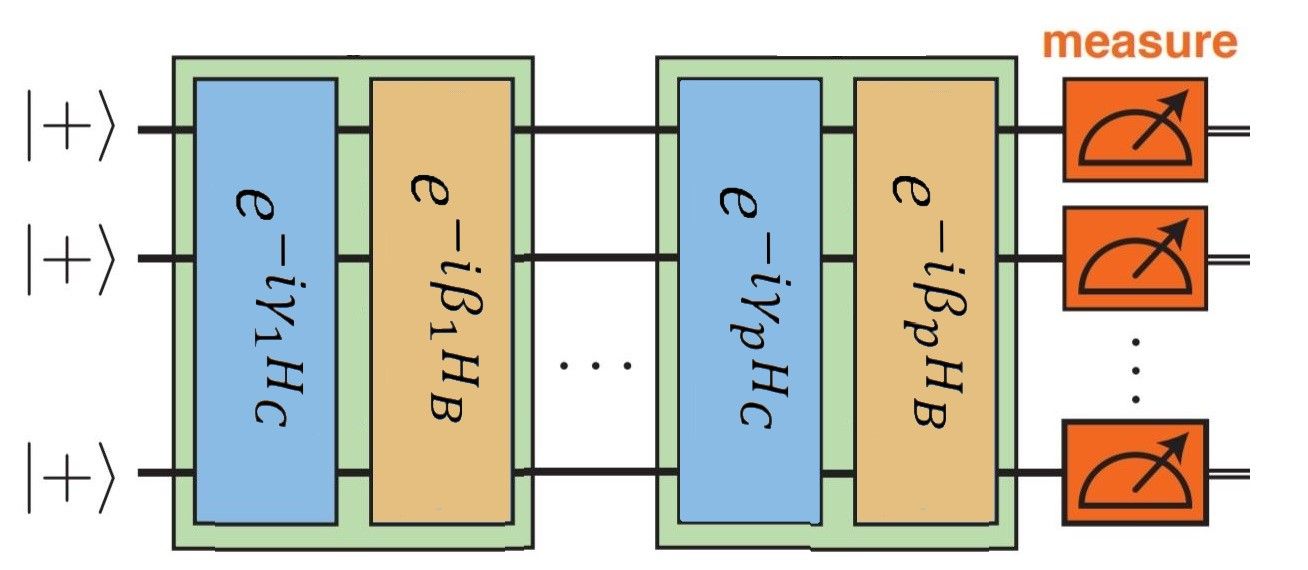
\includegraphics[width=0.8\textwidth]{figures/qaoa_idea_edit.JPG}
	\caption{Schematic of a $p$-level Quantum Approximation Optimization Algorithm. The cost unitary and the mixer unitary are alternately applied to prepare the parametrized state $|\gambe\rangle$. Adapted figure from \cite{ZWCPL18}.}
	\label{fig:schematic-qaoa}
\end{figure}

\section{Applying QAOA to Max-Cut}
\label{sec:maxcut-qaoa}
QAOA can easily be applied to the Max-Cut problem by associating each vertex $i \in V$ with a qubit $q_i$ and using the qubit's state to encode the affiliation to one of the sets of the bipartition. A qubit in state $|1\rangle$ means it is in one half of the bipartition, $S$, a qubit in state $|0\rangle$ means it is in the other, namely $\bar{S}$. Our aim is to find a cut such that we maximize the sum of the edges in the cut, so we would like adjacent qubits to be in different halves of the bipartition. As explained in Section \ref{section:maxcut}, we can express this mathematically as
\begin{equation}
	C(\vec{z}) = \frac{1}{2}\sum_{\{i,j\}\in E} w_{i,j}(1-z_i z_j)
\end{equation}
where $z_i \in \{-1,1\}$ for $i\in V$. Now the idea is to translate this problem into a cost Hamiltonian. Remark that the Pauli matrix $\sigma_z = \diag{1,-1}$ has eigenvalues $1$ and $-1$. Therefore, we can use $\sigma_z^{(i)}$ to represent $z_i$. Using this we can define the cost Hamiltonian to be
\begin{equation}
	H_C = \frac{1}{2} \sum_{\{i,j\}\in E} w_{i,j}\big(I-\sigma_z^{(i)}\sigma_z^{(j)}\big)
\end{equation}
Note that the term $I-\sigma_z^{(i)}\sigma_z^{(j)}$ involving qubits $i$ and $j$ is diagonal in the computational basis. This is important because we want to be able to write the cost unitary as a product of local terms
\begin{equation}
	U(H_C, \gamma) = e^{-i\gamma H_C} = \prod_{\alpha=1}^m e^{-\gamma H_{C_\alpha}} = \prod_{\{i,j\}\in E} e^{-\gamma \frac{w_{i,j}}{2}\big(I-\sigma_z^{i}\sigma_z^{j}\big)}
\end{equation}
Since all the terms in the product are diagonal, they all commute as desired. Now we have all the ingredients to prepare the state $|\gambe\rangle$ for Max-Cut using the unitary operators $U(H_C, \gamma)$ and $U(H_B, \beta)$. 

The actual outcome of the algorithm is determined by sampling from the state $|\gambe\rangle$ and calculating the cut value corresponding to the measured bit string on a classical computer. This yields a distribution of bit strings (and cutvalues). However, in the end we want one solution and not a distribution. One option would be to pick the most sampled bit string, but performance is easily improved by picking the best sampled bit string instead.

Now, we only need to find out how to implement this in a circuit and figure out a way for finding appropriate angles $\gambe$. This will be discussed in Subsection \ref{subsec:circuit} and Section \ref{sec:optimal-parameters}, respectively.

\subsection{Quantum circuit design}
\label{subsec:circuit}
It is useful to know about the rotation operators $R_x$ and $R_z$ when wanting to implement the unitary operators $U(H_C,\gamma), U(H_B,\beta)$. These operators induce rotations around their respective axes, and are defined as follows
\begin{equation}
		R_x(\theta) \equiv e^{-\frac{\theta i}{2} \sigma_x} = \begin{bmatrix}
			\cos(\theta/2) & -i\sin(\theta/2) \\
			-i\sin(\theta/2) & \cos(\theta/2)
		\end{bmatrix}
\end{equation}
\begin{equation}
	R_z(\theta) \equiv e^{-i\frac{\theta}{2} \sigma_z} = \begin{bmatrix}
	e^{-i \theta /2} & 0 \\
		0 & e^{i\theta/2}
	\end{bmatrix}
\end{equation}
Furthermore, we need a $\CNOT$ gate \cite{Mike&Ike}, which involves 2 qubits
\begin{equation}
	\CNOT_{q_i,q_j} = |0\rangle \langle0| \otimes I + |1\rangle \langle1|\otimes X  = \begin{bmatrix}
	1 & 0 & 0 & 0 \\
	0 & 1 & 0 & 0 \\
	0 & 0 & 0 & 1 \\
	0 & 0 & 1 & 0 \\
	\end{bmatrix} 
	= 
	\Qcircuit @C=1em @R=.7em {
		&q_i& & \ctrl{1} & \qw  \\
		&q_j& & \targ  & \qw \\
	}
\end{equation}
To understand this component intuitively, the target qubit $q_j$ will be flipped if the control qubit $q_i$ is $1$. As we are working with qubits, this does not encapsulate the complete picture, so we need to describe it with a matrix instead. 

The $X$-interactions in the mixer Hamiltonian can be implemented with this one-qubit gate $R_x$.
\begin{equation}
	e^{-i\beta\sigma_x^{(i)}} \equiv \Qcircuit @C=1em @R=.7em {
		&q_i& & \gate{R_x(2\beta)}  & \qw\\
	}
\end{equation}
The two-qubit $ZZ$-interactions in the cost unitary can be implemented with two $\CNOT$ gates, and the local one-qubit gate $R_z$ \cite{Crooks18}. Since $\sigma_z^{(i)}$ and $\sigma_z^{(j)}$ commute the roles of $q_i$ and $q_j$ are interchangable.
\begin{equation}
e^{-\frac{i}{2}\gamma(I-\sigma_z^{(i)}\sigma_z^{(j)})} \equiv \Qcircuit @C=1em @R=.7em {
	&q_i& & \ctrl{1} & \qw & \ctrl{1}  & \qw \\
	&q_j& & \targ \qw & \gate{R_z(-\gamma)} & \targ & \qw\\
} 
\equiv 
\Qcircuit @C=1em @R=.7em {
	&q_i& & \targ \qw & \gate{R_z(-\gamma)} & \targ & \qw\\
	&q_j& & \ctrl{-1} & \qw & \ctrl{-1}  & \qw \\
} 
\end{equation}

As both $U(H_C,\gamma)$ and $U(H_B,\beta)$ are both products of local terms, we only need those terms to implement them. The final circuit first applies Hadamards to each qubit in order to create an equal superposition over all bit strings, or possible partitions if you will. Next we apply the cost unitary and the mixer unitary in an alternating fashion, in that order, with desired angles. Lastly, we measure the state to get an actual bit string.

As an example, consider the unweighted \emph{diamond graph}, visualised in Figure \ref{fig:graph-diamond}. 

\begin{figure}[H]
	\centering
	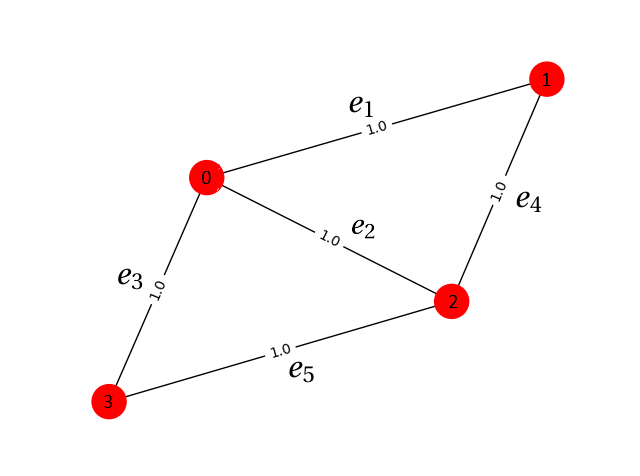
\includegraphics[width=0.35\textwidth]{figures/diamond-graph-edges}
	\caption{Diamond graph (unweighted)}
	\label{fig:graph-diamond}
\end{figure}

The graph consists of 4 nodes, whereof 2 nodes connect to 2 edges, and 2 nodes connect to 3 edges. The circuit needed to prepare the state $|\gamma,\beta \rangle$ with $p=1$ for this particular graph is given in Figure \ref{fig:circuit}.
In general, the depth of the circuit, assuming no overhead necessary for swapping is then at most $p(3m+n)$ where $p$ is the number of QAOA layers, $n$ is the number of nodes, or qubits and $m$ is the number of edges in the graph. For a graph with $n$ nodes we can bound $m$ by $\frac{1}{2}n(n-1)$, the number of edges in a complete graph. Concluding, we see that the circuit requires $O(n^2)$ gates assuming full qubit connectivity. %In actual hardware one usually encounters qubits arranged in a 2-dimensional lattice with gates only between nearest neighbours. Hence, SWAP gates are necessary to move logical qubits into proximity. It turns out that QAOA can be efficiently implemented with $O(n)$ overhead \cite{Crooks18}.  \hl{elab on swaps}

\begin{figure}[H]
	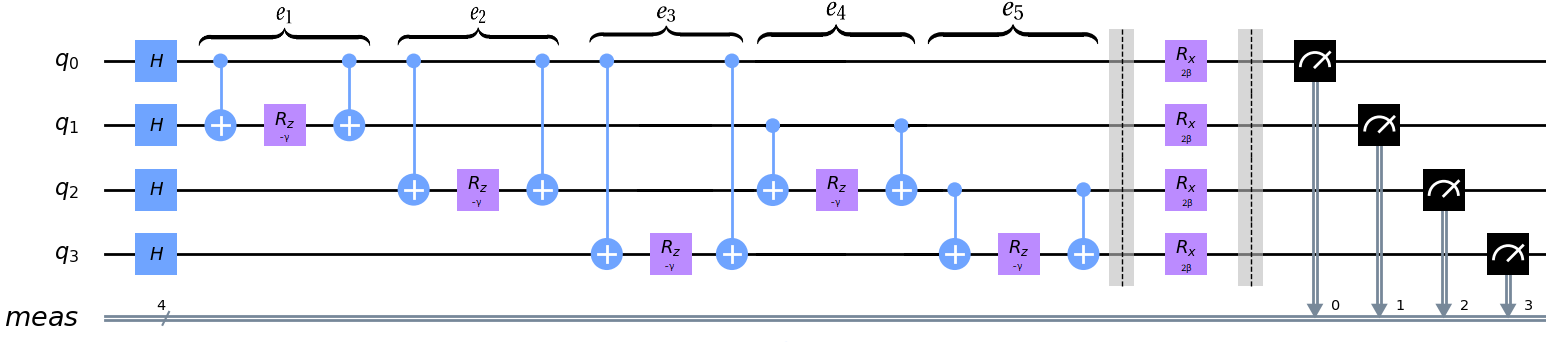
\includegraphics[width=\textwidth]{figures/circuit_diamond_edit2.png}
	\caption{Circuit for the diamond graph from Figure \ref{fig:graph-diamond} with parameters $\gamma$ and $\beta$ for the rotations using the cost and mixer Hamiltonians respectively. Every node in the graph is represented by a qubit, and the cost unitary can be implemented with two CNOT gates with a $R_z(-\gamma)$ gate in between for every edge in the graph, the relation to the graph edges is indicated with the braces. After the cost unitary, the mixer unitary is applied. This operator can be broken down into rotation gates $R_x(2\beta)$ applied to every qubit, or node. Finally, the system is measured in the computational basis.}
	\label{fig:circuit}
\end{figure}

\subsection{Maximizing the expectation value}
To give a sense of what it means to improve the expectation value of the cost function, several barplots are shown of the distribution resulting from sampling from three different states $|\gambe\rangle_{(p)}$ for $p=1,2,3$ after optimizing the angles for the diamond graph. As we can see, as we increase $p$ we are able to improve the expecation value and get good bit strings with high probability. In Section \ref{sec:optimal-parameters} I will go into more depth on how to determine an appropriate set of angles.

\begin{figure}[H]
	\centering
	\begin{subfigure}[t]{0.62\textwidth}
		\centering
		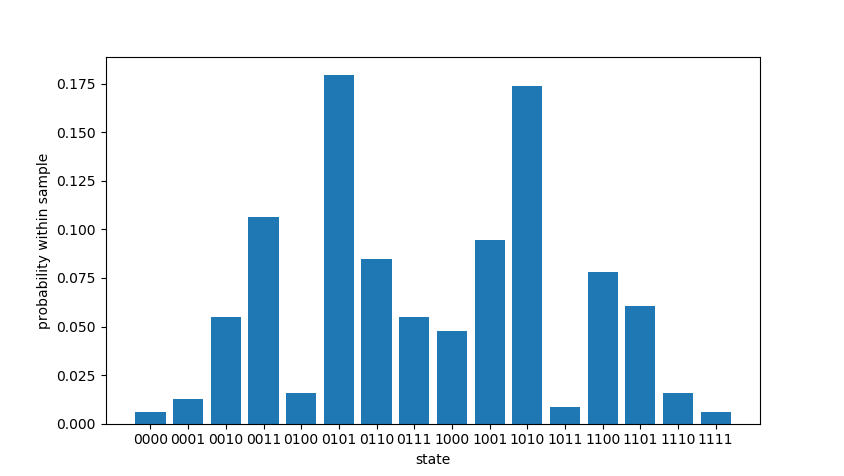
\includegraphics[width=\textwidth]{figures/histogram/diamond_p1.png}
		\captionsetup{justification=centering}
		\caption{$p=1$}
	\end{subfigure}
	\\
	\centering
	\begin{subfigure}[t]{0.62\textwidth}
		\centering
		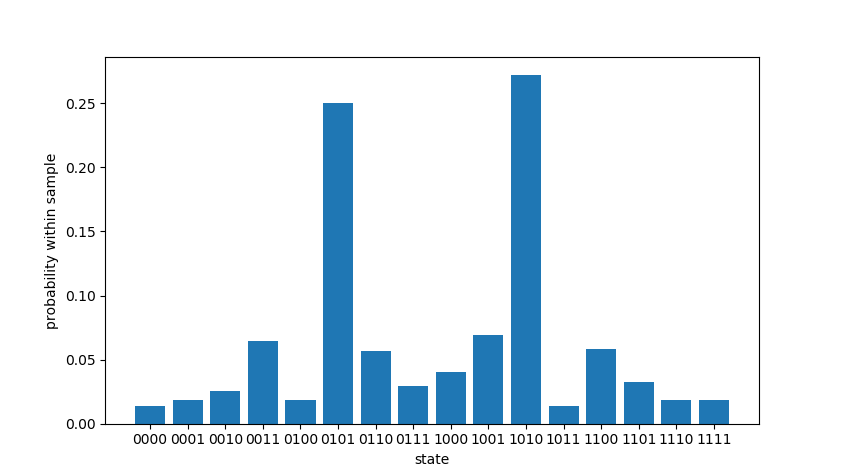
\includegraphics[width=\textwidth]{figures/histogram/diamond_p2.png}
		\captionsetup{justification=centering}
		\caption{$p=2$}
	\end{subfigure}
	\\
	\centering
	\begin{subfigure}[t]{0.62\textwidth}
		\centering
		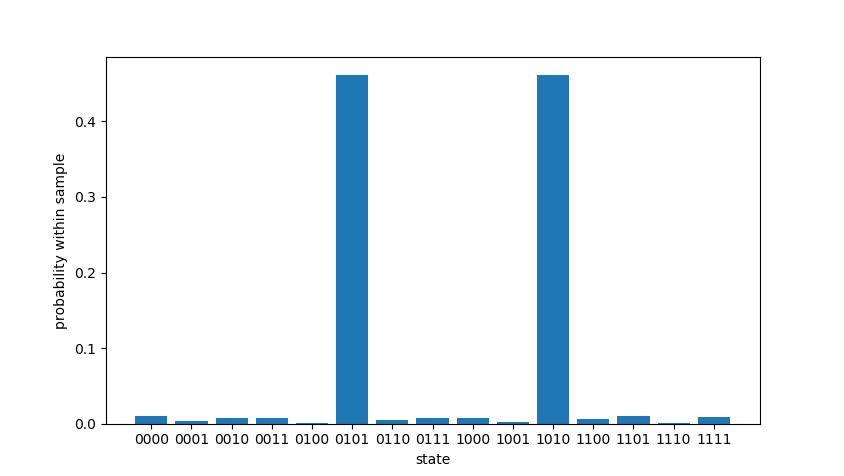
\includegraphics[width=\textwidth]{figures/histogram/diamond_p3.png}
		\captionsetup{justification=centering}
		\caption{$p=3$}
	\end{subfigure}
	\caption{Histograms of the distribution when sampling from the state $|\gambe\rangle_{(p)}$ for $p=1,2,3$ with $\vec{\gamma},\vec{\beta} \in \mathbb{R}^p$. The three sets of parameters are determined using BFGS optimization starting with a randomly chosen intial point. For these angles we have $F_1 = 3.24$, $F_2 = 3.39$, $F_3 = 3.87$. The order of the bits is $(0,1,2,3)$ where the labelling of the nodes is the same as in Figure \ref{fig:graph-diamond}. The optimal partitions are 0101 and 1010 with cutvalue 4.}
\end{figure}

\newpage

\subsection{Expectation landscapes}
To provide insight to what kind of expectation landscapes we might encounter, I will discuss the relevant features and symmetries that come into play in this section. In addition, I will show some expectation landscapes in the case of $p=1$.

For unweigthed graphs we find periodicity in the $\gamma$ direction. As mentioned in Section \ref{sec:general-setup}, this has to do with the fact that the cost Hamiltonian $H_C$ has integer eigenvalues, resulting in the identity
\begin{equation}
e^{2\pi i H_C} = I
\end{equation}
yielding a period of $2\pi$ in the $\gamma$ parameter in all layers. Moreover, there is $\mathbb{Z}_2$ symmetry to be exploited. This means that the partition $(S,\bar{S})$ is equivalent to the partition $(\bar{S},S)$, or in terms of bit strings a partition $10101$ is equivalent to $01010$ as the inversed labelling does not alter the value of a cut. Therefore if we apply $X^{\otimes n}$ to the state $|\gambe\rangle$ it does not change the expectation value $F_p = \langle H_C \rangle$. Note that the mixer unitary can be constructed with $R_x(2\beta)$ gates, but since $R_x(2\pi) \hat{=} X$ (up to global phase) we find a periodicity of $\pi$ in the $\beta$ parameter. Hence we can restrict $\beta \in [0,\pi)$ in general. Concluding, for unweighted graphs we have
\begin{equation}
\langle \gambe |H_C | \gambe \rangle = \langle \vec{\gamma} + 2\pi \vec{n}, \vec{\beta} + \pi\vec{m}|H_C|\vec{\gamma} + 2\pi \vec{n}, \vec{\beta} + \pi\vec{m}\rangle \qquad \vec{n},\vec{m} \in \mathbb{N}^p
\end{equation}
and for weighted graphs we have
\begin{equation}
\langle \gambe |H_C | \gambe \rangle = \langle \vec{\gamma}, \vec{\beta} + \pi\vec{m}|H_C|\vec{\gamma}, \vec{\beta} + \pi\vec{m}\rangle \qquad \vec{m} \in \mathbb{N}^p
\end{equation}

In Figures \ref{fig:landscapes-diamond} and \ref{fig:landscapes-butterfly} some examples of $F_1$ landscapes are shown. Remember that $F_1 = \langle \gamma, \beta | H_C | \gamma, \beta \rangle$ was defined to be the expectation value of the cost Hamiltonian. This means that if we repeatedly prepare the state $|\gamma,\beta\rangle$ and calculate the cut values, the average will be $F_1(\gamma,\beta)$. As explained, the aim is to seek values for $\gamma, \beta$ that maximize this quantity.
\begin{figure}[H]
	\begin{subfigure}[t]{0.42\textwidth}
		\centering
		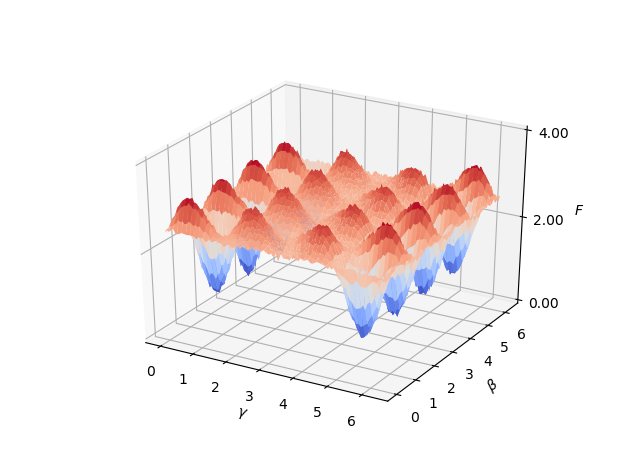
\includegraphics[width=\textwidth]{figures/landscape_new/diamond_3D.png}
		\caption{3D plot of $F_1$ for the unweighted diamond graph}
		\label{subfig:Diamond3D}
	\end{subfigure}%
	~ 
	\begin{subfigure}[t]{0.42\textwidth}
		\centering
		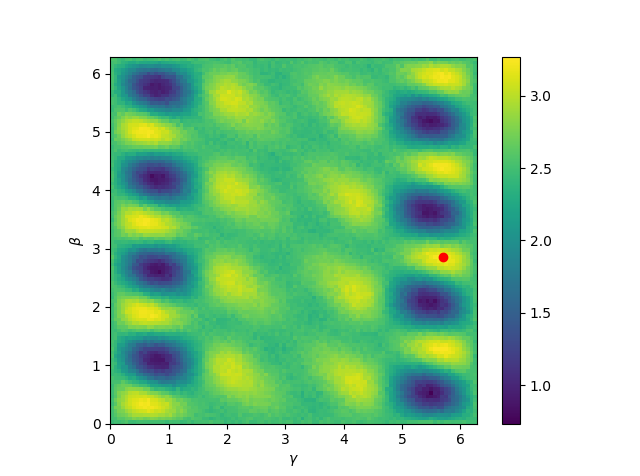
\includegraphics[width=\textwidth]{figures/landscape_new/diamond_imshow.png}
		\caption{Colorplot of $F_1$ for the unweighted diamond graph}
	\end{subfigure}
	\\
	\centering
	\begin{subfigure}[t]{0.45\textwidth}
		\centering
		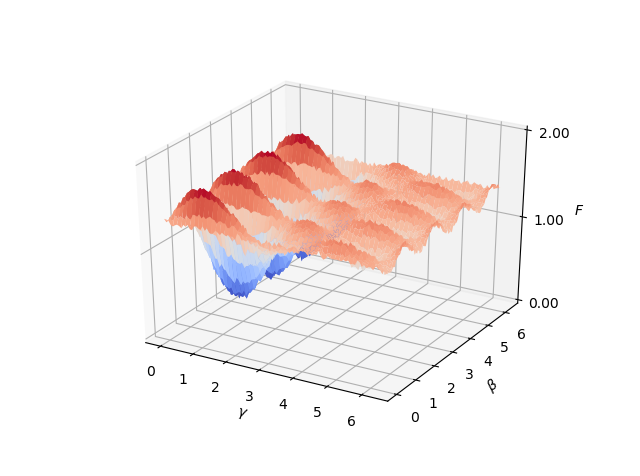
\includegraphics[width=\textwidth]{figures/landscape_new/diamond_weighted_3D.png}
		\caption{3D plot of $F_1$ for the weighted diamond graph.}
	\end{subfigure}%
	~ 
	\begin{subfigure}[t]{0.45\textwidth}
		\centering
		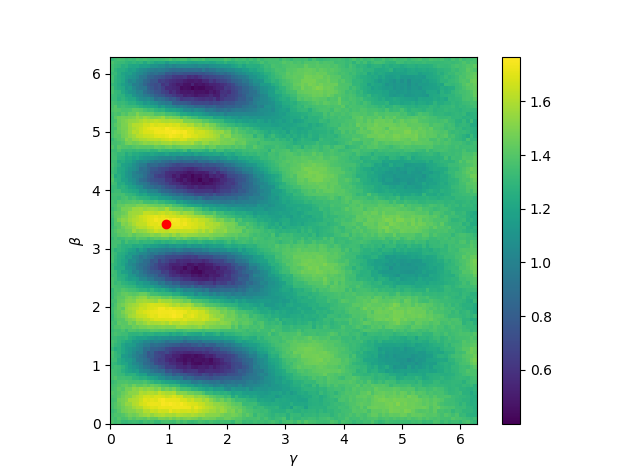
\includegraphics[width=\textwidth]{figures/landscape_new/diamond_weighted_imshow.png}
		\caption{Colorplot of $F_1$ for the weighted diamond graph}
	\end{subfigure}
	\caption{Landscapes of the expectation value $F_1$ for the unweighted (a), (b) and weighted (c), (d) Diamond graph (Figure \ref{fig:graph-diamond}) using a 3D plot and a colorplot respectively. The weights for the weighted graph were drawn from a uniform distribution $w_{ij} \sim U(0,1)$ for the weights of edges $\{i,j\} \in E$. In all plots both $\gamma, \beta$ range from $0$ to $2\pi$, divided into $100$ gridpoints. The expectation value $F_1 = \langle H_C\rangle$ is estimated using 1024 samples from the state $|\gamma, \beta \rangle$ at each gridpoint. The maximum is indicated by a red dot in the colorplots, note however that due to symmetries the actual optima are degenerate.}
	\label{fig:landscapes-diamond}
\end{figure}

\newpage
\begin{figure}[H]
	\centering
	\begin{subfigure}[t]{0.6\textwidth}
		\centering
		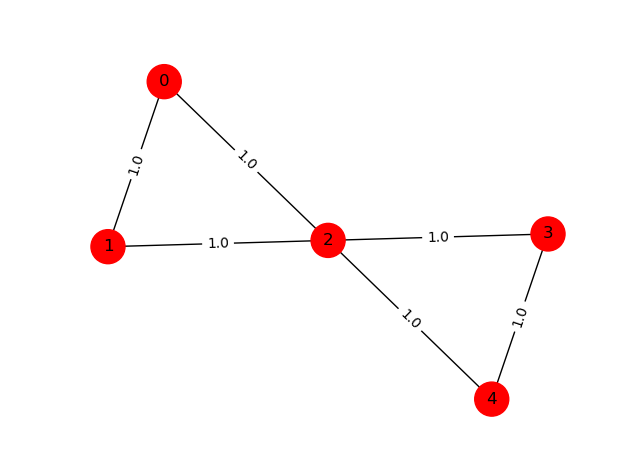
\includegraphics[width=\textwidth]{figures/butterfly-graph.png}
		\caption{Butterfly graph (unweighted)}
	\end{subfigure}%
	\\
	\centering
	\begin{subfigure}[t]{0.5\textwidth}
		\centering
		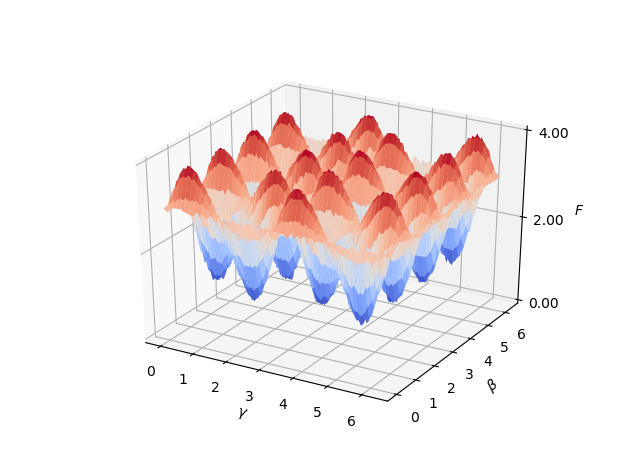
\includegraphics[width=\textwidth]{figures/landscape_new/butterfly_3D.png}
		\caption{3D plot of $F_1$ for the butterfly graph}
	\end{subfigure}%
	~ 
	\begin{subfigure}[t]{0.5\textwidth}
		\centering
		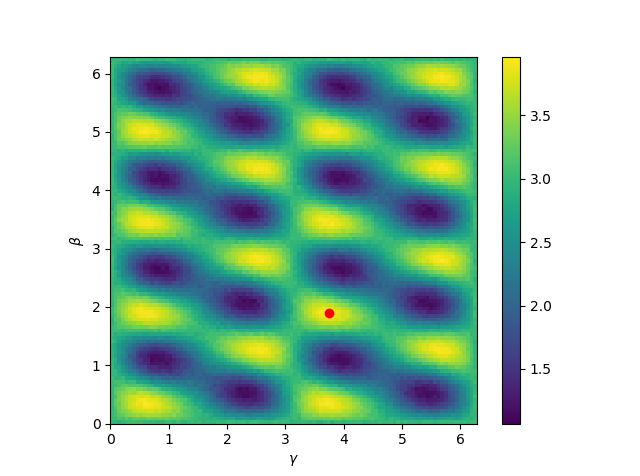
\includegraphics[width=\textwidth]{figures/landscape_new/butterfly_imshow.png}
		\caption{Colorplot of $F_1$ for the butterfly graph}
	\end{subfigure}
	\\
	\centering
	\begin{subfigure}[t]{0.5\textwidth}
	\centering
	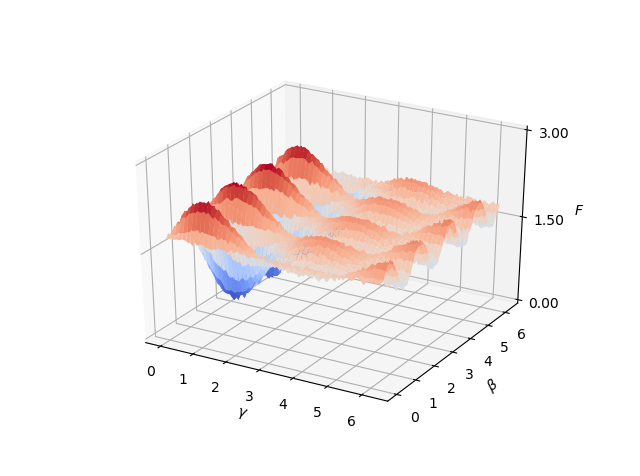
\includegraphics[width=\textwidth]{figures/landscape_new/butterfly_weighted_3D.png}
	\caption{3D plot of $F_1$ for the weighted butterfly graph}
	\end{subfigure}%
	~ 
	\begin{subfigure}[t]{0.5\textwidth}
	\centering
	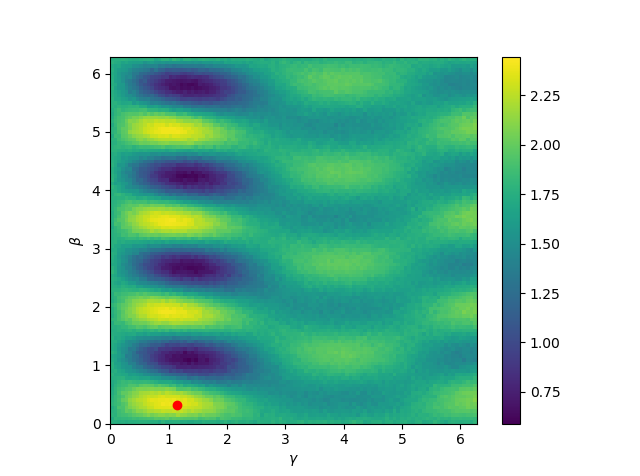
\includegraphics[width=\textwidth]{figures/landscape_new/butterfly_weighted_imshow.png}
	\caption{Colorplot of $F_1$ for the weighted butterfly graph}
	\end{subfigure}
	\caption{Landscapes of the expectation value $F_1$ for the unweighted (b), (c) and weighted (d), (e) Butterfly graph using a 3D plot and a colorplot respectively. The graph is visualized in (a). The weights for the weighted graph were drawn from a uniform distribution $w_{ij} \sim U(0,1)$ for the weights of edges $\{i,j\} \in E$. In all plots both $\gamma, \beta$ range from $0$ to $2\pi$, divided into $100$ gridpoints. The expectation value $F_1 = \langle H_C\rangle$ is estimated using 1024 samples from the state $|\gamma, \beta \rangle$ at each gridpoint. The maximum is indicated by a red dot in the colorplots, note however that due to symmetries the actual optima are degenerate.}
	\label{fig:landscapes-butterfly}
\end{figure}

\subsection{Adiabatic Theorem and the limit $p \to \infty$}
\label{subsec:adiabatic-theorem}
One of the main advantages of QAOA is the fact that its performance monotonically increases with $p$. This can be shown using the Adiabatic Theorem.
\begin{theorem}
	Suppose that the Hamiltonian of a system gradually changes from an initial form $H_i$ to some final form $H_f$. The Adiabatic Theorem states that if the system was initially in the $n$th eigenstate of $H_i$, then at the end of the process, the system will be in the $n$th eigenstate of $H_f$ \cite{Griffiths}. 
\end{theorem}

I would like to emphasize that this change has to be gradual, hence the name adiabatic (very much related to the same term in the context of thermodynamics). Using the Adiabatic Theorem it can be proven that as $p\to \infty$ the QAOA obtains the optimimal solution \cite{FGG14}
\begin{equation}
\lim_{p\to \infty} \max_{\gambe} F_p(\gambe) = \max_{\vec{x}} C(\vec{x})
\end{equation}
This configuration $\vec{x}$ corresponds to the is the groundstate energy of $-H_C$, where $H_C$ is the cost Hamiltonian defined in \eqref{eq:costHamiltonian}.

\subsection{Concentration}
\label{subsec:concentration}
While it is useful that we are guaranteed to improve the expectation ratio $F_p$ when increasing $p$, eventually we want to sample from the state $|\gambe\rangle$ to find an approximate solution. For this reason, it is desirable to know if the variance is bounded or not, since we would like to find bit strings with a cutvalue close to $F_p$ or better. This turns out to be the case. In the original paper \cite{FGG14}, it was proven that the variance is bounded by the following quantity.
\begin{equation}
\langle \vec{\gamma},\vec{\beta}|C^2|\vec{\gamma},\vec{\beta}\rangle - \langle \vec{\gamma},\vec{\beta}|C|\vec{\gamma},\vec{\beta}\rangle^2 \leq 2m \bigg[\frac{(v-1)^{2p+2}-1}{(v-1)-1}\bigg]
\label{eq:concentration}
\end{equation}
where $v$ is the maximum degree of the graph and $m$ the number of edges (or clauses). When $v$ and $p$ are taken to be constant, the standard deviation of $C(z)$ is at most of order $\sqrt{m}$. This has the advantageous implication that the sample mean of order $m^2$ values of $C(z)$ satisfies $|F_p(\vec{\gamma},\vec{\beta}) - C(z)| \leq 1$ with probability $1-\frac{1}{m}$, as we can estimate $F_p(\vec{\gamma},\vec{\beta})$ with a reasonable amount of samples.

\section{Finding optimal parameters}
\label{sec:optimal-parameters}
Several methods for finding optimal angles have been proposed in \cite{BBFGH18, Crooks18, ZWCPL18}. These methods include solving the problem analytically, doing a gridsearch of the parameter space \cite{FGG14}, using known optimization methods such as Nelder-Mead \cite{VBB17} or the Broyden–Fletcher–Goldfarb–Shanno algorithm \cite{ZWCPL18}, and even machine learning \cite{Crooks18, AAG20}. 

The first two approaches unfortunately do not scale well with $p$. Analytically solving for the optimal parameters requires evaluation of subgraphs of depth $p$. On the other hand, one could use a gridsearch by dividing the parameter space into $N$ points. This approach seems promising for fixed $p$, as the $F$-landscape is usually not jagged. To be precise, the partial derivatives of $F_p(\gambe)$ were shown to be bounded by $O(m^2+mn)$ \cite{FGG14}. There is one downside to this, to determine $2p$ parameters, we would have to estimate the expectation of the cost function $N^{2p}$ times, as this method is not at all efficient in $p$. There are also methods that use a variational approach, as will be discussed in the next section.

\subsection{Variational Quantum Eigensolver}
\label{sec:vqe}
The variational quantum eigensolver (VQE) is a quantum algorithm used to find the groundstate of a given Hamiltonian $H$ \cite{VQE, MRBA16}. It makes use of the variational principle which states that the expectation value of the Hamiltonian is always greater than or equal to the groundstate energy $E_0$  \cite{Griffiths}
\begin{equation}
\langle H \rangle \geq E_0
\end{equation}
for any state $|\psi\rangle$. The idea of VQE is to prepare a parameterized state $|\psi  (\vec{\theta}) \rangle$ that depends on some parameter set $\vec{\theta}$. This state is prepared using a unitary operator $U(\vec{\theta})$.
\begin{equation}
|\psi (\vec{\theta}) \rangle = U(\vec{\theta})|0\rangle
\label{eq:vqe-parametrized-unitary}
\end{equation} 
Using the variational principle, the ground state energy can be bound by $\langle \psi(\vec{\theta})|H|\psi(\vec{\theta})\rangle$. The actual goal is to find the optimal set $\vec{\theta}$ in order to prepare the groundstate, or a state that is close to it
\begin{equation}
\vec{\theta}_{\text{opt}} = \arg \min_{\vec{\theta}} \langle \psi(\vec{\theta})|H|\psi(\vec{\theta})\rangle
\end{equation}
The optimal parameters can be found with outer-loop classical optimization, see Figure \ref{fig:vqe}. Examples of possible methods include Nelder-Mead \cite{NelderMead}, the Broyden–Fletcher–Goldfarb–Shanno (BFGS) algorithm \cite{BFGS} or particle swarm optimization \cite{PSO1, PSO2}.

\begin{figure}[H]
	\centering
	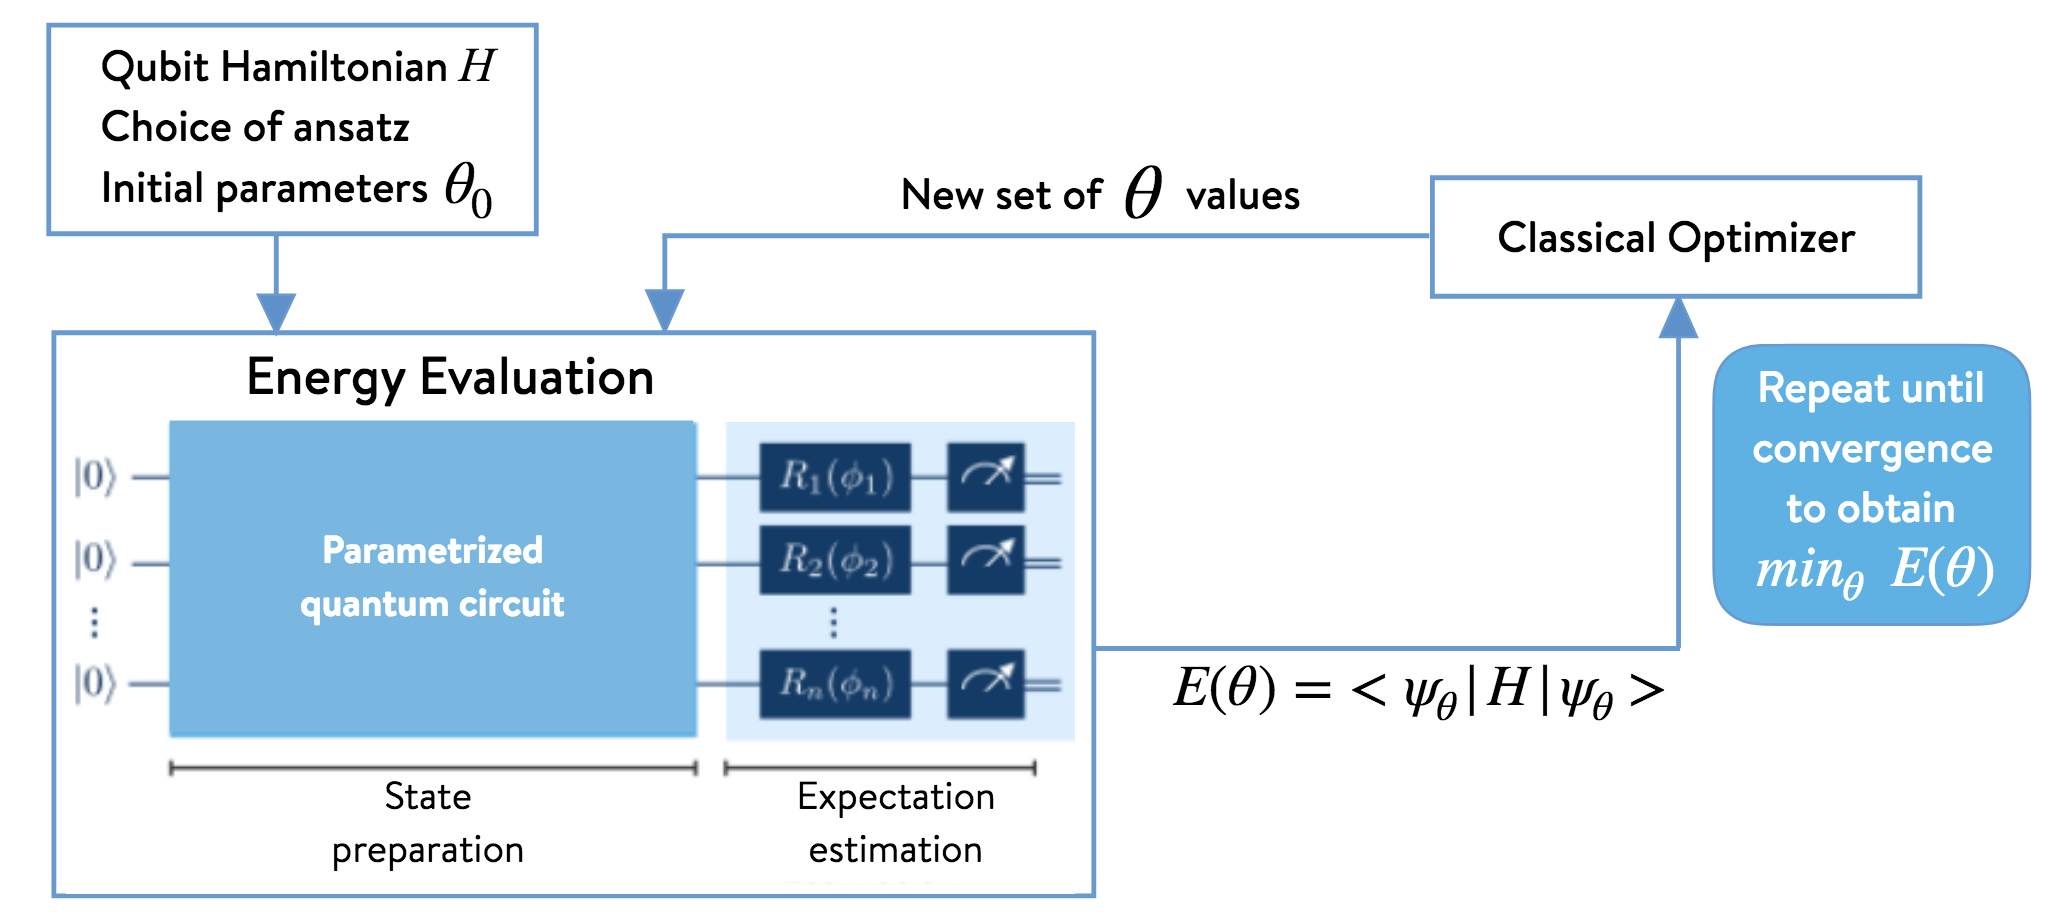
\includegraphics[scale=0.4]{figures/VQE_overview.png}
	\caption{Overview of the variational quantum eigensolver. A parametrized state is prepared after which the expectation value of the Hamiltonian is calculated classically. A classical optimization scheme determines a new set of parameters to be tried. This is repeated until convergence, or some other stopping criterium. Figure from \cite{vqe-figure}}
	\label{fig:vqe}
\end{figure}

It should be noted that the set of states that are possible to create is restricted by the structure of $U(\vec{\theta})$. Finding an appropriate ansatz operator $U(\vec{\theta})$ necessary to find the true groundstate can be difficult without prior knowledge of the problem.

Note that this is very similar to what we have to do in QAOA, namely finding the set of parameters $\gambe$ to maximize the expectation value of the cost Hamiltonian $H_C$, which is equivalent to minimizing the expectation value of $-H_C$
\begin{equation}
\vec{\gamma}_{\text{opt}}, \vec{\beta}_{\text{opt}} = \arg \min_{\vec{\gamma}, \vec{\beta}} \langle \gambe | -H_C | \gambe \rangle
\end{equation}
The form of the unitary in \eqref{eq:vqe-parametrized-unitary} in the case of QAOA is given by
\begin{equation}
	U(\vec{\gamma}, \vec{\beta}) = U(\beta_p, H_B)U(\gamma_p, H_C) \dots U(\beta_1, H_B)U(\gamma_1, H_C)H^{\otimes n}
\end{equation}

In fact, we can use VQE as a subroutine of QAOA for finding the optimal parameters \cite{ZWCPL18, Yao20}. An illustration hereof can be found in Figure \ref{fig:schematic-qaoa-vqe}. VQE is still an active field of research \cite{active-1,active-2,active-3}. It can be applied to QAOA, but also to areas such as chemistry where it is used for finding the groundstate energy of simple molecules \cite{VQE}.

In this thesis I will investigate one of the methods proposed in \cite{ZWCPL18} that makes use of the VQE subroutine. This method exploits certain patterns relating the optimal angles for different layers of the algorithm, reminiscent of the Quantum Adiabatic Algorithm. These patterns can be used to iteratively increase $p$, and determining an educated guess for the next QAOA layer from which an optimization routine is started for finding the local optimum. A more in depth discussion of these methods can be found in chapter \ref{chap:implementation}.
\begin{figure}[H]
	\centering
	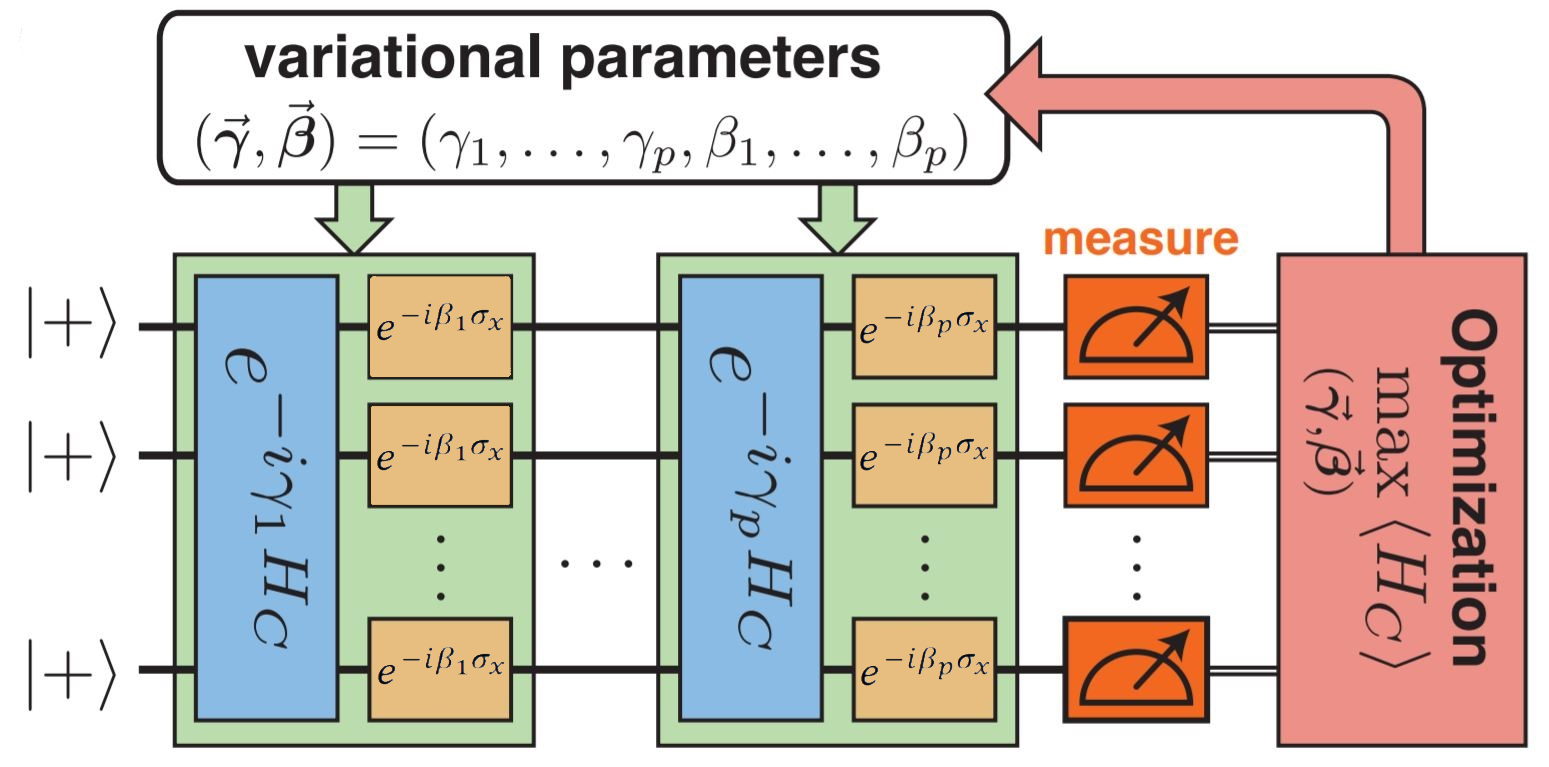
\includegraphics[width=0.7\textwidth]{figures/qaoa_idea_edit2.png}
	\caption{Schematic of a p-level Quantum Approximate Optimization Algorithm, making use of the variational approach to find optimal angles. The mixer hamiltonian is split into single qubit gates as explained in Subsection \ref{subsec:circuit}, in theory these can be applied in parallel. Adapted figure from \cite{ZWCPL18}.}
	\label{fig:schematic-qaoa-vqe}
\end{figure}

\section{Relation to the Quantum Adiabatic Algorithm}
The Quantum Adiabatic Algorithm, sometimes referred to as simply Quantum Annealing (QA), is a quantum algorithm for solving the satisfiability problem, proposed in \cite{FGGS2000} in 2000. The algorithm is based on adiabatic evolution and makes clever use of the adiabatic theorem presented in Section \ref{subsec:adiabatic-theorem}. The evolution of the quantum state is governed by the time-dependent Schr\"odinger equation
\begin{equation}
	i\frac{\partial }{\partial t} |\psi(t)\rangle = H(t)|\psi(t)\rangle
	\label{eq:schrodinger}
\end{equation}
where I included the factor $\hbar$ in $H(t)$. In QA we use a Hamiltonian $H(t)$ that interpolates between an initial Hamiltonian $H_i = H(0)$, whose ground state is easy to construct, and a final Hamiltonian $H_f = H(T)$, whose ground state encodes the satisfying assignment where $T$ is the total time of the evolution.  
\begin{equation}
H_i \xlongrightarrow{\text{time evolution}} H_f = \sum_{i=1}^m h_i
\end{equation}
Oftentimes, one uses an initial Hamiltonian $H_i$ with groundstate $|+\rangle^{\otimes n}$, which is easy to prepare on a quantum computer. A candidate for this initial Hamiltonian is $H_i = -(\sigma_x)^{\otimes n}$, with eigenvalues $1$ and $-1$ corresponding to the eigenstates $|-\rangle^{\otimes n}$ and $|+\rangle^{\otimes n}$, respectively. In the most general case we can represent the evolution using \cite{adiabatic-evolution1,adiabatic-evolution2}
\begin{equation}
H(t) = f(t)H_i + g(t)H_f
\label{eq:time-dependent hamiltonian}
\end{equation}
where $f(t)$ and g(t) are smooth functions of time with boundary conditions $f(0) = g(T) = 1$ and $f(T) = g(0) = 0$. One can simply choose a linear evolution, taking $f(t) = 1-t/T$ and $g(t) = t/T$, but other options are possible. 
Now consider the evolution of the state that is subject to this time-dependent Hamiltonian. The solution to \eqref{eq:schrodinger} defines the unitary operator $U(t,t_0)$ \cite{lecture-notes-evolution}
\begin{equation}
	|\psi(t)\rangle = U(t,t_0)|\psi(t_0)\rangle
	\label{eq:time-evolution}
\end{equation}
where $t_0$ is the initial time. Note that the operator works transitive in the sense that 
\begin{equation}
	U(t_2,t_0) = U(t_2,t_1)U(t_1,t_0)
\end{equation}
Combining \eqref{eq:schrodinger} and \eqref{eq:time-evolution}  yields the following expression
\begin{equation}
	i \frac{\partial }{\partial t} U(t,t_0)|\psi(t_0)\rangle = H(t)U(t,t_0) |\psi(t_0)\rangle
\end{equation}
and since the equation must hold for any (properly normalized) $|\psi(t)\rangle$ we find the following partial differential equation
\begin{equation}
	i \frac{\partial }{\partial t} U(t,t_0) = H(t)U(t,t_0)
	\label{eq:pde-evolution}
\end{equation}
subject to the initial condition $U(t_0,t_0) = I$ as $|\psi(t)\rangle = |\psi(t_0)\rangle$ if no time has passed.
Using a Taylor expansion and substituting the first order temporal derivative with \eqref{eq:pde-evolution} we can derive an expression for $U(t+\Delta t, t_0)$ up to second order in $\Delta t$
\begin{equation}
	U(t + \Delta t, t_0)= U(t,t_0) - i H(t)U(t,t_0)\Delta t + O(\Delta t^2)
\end{equation}
and so by using the initial condition we find
\begin{equation}
	U(t + \Delta t, t)= I - i H(t)\Delta t + O(\Delta t^2) = \exp\bigg\{-iH(t)\Delta t\bigg\} + O(\Delta t^2)
	\label{eq:taylor}
\end{equation}
where the latter equality holds because we are only concerned with terms up to $\Delta t$. Using this expression and transitivity, we can derive an expression for $U(t,t_0)$ for arbitrary timesteps $t-t_0$. We do this by dividing the time into very small steps $\epsilon = \frac{t-t_0}{N}$, so equation \eqref{eq:taylor} is approximately precise. This yield the following
\begin{equation}
	U(t,t_0) = \prod_{k=1}^N U(t_0 + k\epsilon, t_0 + (k-1)\epsilon) = \lim_{\epsilon \to 0}\prod_{k=1}^N \exp\bigg\{-i\epsilon H(t_0 + (k-1) \epsilon)\bigg\}
\end{equation}
If we can write this as an exponential of a sum, we might be able to rewrite it as an exponential of an integral when taking the limit $\epsilon \to 0$. However, we have to be wary of non-commutivity. A constant matrix always commutes with itself, but since we are considering a time-dependent matrix it might be the case that $H(t)$ does not commute with itself at different times. If $H(t_i)$ \emph{does} commute with $H(t_j)$ for every pair $t_i,t_j \in [t_0,t]$ we can write $U(t,t_0)$ as 
\begin{equation}
	U(t,t_0) = \exp \bigg\{-i\int_{t_0}^tH(t)\diff t\bigg\}, \qquad \text{ if } [H(t_i),H(t_j)] = 0 \forall t_i,t_j \in [t_0,t]
\end{equation}
Unfortunately, if $H(t_i)$ does \emph{not} commute with $H(t_j)$ for some pair $t_i,t_j \in [t_0,t]$, we need another approach. Instead, we need the \textbf{time-ordered exponential} to describe the evolution of the quantum state \cite{lecture-notes-evolution}. 

\begin{equation}
U(t,t_0) = \mathcal{T}e^{-i\int_{t_0}^t \diff \tau H(\tau)}
\end{equation}
where 
\begin{equation}
	\mathcal{T}e^{-i\int_{t_0}^t \diff \tau H(\tau)} = I + \sum_{k=1}^{\infty} \frac{(-i)^k}{k!} \int_{t_0}^t \diff t_1 \int_{t_0}^{t_1} \diff t_{2}\dots \int_{t_0}^{t_{n-1}} \diff t_n H(t_1)H(t_2)\dots H(t_n)
\end{equation}
This integral is hard to evaluate, however we can mitigate this using a the \textbf{Suzuki-Trotter} decomposition. In its most basic form we have \cite{Suzuki05}
\begin{equation}
	e^{Ax+Bx} = e^{Ax}e^{Bx} + O(x^2)
	\label{eq:suzuki-trotter}
\end{equation}
where $A$ and $B$ are arbitrary matrices and $x$ is some parameter. When applying the decomposition, one usually makes use of the relation
\begin{equation}
	\bigg(e^{\frac{x}{N}A}e^{\frac{x}{N}B}\bigg)^N = \underbrace{e^{\frac{x}{N}A}e^{\frac{x}{N}B}\dots e^{\frac{x}{N}A}e^{\frac{x}{N}B}}_{N \text{ times}} = e^{x(A+B) + \frac{1}{2}\frac{x^2}{N}[A,B] +O\big(\frac{x^3}{N^2}\big)}
\end{equation}
Note that we find $e^{(A+B)x} = (e^{\frac{x}{N}A}e^{\frac{x}{N}B})^N$ as $N$ tends to infinity. The Suzuki-Trotter expansion can be used to derive an approximation of the time-ordered exponential by discretizing the elapsed time $t-t_0$ into $N$ small intervals of length $\Delta t$ \cite{SZBW18}
\begin{equation}
	U(t,t_0) = \mathcal{T}e^{-i\int_{t_0}^t \diff \tau H(\tau)} \approx \prod_{k=0}^{N-1}\exp\bigg\{-iH(k\Delta t) \Delta t\bigg\} 
\end{equation}
Taking $H(t)$ from \eqref{eq:time-dependent hamiltonian} we have 
\begin{equation}
	\prod_{k=0}^{N-1}\exp\bigg\{-iH(k\Delta t) \Delta t\bigg\}  = \prod_{k=0}^{N-1}\exp\bigg\{-i\bigg(f(k\Delta t)H_i+ g(k\Delta t)H_f\bigg) \Delta t\bigg\}
\end{equation}
and using the approximation \eqref{eq:suzuki-trotter} we find 
\begin{equation}
	U(t,t_0) \approx \prod_{k=0}^{N-1}\exp\bigg\{-i\Delta tf(k\Delta t)H_i\bigg\}\exp\bigg\{-i\Delta t g(k\Delta t)H_f\bigg\}
\end{equation}
The approximation improves as $\Delta t$ gets smaller, and becomes exact when taking the limit $\Delta t \to 0$. Compare this with QAOA
\begin{equation}
	U_{QAOA}(\gambe) = \prod_{k=1}^p \exp\bigg\{-i\beta_k H_B\bigg\}\exp\bigg\{-i\gamma_k H_C\bigg\}
\end{equation}
 Seeing these parallels, one can consider QAOA as a discrete version of QA. Moreover, in Chapter \ref{chap:implementation} we will see that for the optimal parameter sets $\gambe$ we find that $\gamma_i$ monotonically increases and $\beta_i$ monotonically decreases, just like linear annealing in QA. These patterns were found both in \cite{ZWCPL18} and \cite{Crooks18} independently. A conceptual image of this relation is shown in Figure \ref{fig:QA-QAOA}

\begin{figure}[H]
	\centering
	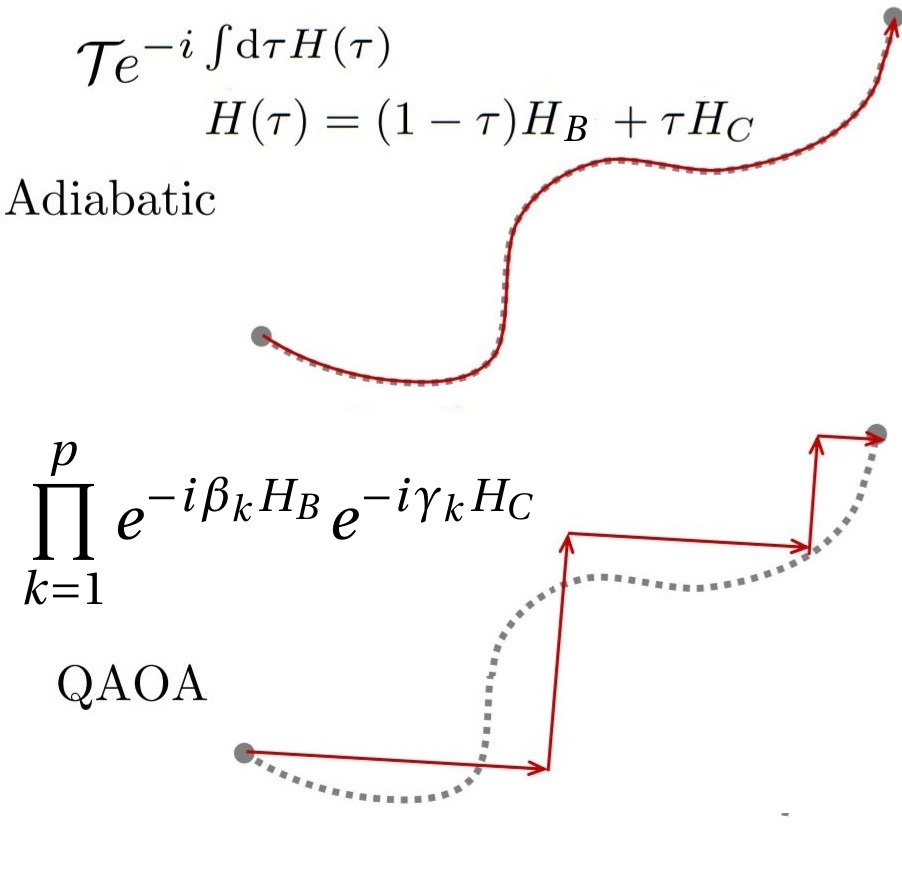
\includegraphics[width=0.4\textwidth]{figures/concept_relation_qaoa_and_qaa_edit.jpg}
	\caption{Conceptual analogy for comparing (bottom) QAOA
		to the (top) adiabatic algorithm with linear evolution as a path through state space. Adapted figure from \cite{VBB17}}
	\label{fig:QA-QAOA}
\end{figure}

In order to make sure that the system evolves to the ground state of the final Hamiltonian, the evolution must be gradual, hence the name adiabatic. Therefore, the evolution time $T$ must be long enough. It turns out that the time required for ``gradual'' evolution depends on the minimum energy gap $\Delta_{\min}$ between the groundstate and the first excited state during the evolution \cite{DMV02}.
\begin{equation}
	\Delta_{\min} \define \text{inf}\bigg\{\big|E_1(t)-E_0(t)\big|: t \in [0,T]\bigg\}
	\label{eq:spectral-gap}
\end{equation}
here $E_0(t)$ is the groundstate energy of $H(t)$, and similarly $E_1(t)$ is the energy of the first excited state. To guarantee that the system remains in the groundstate, the necessary run time of the algorithm should typically scale as $T = O(1/\Delta_{\min}^2)$ \cite{AL18, ZWCPL18}. In Figure \ref{fig:spectral-gap} an illustration of the minimum spectral gap is shown.
\begin{figure}[H]
	\centering
	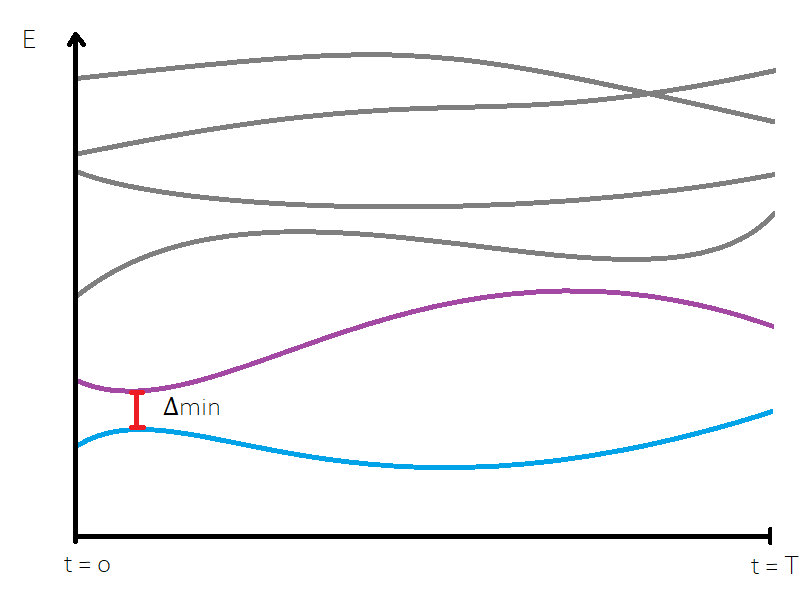
\includegraphics[width=0.5\textwidth]{figures/spectralGap.png}
	\caption{Example of an evolution of the eigenenergies of a time-dependent Hamiltonian $H(t)$. The {\color{cyan}blue} line represents the groundstate energy, and the {\color{purple}purple} line represents the energy of the first excited state. Here $\Delta_{\min}$ denotes the minimum (energy) distance between the groundstate and the first excited state of $H(t)$, as defined in \eqref{eq:spectral-gap}.}
	\label{fig:spectral-gap}
\end{figure}
A couple of years after the conception of the algorithm it turned out that for hard instances of 3SAT the gap between the lowest two energies can get exponentially close \cite{FGGN2005}. More precisely, it was shown that finding the minimum of a classical cost function whose domain is of size $N$, one needs the runtime to grow with at least the square root of $N$. In many combinatorial problems the domain size grows exponentially with the problem size $n$, so the approach is not efficient in $n$. The best one can hope for is Grover  (i.e. quadratic) speed-up, and thus the Adiabatic Algorithm does not disprove $P \neq NP$.



\chapter{Implementation}
\label{chap:implementation}

The QAOA algorithm is very reliant on finding appropriate angles $(\vec{\gamma},\vec{\beta})$ that favour good partitions and causes bad partitions to destructively interfere. One of the main obstacles to overcome is determining those optimal angles efficiently. In \cite{ZWCPL18} two methods were proposed to tackle this problem, INTERP and FOURIER that run in poly$(p)$ time. In this chapter, I will discuss the INTERP method together with the practical intricacies of implementing QAOA.
\\~\\
All the code developed for this thesis can be found on my GitHub repository: $\ $    \url{https://github.com/soosub/bep/} in the folder \code{Implementation/NewPlan}

\section{Patterns in the optimal parameters}

In order to improve upon current methods, extensive searches for globally optimal angles were conducted in \cite{ZWCPL18, Crooks18}  and independently found interesting results. After degeneracies were reduced from the parameter space, there were patterns to be found relating the optimal parameters for a particular graph at level $p$ to the optimal parameters at level $p+1$, as shown in Figure \ref{fig:patterns-zhou}.

\begin{figure}[H]
	\centering
	\begin{subfigure}[t]{0.5\textwidth}
		\centering
		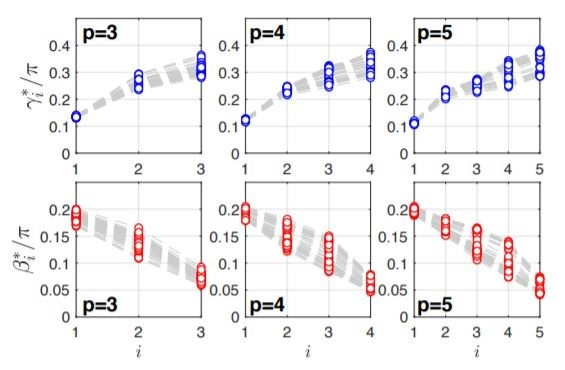
\includegraphics[width=\textwidth]{figures/patterns-u3R.jpg}
		\caption{Optimal parameters for unweighted 3-regular graphs}
	\end{subfigure}%
	~ 
	\begin{subfigure}[t]{0.5\textwidth}
		\centering
		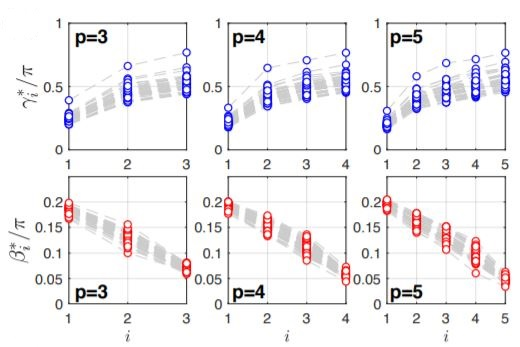
\includegraphics[width=\textwidth]{figures/patterns-w3R.jpg}
		\caption{Optimal parameters for weighted 3-regular graphs}
	\end{subfigure}
	\caption{ The parameter pattern visualized by plotting the optimal parameters of 40 instances of 16-vertex unweighted 3 regular graphs (a) and 16-vertex weighted 3 regular graphs (b), for $3 \leq p \leq 5$. The weights $w_{ij}$ in the weighted graphs were chosen from a uniform distribution $[0, 1]$. Each dashed line connects parameters for one particular graph instance. For each instance and each $p$, the classical BFGS optimization routine was used from $10^4$ random initial points, and the best parameters were kept. Figure and results from \cite{ZWCPL18}.}
	\label{fig:patterns-zhou}
\end{figure} 
\newpage
Independently, similar patterns were found on 10 node graphs in \cite{Crooks18}, see Figure \ref{fig:patterns-crooks}.

\begin{figure}[H]
	\centering
	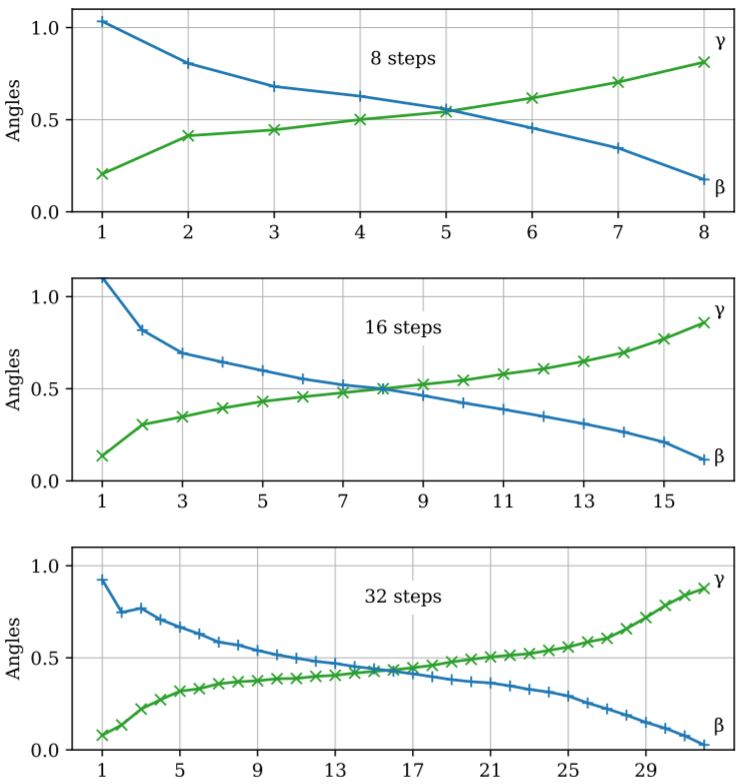
\includegraphics[scale=0.5]{figures/patterns-crooks.jpg}
	\caption{Examples of optimized parameters $(\vec{\beta}_{\text{opt}}, \vec{\gamma}_{\text{opt}})$ for Max-Cut QAOA on 10 node graphs, with 8, 16, and 32 QAOA	steps. The graph was chosen from the Erd\H{o}s-R\'enyi ensemble with edge probability 50\%.  When comparing with Figure \ref{fig:patterns-zhou}, there is a difference in the scaling of the $\beta_i$ parameters, this is because \cite{Crooks18} used the mixer Hamiltonian $H_B = \frac{1}{2}\sum_j \sigma_x^{(j)}$ whereas \cite{ZWCPL18} used the mixer Hamiltonian $H_B = \sum_j \sigma_x^{(j)}$, resulting in a factor 2 difference. Figure and results from \cite{Crooks18}.}
	\label{fig:patterns-crooks}
\end{figure}

As one can see from both results, $\gamma_i$ is a monotonically increasing sequence while $\beta_i$ is a monotonically decreasing sequence, for $i \in \{1, \dots p\}$. This is reminiscent of the Quantum Adiabatic Algorithm using a linear annealing schedule, where the initial Hamiltonian is turned off gradually while the final, or problem Hamiltonian is turned on \cite{AL18}. In addition, the optimal parameters found in $p$-level QAOA are very similar to the optimal parameters in the next level. This opens up the possibility of exploiting this relation in order to speed-up the parameter determination as will be discussed in Section \ref{sec:proposed-methods}.
	
\section{Proposed method by Zhou et al.}
\label{sec:proposed-methods}
In \cite{ZWCPL18}, it was suggested to use the patterns they found in order to enhance the search for optimal parameters. Two methods were proposed to achieve this, namely INTERP and FOURIER. Both methods require poly($p$) time, as opposed to, for example, gridsearch. The general idea in both methods is to use the optimal, or quasi-optimal angles at level $p$, and make an educated guess for the initial point of the optimization routine for the next level $p+1$. In the next section I will focus on the INTERP method.

\subsection{INTERP}
INTERP uses linear interpolation to produce a good initial point $(\vec{\gamma},\vec{\beta})$ for optimising the QAOA parameters as one iteratively increases the level $p$

\begin{equation}
\Big[\vec{\gamma}_{(p+1)}^0\Big]_i = \frac{i-1}{p}\Big[\vec{\gamma}_{(p)}^L\Big]_{i-1} + \frac{p-i+1}{p}\Big[\vec{\gamma}_{(p)}^L\Big]_i
\end{equation}
\begin{equation}
\Big[\vec{\beta}_{(p+1)}^0\big]_i = \frac{i-1}{p}\Big[\vec{\beta}_{(p)}^L\Big]_{i-1} + \frac{p-i+1}{p}\Big[\vec{\beta}_{(p)}^L\Big]_i
\end{equation}
for $i = 1, 2, \dots, p+1$. Here, the superscript indicates either that the angle pertains to the local minimum, $L$, or that it is the initial point for the next optimization round. The subscript inside the brackets indicates the QAOA level, and the subscript outside the brackets indicates the array element. Since the notation might seem a bit daunting, consider the following example. Suppose we have a (local optimal) set $\vec{\gamma}^L_{(3)} = (\gamma_1, \gamma_2,\gamma_3)$ for $p=3$ found after some optimization routine. Then, we can find a good initial point $\vec{\gamma}^0_{(4)} = (\gamma_1^0, \gamma_2^0,\gamma_3^0, \gamma_4^0)$ using the INTERP method for $p=4$ using these parameters, see Figure \ref{fig:interp-example}.
\begin{figure}[H]
	\centering
	\begin{subfigure}[t]{0.45\textwidth}
	\centering
	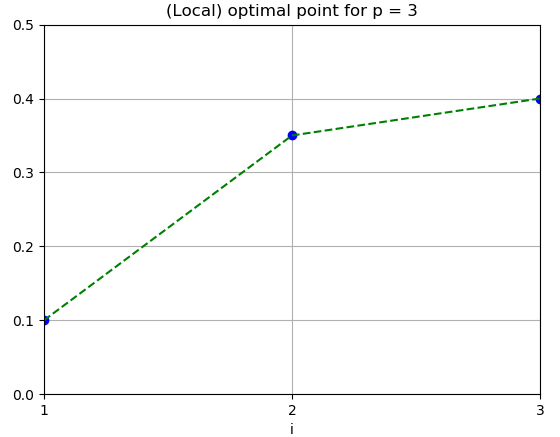
\includegraphics[width=\textwidth]{figures/heuristic_optimal_params.png}
	\end{subfigure}%
	~
	\begin{subfigure}[t]{0.45\textwidth}
		\centering
		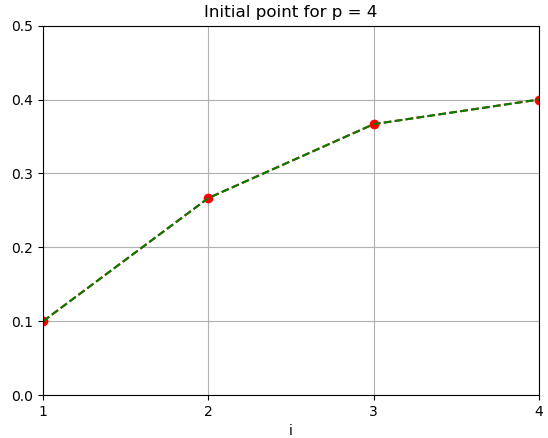
\includegraphics[width=\textwidth]{figures/heuristic_initial_params.png}
	\end{subfigure}%
	\caption{Illustration of INTERP method. The method uses the (local) optimal parameters to derive a good initial point for the optimization round of the next layer, using interpolation.}
	\label{fig:interp-example}
\end{figure}
Note that the parameters found using this interpolation are used as \emph{initial point} for the next round of optimization, so these are not directly the parameters used in the circuit. From this initial point we start another round of optimization to find a local optimum, that hopefully is also the global minimum or close to it. This is accomplished by considering the expectation value $\langle H_C \rangle$ as our objective function, which is estimated by sampling multiple times from the state $|\gambe\rangle$ and then calculating the corresponding objective value. When the next local minimum is found we use it to generate angles for the next $p$, and in this fashion we iteratively increase $p$ untill we are satisfied.

In some sense, it is flexible as one is not obliged to start from $p=1$, but can start at any level $p_{0}$ given an initial set of angles $\gamma_1, \beta_1 \dots \gamma_{p_{0}}, \beta_{p_{0}}$. For Max-Cut, it was recommended by Zhou to start from $p_0=1$ with $(\gamma, \beta) = (0.8,0.35)$ as an initial guess and work from there \cite{Zhou-email, genQAOA}. This is the approach I will use when producing the results in the next chapter. Alternatively, one could choose to do a gridsearch for the first layer requiring $O(1)$ function calls, and then proceed using INTERP.

%\section{Particle Swarm Optimization}
%In addition to the methods proposed in \cite{ZWCPL18}, I also tried out Particle Swarm Optimization (PSO) \cite{PSO1, PSO2} for parameter optimization. PSO is a gradient-free, evolutionary optimization approach that has been succesfully applied to many problems such as artificial neural network training, function optimization, and pattern classification \cite{Engelbrecht06,Poli08}. This was implemented using the package pySwarm \cite{pyswarm}. Applying PSO optimization to QAOA lead to some promising results in \cite{QAOA-pso}.

\section{Number of samples}
One algorithm design choice to consider is the number of samples from $|\gambe\rangle$ one needs when determining the final answer. Taking a constant number of samples would naturally lead to poor performance for large graphs, as the number of possible partitions grows exponentially with $n$. Another (naieve) option would be to take a certain fraction of the possible number of partitions, but asymtotically this would require $O(2^n)$ function calls. Ideally, we want to bound the number of samples by a polynomial function of $n$ and still get results close to or better than $F_p = \langle H_C \rangle$. It turns out we can. Remember from equation \eqref{eq:concentration} that the variance is bounded which implied that for fixed $p$ and $v$ the sample mean of order $m^2$ values of $C(\mathbf{z})$ will be in $[F_p(\gambe)-1,F_p(\gambe)+1]$ with probability $1 - \frac{1}{m}$ \cite{FGG14}. This means for reasonably large graphs ($m \gtrsim 10$), we can simply take $m^2$ samples and still find our estimate to be between $F_p \pm 1$ with reasonable probability. An illustration of the necessary $F_p$ evaluations as a fraction of the total number of partitions is shown in Figure \ref{fig:fraction}.

One thing to notice is that this impairs the applicability of QAOA for small graphs. The algorithm is inherently stochastic and so it requires multiple samples from the state $|\gambe\rangle$. When the number of samples required exceeds the number of possible partitions $2^n$ this nullifies the benefits of using the algorithm, even if we know good angles beforehand. Note that this fraction is based on \emph{one} evaluation of $F_p$. If, in addition, we still need to find good or optimal angles using classical optimization in the outer loop, then the number of necessary $F_p$-evaluations could diminish the usefulness of QAOA. Moreover, if one chooses to use a VQE subroutine for determining optimal angles it is likely that one would need more samples per function call since an unaccurate expectation estimate could restrain the effectiveness of the optimization when looking for (local) minima.

\begin{figure}[H]
	\centering
	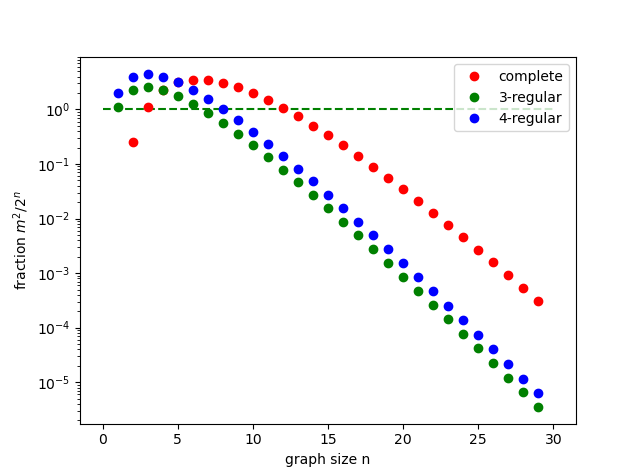
\includegraphics[width=0.58\textwidth]{figures/fraction.png}
	\caption{The ratio of necessary samples $m^2$ for finding a reasonalbe estimate for $\langle H_C \rangle$ and the total number of possible partitions $2^n$ as a function of the graph size $n$, here $m$ denotes the number of edges in the graph. With a reasonable estimate I mean that we find $F_{p, \text{sampled}}$ within 1 of the actual $F_p$ with a $1-\frac{1}{m}$ probability. The figure shows complete, 3-regular and  4-regular graphs. Note that for small complete graphs brute force approaches are superior to QAOA as one would need more samples then there are possible partitions to accurately estimate $F$.}
	\label{fig:fraction}
\end{figure}


\section{Implementation in Python}
\subsection{QAOA and Goemans-Williamson}
In order to examine the INTERP method, I implemented it using Python. For simulating the quantum circuit that is shown in Figure \ref{fig:schematic-qaoa}, I used pyQuil \cite{pyQuil}. pyQuil is a quantum instruction language developed at Rigetti Computing. It provides a way to simulate and compile quantum programs. The Quantum Virtual Machine (QVM) was used to run my experiments. Moreover, I made use of Grove, a collection of quantum algorithms built using the Rigetti Forest platform. Grove provides an implementation of QAOA using the VQE subroutine, on top of which I build the INTERP method. This was achieved by running the QAOA circuit for a certain set of initial angles to find a local minimum, which is illustrated in Figure \ref{fig:schematic-qaoa-vqe}. This local minimum was then used to calculate a new set of initial angles for the next QAOA layer according to the INTERP scheme. The optimizer used in the VQE subroutine was BFGS \cite{BFGS}. The quantum parts were simulated using the QVM and perfect qubits and full connectivity were assumed. The expectation $F_p$ was calculated during the optimization rounds using a fast method by dotting the wavefunction with the objective operator \cite{pyQuil}.

To benchmark the INTERP method to other QAOA methods, I also analyzed the performance of QAOA when starting from randomly chosen initial points, again with the Grove's QAOA class. I will abbreviate this method to pyQuil RI (randomly intialised), or simply RI. This means that for a given $p$, the optimization is simply started from $\vec{\gamma} = (\gamma_1,...,\gamma_p)$ and $\vec{\beta} = (\beta_1,...,\beta_p)$ with $\gamma_i$ drawn from a uniform distribution $U[0,2\pi]$ and $\beta_i$ from a uniform distribution $U[0,\pi]$. Again I used a BFGS optimizer in the VQE subroutine.

I used the implementation of the Goemans-Williamson algorithm from the package cvxgraphalgs. 

\subsection{Graphs}
The graphs that were analyzed were generated using the Python package networkx \cite{networkx}, a Python package for the creation, manipulation, and study of graphs and complex networks. These graphs include cyclic graphs, 3-regular graphs and weighted 3-regular graphs, and graphs from the Erd\"os-R\'enyi ensemble with edge probabilities 0.5, and 0.75. To make sure the experiments done are reproducable, I used seeds to keep track of the randomly generated graphs, the 3-regular graphs and the Erd\"os-R\'enyi graphs. For the regular graphs, I used a seed ranging from 0 to $N$, where $N$ is the number of graphs analyzed for that particular class of graphs. The same was done for the Erd\"os-R\'enyi (ER) graphs, however for small graphs and low edge probability there is a small probability that there are no edges in the graph. To circumvent this, I simply used the condition that the set of edges had to be non-empty, and if it were empty skip to the next seed.\\

Python version 3.7.7 was used. Relevant software and Python packages with corresponding versions are included in Appendix \ref{appendix:packages}.

\chapter{Results}
\label{chap:results}
As mentioned in the previous chapter, for evaluating the performance of the INTERP method I analyzed its performance on several types of graphs, namely cyclic graphs, 3-regular graphs and weighted 3-regular graphs. Additionally, graphs from the Erd\"os-R\'enyi ensemble were investigated with edge probabilities 0.5, and 0.75. As a figure of merit of the performance of QAOA approaches, I used the following quantity, as introduced in \cite{ZWCPL18}
\begin{equation}
	r = \frac{F_p(\gambe)}{C_{\max}}
\end{equation}
where $C_{\max}$ is the actual optimum. I will refer to the quantity $1-r$ as the \emph{fractional error}. As the outcome of Goemans-Williamson is inherently stochastic, I introduce the following quantity to compare the Goemans-Williamson on an equal footing as QAOA
\begin{equation}
	r_{GW}(k) = \frac{\frac{1}{k}\sum_i^kC_{GW,i}}{C_{\max}}
\end{equation}
where I take the average outcome of $k$ samples of $C_{GW}$. In the rest of this chapter I consider $k=10$.

The results from this chapter were obtained using the pyQuil INTERP method \cite{pyQuil-INTERP}, or simply called INTERP, unless stated otherwise. The BFGS optimizer was used for finding the locally optimal parameters $\gambe$, and by iteratively incrementing $p$ using INTERP starting from $p=1$ with parameters $(\gamma_0, \beta_0) = (0.8, 0.35)$. Degeneracies from time reversal symmetry $F_p(\gambe) = F_p(-\vec{\gamma},-\vec{\beta})$ were removed by taking $(\vec{\gamma},\vec{\beta})' = (-\vec{\gamma},-\vec{\beta})$ when $\gamma_i,\beta_i < 0$ for all $i$. Remarkably, for almost all sets of parameters found using INTERP, either all or no angles were found to be negative.

In the appendices the data is presented in more detail. This includes the parameter patterns in Appendix \ref{appendix:patterns}, the runtime of simulating the algorithm in Appendix \ref{appendix:runtime}, and the dependence of the fractional error on $p$ in Appendix \ref{appendix:fractional-error}.

\section{3-regular graphs}

The figure of merit $r$ as well as the fractional error, for 25 random instances of unweighted 3-regular graphs with 12 nodes, are plotted in Figure \ref{fig:Fp 3-regular 12-nodal}. Note that the expectation value $F_p$ asymptotically approaches the optimal objective value as we see that $r$ approaches 1 asymptotically. Results for the other graphs are included in Appendix \ref{appendix:fractional-error}.

\begin{figure}[H]
	\centering
	\begin{subfigure}[t]{0.48\textwidth}
		\centering
		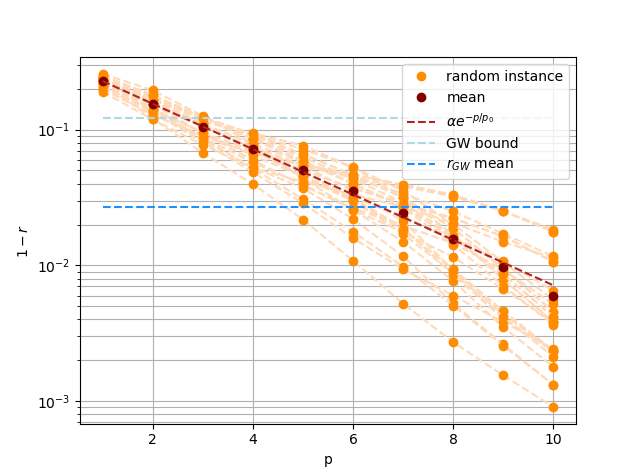
\includegraphics[width=\textwidth]{figures/interp/FOM_12_high_p.png}
		\caption{Fractional error $1-r$}
	\end{subfigure}
	\begin{subfigure}[t]{0.48\textwidth}
		\centering
		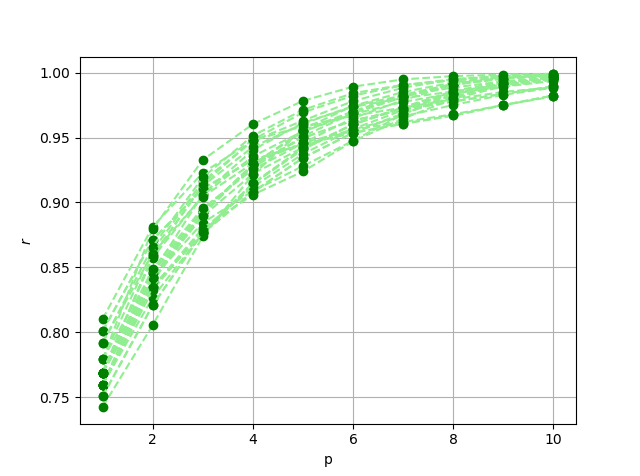
\includegraphics[width=\textwidth]{figures/interp/r_3-regular_12-nodal.png}
		\caption{Figure of merit $r$}
	\end{subfigure}%
	\caption{(a) The fractional error $1-r$ for the various randomly generated instances. A fit is included of the form $ae^{-p/p_0}$ where $\alpha = 0.334 \pm 0.003$ and $p_0 = 2.60 \pm 0.03$. (b) $r$ values after optimization for 25 instances of 12 nodal 3-regular graphs at various depths $p =  1, ... 10$. The angles were obtained by running the Grove QAOA method with the BFGS optimizer, by iteratively incrementing $p$ using INTERP starting from $(\gamma, \beta) = (0.8, 0.35)$.}
	\label{fig:Fp 3-regular 12-nodal}
\end{figure}

In Figure \ref{fig:pattern 3-regular 12-nodal} the patterns of (local) optimal parameters found with the pyQuil INTERP method.
\begin{figure}[H]
	\centering
	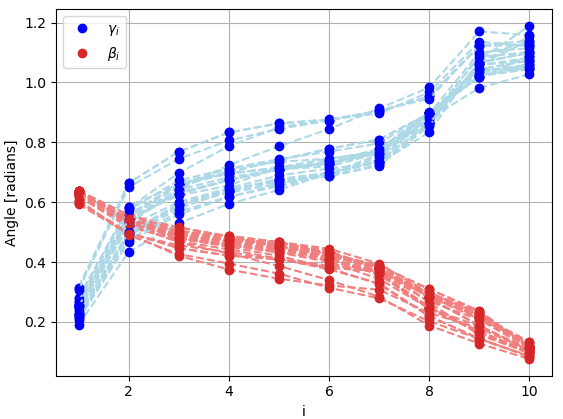
\includegraphics[width=0.5\textwidth]{figures/interp/pattern_3-regular_12-nodal.png}
	\caption{Patterns of the angles $\gambe$ for 25 instances of 12 nodal 3-regular graphs at depth $p=10$.}
	\label{fig:pattern 3-regular 12-nodal}
\end{figure}

These patterns are very reminiscent of the results found in earlier research \cite{Crooks18,ZWCPL18} in Figures \ref{fig:patterns-crooks} and \ref{fig:patterns-zhou} respectively. Not only does the monotonicity of the patterns coincide, the scaling is also very similar to both, taking the factor 2 in the mixer Hamiltonian into account from \cite{Crooks18}.  In Appendix \ref{appendix:patterns} the patterns are shown for different graph sizes $n$ and different classes of graphs. The monotonic patterns seem to be ubiquitous over the different classes of graphs, but there are certainly differences to be seen between the classes. Notable differences include the spread of the patterns for weighted graphs. For unweighted graphs the found parameters for different instances seem to concentrate. Moreover, the range of the patterns differs between the classes. For Erd\"os-R\'enyi graphs $\gamma$ typically varies from $\gamma_1 \approx 0.2$ to $\gamma_p \approx 0.7$ while for 3-regular unweighted graphs we typically find the $\gamma$-parameter ranging from $\gamma_1 \approx 0.4$ to $\gamma_p \approx 1$ and for 3-regular weighted graphs $\gamma_1 \approx 0.6$ to $\gamma_p \approx 1.6$.

In Figure \ref{fig:fom-exp-fit} the relation between $p$ and $r$ for weighted and unweighted 3-regular graphs is shown. As can be seen, for unweighted graphs the fractional error on average decreases exponentially with $p$. For weighted graphs we see a similar pattern, but for this class the fractional error decreases exponentially with the square root of $p$. Similar relations were found in \cite{ZWCPL18} for a similar method to INTERP, namely FOURIER.

\begin{figure}[H]
	\centering
	\begin{subfigure}[t]{0.65\textwidth}
		\centering
		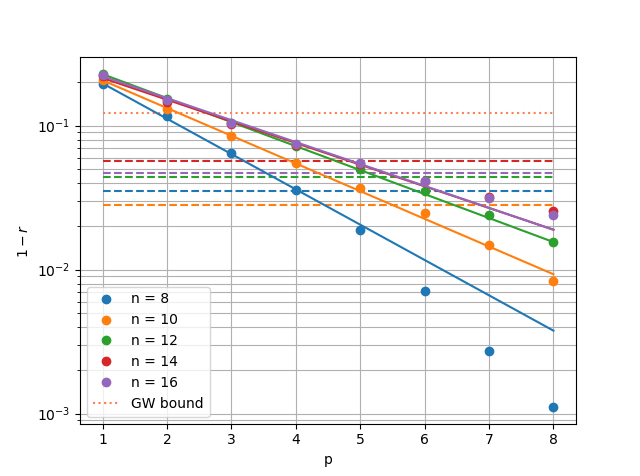
\includegraphics[width=\textwidth]{figures/interp/FOM_(unweighted)/system-size_unweighted_exp.png}
		\captionsetup{justification=centering}
		\caption{Unweighted 3-regular graphs}
	\end{subfigure}
	\\
	\centering
	\begin{subfigure}[t]{0.65\textwidth}
		\centering
		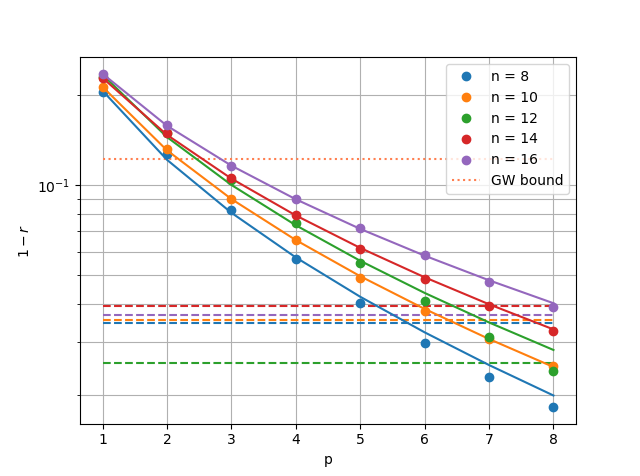
\includegraphics[width=\textwidth]{figures/interp/FOM_(weighted)/SQR/system-size_sqr.png}
		\captionsetup{justification=centering}
		\caption{Weighted 3-regular graphs}
	\end{subfigure}
	\caption{Dependence of $r$ on $n$ on 20 randomly generated unweighted 3-regular (a) and 20 randomly generated weighted 3-regular graphs (b) both using INTERP. For the unweighted graphs the model function $ae^{-p/p_0}$ was used, for the weighted graphs the model function $ae^{-\sqrt{p/p_0}}$ was used, these functions are shown with a solid lines. Moreover, the dashed horizontal lines indicate the average of $1-r_{GW}(10)$ for the 20 instances per nodal number. The coral coloured dotted line indicates $1-\rho$, where $\rho \approx 0.878$ is the approximation ratio of Goemans-Williamson.}
	\label{fig:fom-exp-fit}
\end{figure}
It is worth noting that from $p=6$ onwards QAOA outperforms Goemans-Williamson on all unweighted graphs when comparing the figures of merit $r$ and $r_{GW}$. For weighted 3-regular graphs we see that $p=8$ is not sufficient to outperform Goemans-Williamson on graphs of size 12 and 16. For this class of graph Goemans-Williamson often significantly performs better than the lower bound of $0.878$ in terms of the figure of merit $r_{GW}$. 

A graph of the dependence of $r$ on the number of nodes $n$ for unweighted 3-regular graphs is shown in Figure \ref{fig:r-n_dependence}. As we can see, generically $r$ decreases with $n$ for $p \geq 4$ for the INTERP method. For lower $p$ there seems to be some anomaly for 12 nodal graphs. In addition, we see that INTERP outperforms RI significantly for $p \geq 3$, especially on graphs with more nodes.


\begin{figure}[H]
	\begin{subfigure}[t]{0.62\textwidth}
		\centering
		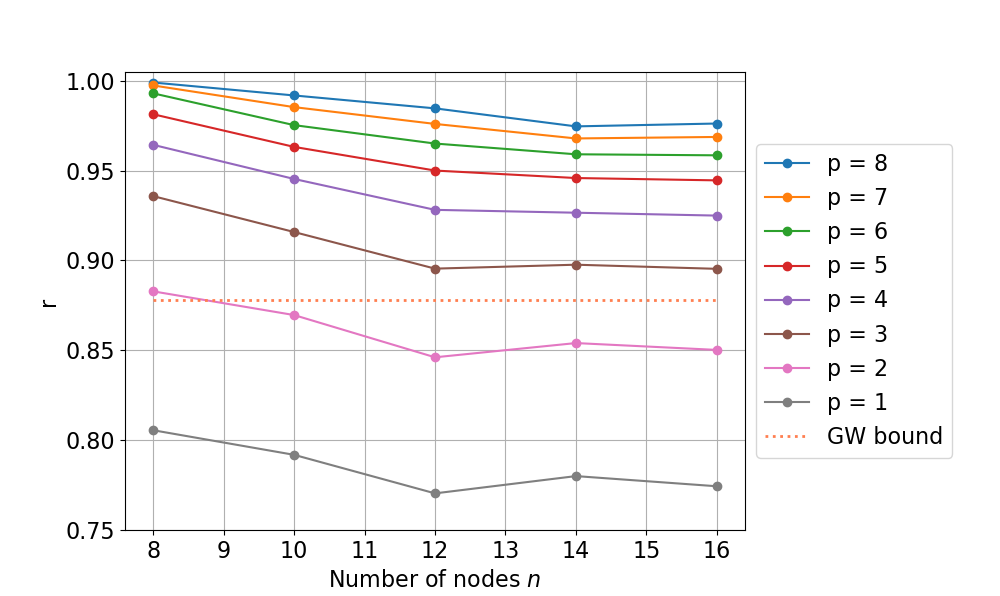
\includegraphics[width=0.85\textwidth]{figures/interp/INT_n_dependence.png}
		\captionsetup{justification=centering}
		\caption{INTERP $\qquad$ $\qquad$}
		\label{fig:r-n_dependence}
	\end{subfigure}
	\begin{subfigure}[t]{0.38\textwidth}
		\centering
		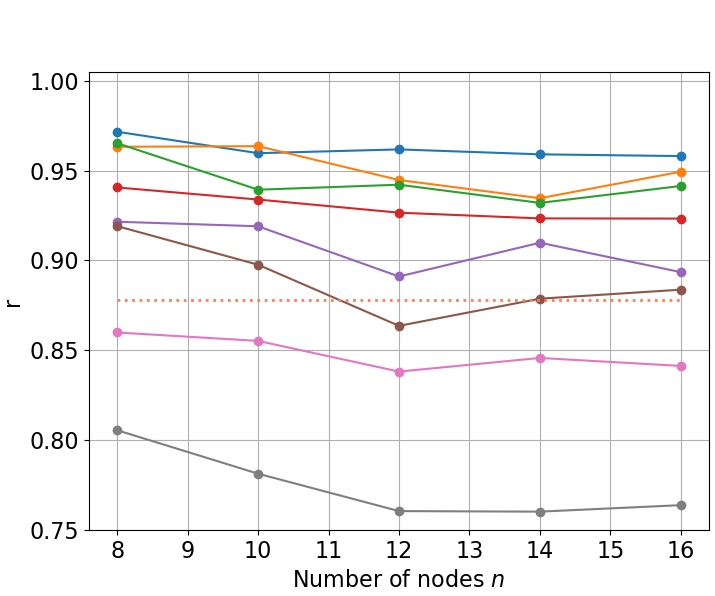
\includegraphics[width=\textwidth]{figures/RI/RI_n_dependence_3-regular_cut.png}
		\captionsetup{justification=centering}
		\caption{RI}
	\end{subfigure}
	\caption{Dependence of $r$ on $n$ on 20 randomly generated unweighted 3-regular graphs using both pyQuil INTERP (a) as well as pyQuil RI (b).  In both figures the lower bound of $0.878$ for the GW-algorithm is included.}
\end{figure}


The number of function evaluations necessary for parameter determination was also analyzed, see Figure \ref{fig:n_evals-3-regular}. The numerical results suggest that indeed the method is polynomial in $p$. For 3-regular graphs it was found that the necessary number of function evaluations was less than the number of function evaluations required for finding parameters for unweighted graphs.
\begin{figure}[H]
	\begin{subfigure}[t]{0.5\textwidth}
		\centering
		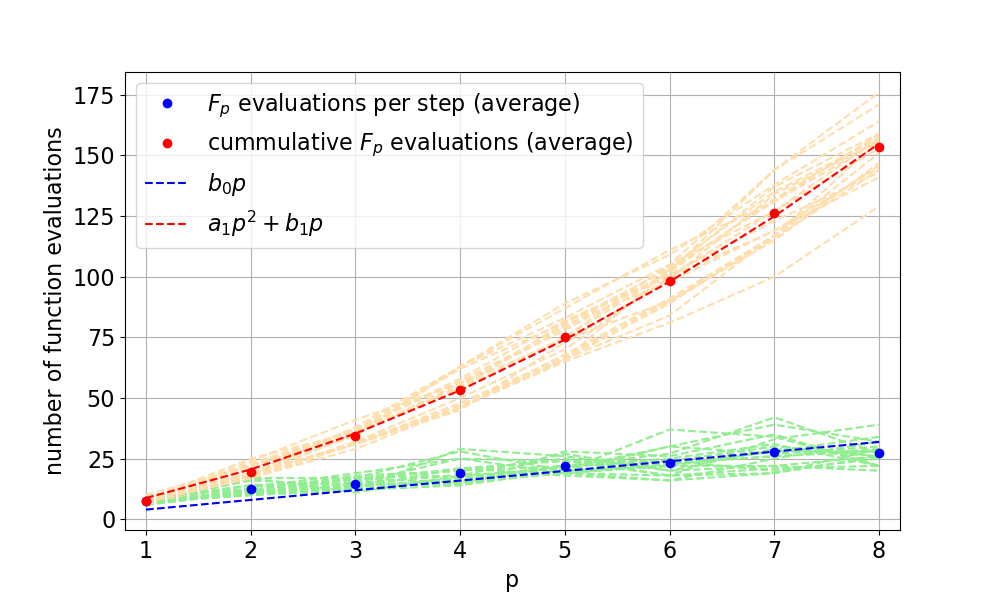
\includegraphics[width=\textwidth]{figures/interp/function_evaluations_16-nodal_unweighted.png}
		\captionsetup{justification=centering}
		\caption{Unweighted}
	\end{subfigure}
	\begin{subfigure}[t]{0.5\textwidth}
		\centering
		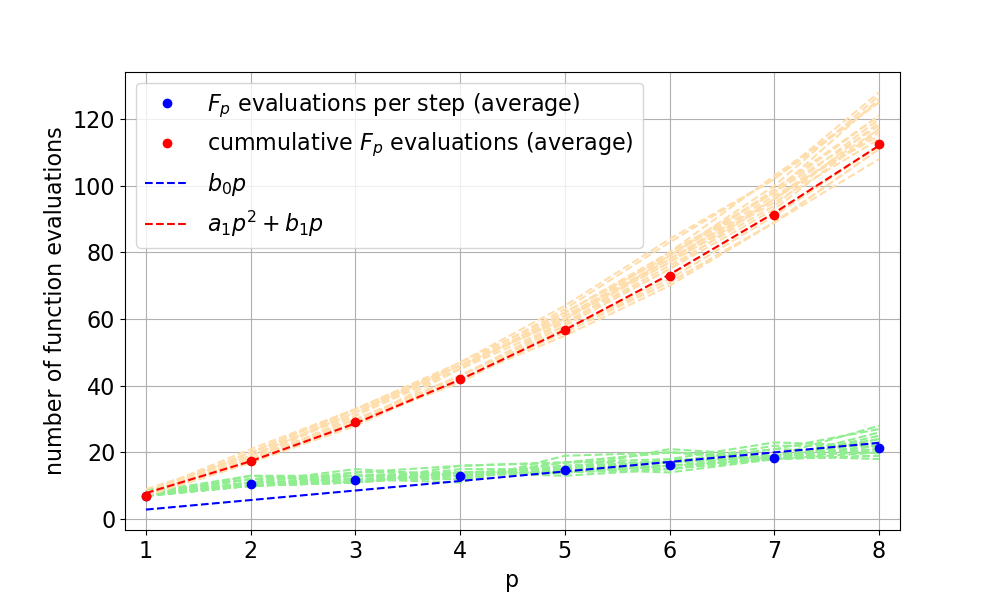
\includegraphics[width=\textwidth]{figures/interp/function_evaluations_16-nodal_weighted.png}
		\captionsetup{justification=centering}
		\caption{Weighted}
	\end{subfigure}
	\caption{Number of function evaluations necessary for parameter optimization in INTERP for 20 instances of 16-nodal 3-regular graphs. Both unweighted (a) and weighted (b). The fit parameters for the mean of the unweighted graphs are $b_0 = 4.0 \pm 0.2, a_1 = 1.52 \pm 0.05, b_1 = 7.2 \pm 0.3$. For the mean of the weighted graph the fitparameters found were $b_0 = 2.8 \pm 0.2, a_1 = 0.89 \pm 0.02, b_1 = 6.9 \pm 0.1$.}	
	\label{fig:n_evals-3-regular}
\end{figure}

\section{Erd\"os-R\'enyi graphs}
I also examined the performance of QAOA on Erd\"os-R\'enyi (ER) graphs with edge probability 0.50 and 0.75, abbreviated as ER-0.50 and ER-0.75 respectively. For graphs of this ensemble we find that the dependence of the fractional error acts similar to that of weighted 3-regular graphs as it also decreases exponentially with the square root of $p$, see Figure \ref{fig:fom-ER}.

\begin{figure}[H]
	\centering
	\begin{subfigure}[t]{0.48\textwidth}
		\centering
		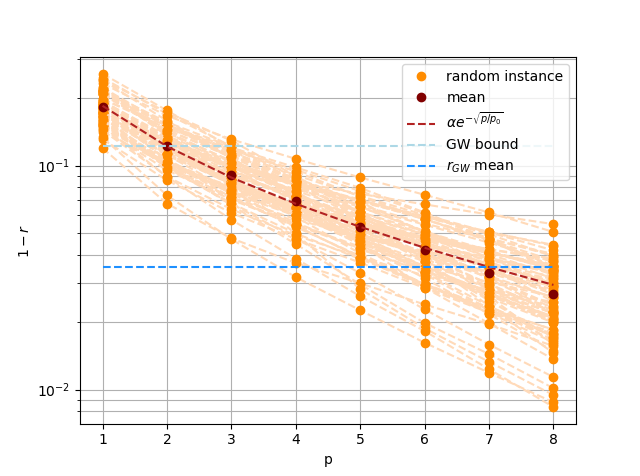
\includegraphics[width=\textwidth]{figures/interp/fom_er050.png}
		\caption{Fractional error $1-r$ for ER-0.50 graphs (20 instances). The fit parameters are $\alpha = 0.51 \pm 0.01$ and $p_0 = 0.99 \pm 0.03$.}
	\end{subfigure}%
	~
	\begin{subfigure}[t]{0.48\textwidth}
		\centering
		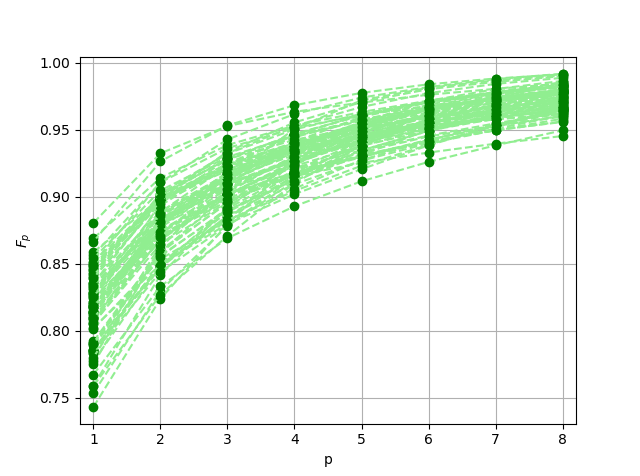
\includegraphics[width=\textwidth]{figures/interp/r_er050.png}
		\caption{Figure of merit $r$ for ER-0.50 graphs (20 instances).}
	\end{subfigure}%
	\\
	\begin{subfigure}[t]{0.48\textwidth}
		\centering
		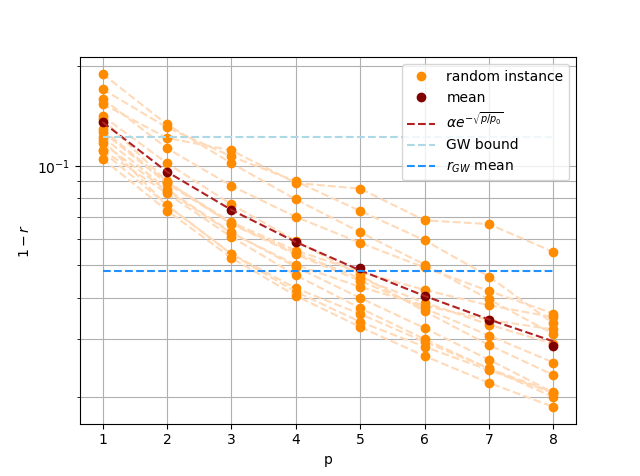
\includegraphics[width=\textwidth]{figures/interp/fom_er075.png}
		\caption{Fractional error $1-r$ for ER-0.75 graphs (10 instances). The fit parameters are $\alpha = 0.164 \pm 0.007$ and $p_0 = 4.1 \pm 0.3$}
	\end{subfigure}
	~
	\begin{subfigure}[t]{0.48\textwidth}
		\centering
		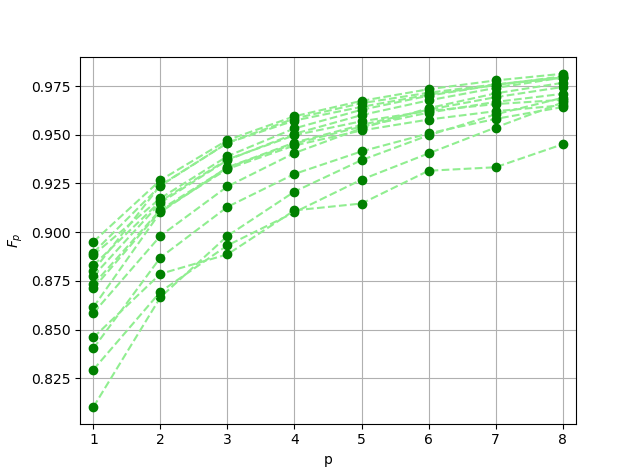
\includegraphics[width=\textwidth]{figures/interp/r_er075.png}
		\caption{Figure of merit $r$ for ER-0.75 graphs (10 instances)}
	\end{subfigure}%
	\caption{The fractional error and figure of merit for 12 nodal graphs of the Erd\"os-R\'enyi ensemble with edge probabilities 0.50 (a), (b) and 0.75 (c), (d) using the INTERP method for finding the parameters.}
	\label{fig:fom-ER}
\end{figure}

The dependence of $r$ on the number of nodes $n$ for the Erd\"os-R\'enyi graphs is shown in Figure \ref{fig:r-n_dependence_ER}. Again, we observe a general decreasing pattern in $r$ with $n$ from $p=4$ onwards. 

\begin{figure}[H]
	\begin{subfigure}[t]{0.6\textwidth}
		\centering
		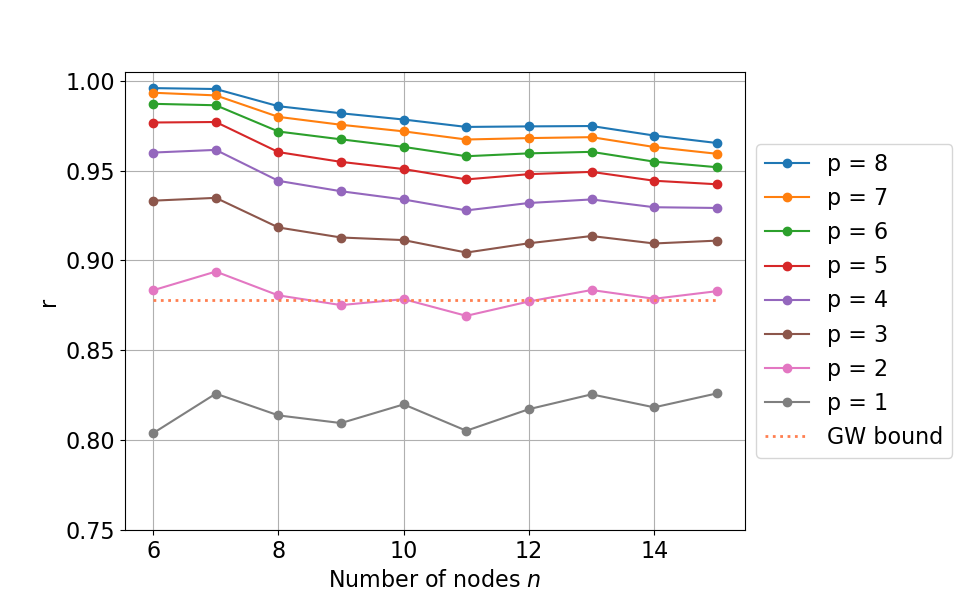
\includegraphics[width=0.85\textwidth]{figures/interp/INT_n_dependence_ER050.png}
		\captionsetup{justification=centering}
		\caption{ER-0.50}
		
	\end{subfigure}
	\begin{subfigure}[t]{0.4\textwidth}
		\centering
		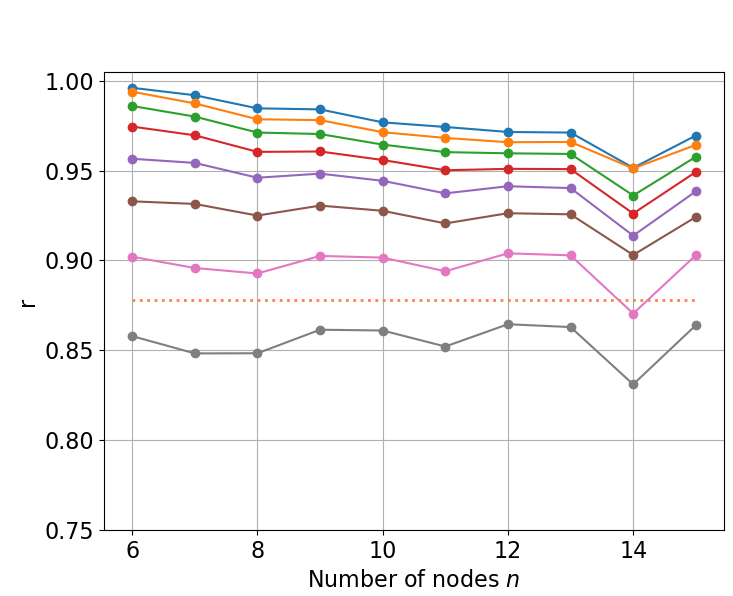
\includegraphics[width=\textwidth]{figures/interp/INT_n_dependence_ER075.png}
		\captionsetup{justification=centering}
		\caption{ER-0.75}
	\end{subfigure}
	\caption{Dependence of $r$ on $n$ on randomly generated unweighted ER graphs with edge probability 0.50 (a) as well 0.75 (b). In both figures the lower bound of $0.878$ for the GW-algorithm is included.}
	\label{fig:r-n_dependence_ER}
\end{figure}

The number of function evaluations for parameter determination is shown in figure \ref{fig:function-evaluations-ER}. We again observe that the method is polynomial in $p$. There seems to be no significant difference in the number of required function evaluations when comparing ER-0.50 and ER-0.75 graphs.
\begin{figure}[H]
	\centering
	\begin{subfigure}[t]{0.48\textwidth}
		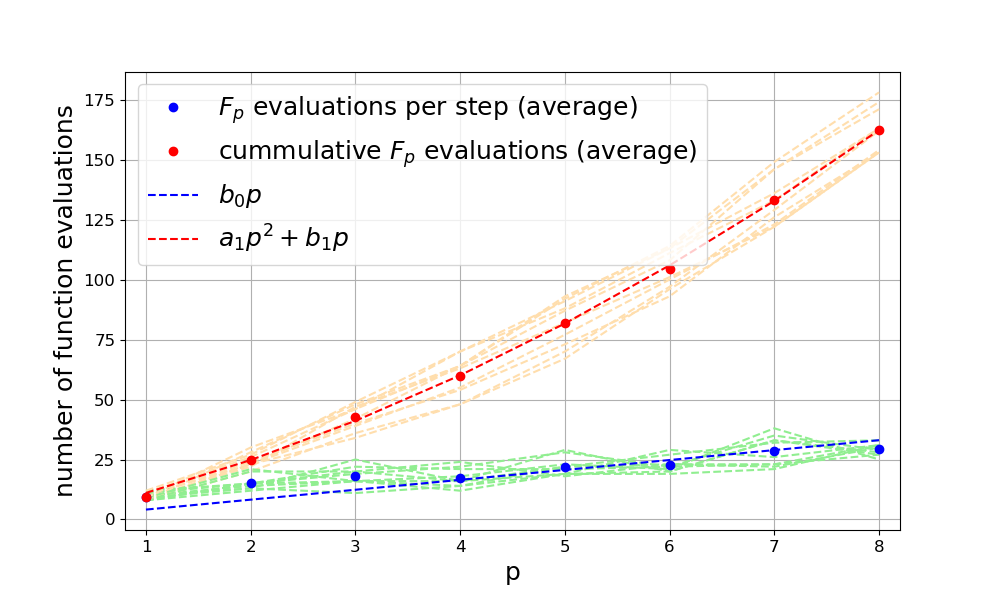
\includegraphics[width=\textwidth]{figures/interp/function_evaluations_15-nodal_ER050.png}
		\caption{15 nodal ER-0.50 graphs (20 instances)}
	\end{subfigure}
	\begin{subfigure}[t]{0.48\textwidth}
		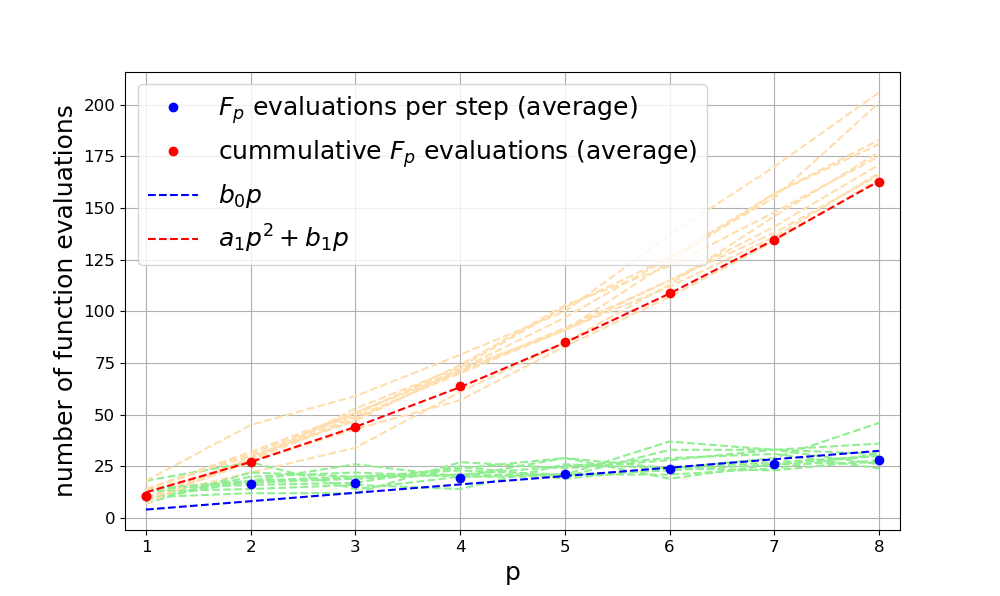
\includegraphics[width=\textwidth]{figures/interp/function_evaluations_15-nodal_ER075.png}
		\caption{15 nodal ER-0.75 graphs (10 instances)}
	\end{subfigure}
	\caption{Number of $F_p$ function evaluations necessary for the INTERP method to converge on ER graphs with 15 nodes. (a) 20 instances with edge probability 0.5 and fit parameters $b_0 = 4.1\pm0.3$ and $a_1=1.32 \pm 0.04, b_1 = 9.7\pm0.3$ (b) 10 instances with edge probability 0.75 and fit parameters $b_0 = 4.5\pm0.4$ and $a_1=1.25 \pm 0.03, b_1 = 12.4\pm0.2$. }
	\label{fig:function-evaluations-ER}
\end{figure}

\section{Cyclic graphs}
In the original QAOA paper \cite{FGG14}, an analytical expression for $F_p$ was derived by analyzing the contribution of subgraphs of size $p$ to the expectation value. As the graphs are cyclic, for $p<n/2$ there is only one type of subgraph, namely, a linear array of nodes. After maximizing the function numerically for $p=1,2,3,4,5$ and $6$ it was conjectured that for cyclic graphs one finds
\begin{equation}
\max_{\gambe}F_p = M_p = n\frac{2p+1}{2p+2}
\label{eq:cyclic-conjecture}
\end{equation}
for all $p < n/2$. To test this conjecture, I applied the pyQuil INTERP method to cyclic graphs. The $F_p$ values found by this method is shown in Figure \ref{fig:cyclic-conjecture}.

\begin{figure}[H]
	\centering
	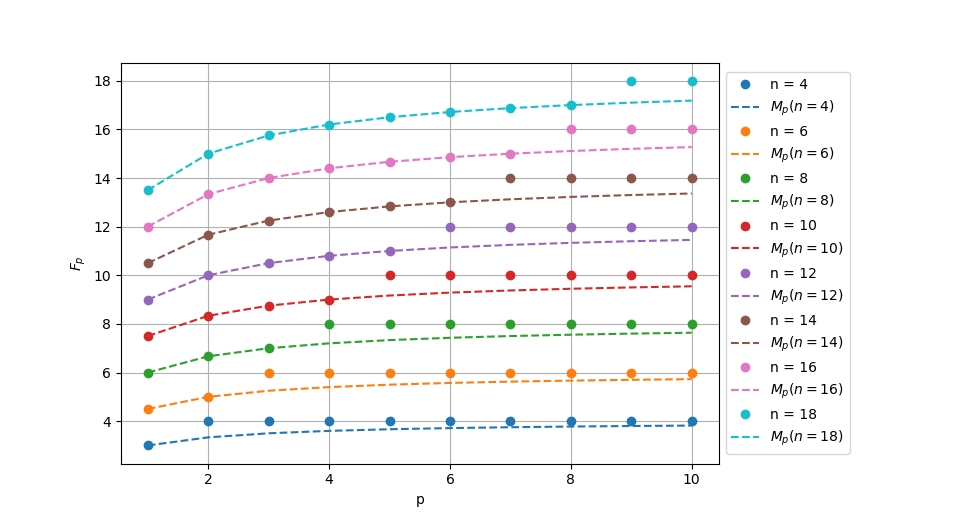
\includegraphics[width=0.9\textwidth]{figures/interp/cyclic_conjecture.png}
	\caption{The expectation value $F_p$ using the pyQuil INTERP method, for cyclic graphs with an even number of nodes $n$. The dots indicate the actual $F_p$ values from 1024 samples of the state. The dashed lines indicates the $M_p(n)$ values from Equation \eqref{eq:cyclic-conjecture} for various $n$ as a function of $p$.}
	\label{fig:cyclic-conjecture}
\end{figure}
It is noteworthy that for $p<n/2$ we indeed find that $M_p$ bounds $F_p$, and using the pyQuil INTERP method we attain that maximum $M_p$ with high precision. Beyond that, for $p \geq n/2$, the expectation value $F_p$ jumps to the facinity of the optimum value, namely $C_{\max} = n$, meaning $|\gambe\rangle$ is a groundstate of $-H_C$. 

In Figure \ref{fig:r-cyclic} the figure of merit $r$ is shown for cyclic graphs. As can be seen, there is a stark contrast between cyclic graphs with an even number of nodes, and an odd number of nodes. This is because the latter group has more partitions that are optimal as there has to be one neighbouring pair that are on the same side of the partition. Cyclic groups with an even number of nodes simply have one groundstate partitions, up to $\mathbb{Z}_2$ symmetry, namely an alternating bit string. This means that the groundstate of $-H_C$ has a higher degeneracy and thus the parametrized state $|\gambe\rangle$ naturally overlaps more with the groundstate.

\begin{figure}[H]
	\centering
	
	\begin{subfigure}[t]{0.5\textwidth}
		\centering
		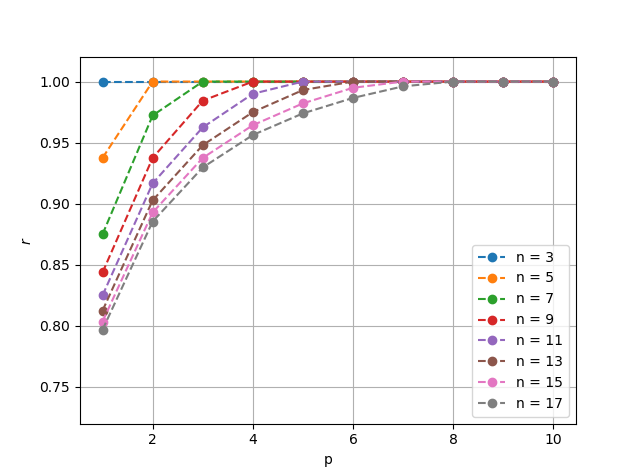
\includegraphics[width=\textwidth]{figures/interp/r_cyclic_odd.png}
		\caption{Odd $n$ where $C_{\max} = n-1$}
	\end{subfigure}%
	~ 
	\begin{subfigure}[t]{0.5\textwidth}
		\centering
		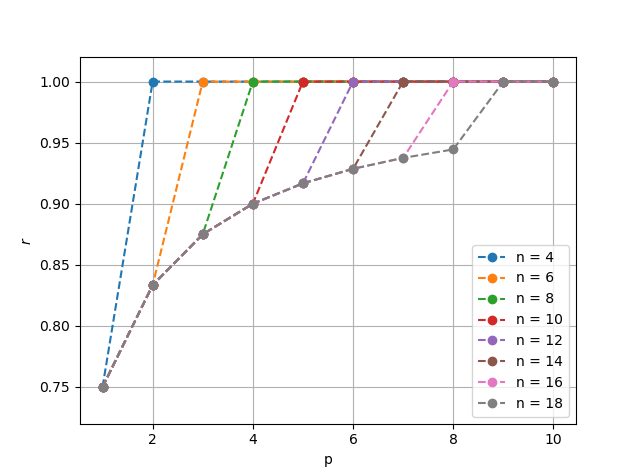
\includegraphics[width=\textwidth]{figures/interp/r_cyclic_even.png}
		\caption{Even $n$ where $C_{\max} = n$}
	\end{subfigure}
	\caption{Figure of merit $r$ for cyclic graphs of sizes $n= 2, \dots , 18$. The values for $F_p$ are acquired using the angles obtained using the pyQuil INTERP method.}
	\label{fig:r-cyclic}
\end{figure}


\chapter{Conclusions and Future Work}
\label{chap:conclusions}

The Quantum Approximate Optimization Algorithm (QAOA) is a variational quantum algorithm designed to solve combinatorial optimization problems that depends on $2p$ parameters. Due to its shallow depth it is relatively robust against errors and thus surpasses the need for error correction, making it an interesting algorithm to test on NISQ devices. One of the challenges for feasible use of the algorithm is the determination of suitable parameters. In this thesis I implemented and evaluated the INTERP method proposed by Zhou et al. \cite{ZWCPL18} that exploits similarities with the Quantum Adiabatic Algorithm in order to find quasi-optimal parameters in poly($p$) time. This was realized by benchmarking it against the classical Goemans-Williamson algorithm on a variety of graph classes, namely cyclic, 3-regular weighted and unweighted, and Erd\"os-R\'enyi graphs with edge probability 0.5 and 0.75. 

It was found that the depth $p$ required for surpassing the performance of Goemans-Williamson was dependent on the graph class. While only $p=2$ and in some cases $p=3$ was required for QAOA to surpass the approximation ratio of 0.878, the Goemans-Williamson algorithm is often able to do better. Accordingly, a different metric was chosen, namely $r_{GW}$ to compare Goemans-Williamson on equal footing with QAOA. For $p \gtrsim 6$ for unweighted 3-regular graphs, and $p \gtrsim 7$ for weighted 3-regular graphs, the QAOA algorithm using the INTERP method consistently outperforms the classical Goemans-Williamson algorithm in terms of this measure for small graphs with $n \lesssim 16$. Similarly, for Erd\"os-R\'enyi graphs $p \gtrsim 7$ was required for graphs with edge probability 0.5 and edge probability 0.75. However, this figure is also dependent on the graph size.

One important aspect of the algorithm is the amount of objective function calls required to find the parameters. It was found that this number is significant to the number of partitions for the small graphs analyzed in this thesis. This leads me to conclude that in practice one should prefer Goemans-Williamson over QAOA for small graphs when approximate solutions suffice.

The circuit implementing the algorithm applied to the Max-Cut problem requires only $O(n^2)$ gates by design, and the numeric results from this thesis suggested that the amount of function calls required for the outer loop classical optimization only grows polynomially in $p$, as was claimed in \cite{ZWCPL18}.  Therefore, the computational cost of finding quasi-optimal parameters using INTERP is expected to only grow polynomially in $n$ and $p$. For large graph sizes, the number of function calls will no longer be significant to the number of possible partitions as the latter grows exponentially with the problem size.

Moreover, it was found that monotonic patterns in the parameters were consistenly observed in all the classes of graphs that were investigated. One might wonder if this was enforced by the INTERP method itself. While it is possible that the found parameters are local optima, the results also show that the expectation value $F_p$ monotonically increases with $p$. This fact illustrates that the heuristic works well and offers a good alternative to gridsearches or randomly initialised optimization routines given the costly probing of the parameter space.
\\~\\
The work conducted in this thesis has also led to new questions. One of the main topics that requires further examination is whether or not it is possible to speed up the parameter determination. One idea that comes to mind is to use optimal parameters for one instance of a class of graphs, and use this to find good partitions. Closely related to this idea is to construct some function that closely resemebles the optimum pattern of a given graph class, and use this function to determine parameters, or start optimizing from this point to find local optimal parameters. Possibly, this could offer an advantage over an iterative method like INTERP that starts from a low $p_0$ and whose performance is greatly influenced by its initial point $(\vec{\gamma}_{(p_0)}, \vec{\beta}_{(p_0)})$. This approach could be aided with Machine Learning techniques to recognize relevant features of a given graph and its class.

Another topic of interest for future research is the implementation on actual quantum devices. As simulating the QAOA circuit on a classical device is not time-efficient, it is hard to get intuition for the time it takes on real quantum hardware combined with a classical computer. Because we are now approaching quantum devices with around 100 bits, it would be interesting to see if QAOA offers an advantage over classical algorithms for large problem sizes, as the exponential nature of many combinatorial optimization problems really becomes relevant for high $n$. A possible choke point for the speed of the algorithm would be the communication between the quantum computer and the classical computer. It would be interesting to see if hardware especially dedicated to these hybrid algorithms has advantageous beyond classical capability.

By extension, the problems that are forthcoming from real devices should also be investigated, such as the algorithm's resistance to error. Moreover, the mapping of the circuit onto the processor is subject to the processor constraints which might cause a loss in performance as real processors have limitted qubit connectivity. Furthermore, it should be investigated how the sampled average affects the speed of the classical optimization routine as it might cause problems due to the stochastic nature of the measurement outcomes.



%\begin{itemize}
%	\item One could wonder if the linear pattern was enforced by the INTERP method.
%	\item The number of samples and thus objective function calculations royally exceed the number possible partitions if starting INTERP from scratch, sometimes even 
%	\item Paper from Hastings
%	\item Paper hundreds of qubits
%	\item Integrated machine for VQE
%	\item Polynomial time?
%	\item when is QAOA faster, what are the applications
%	\item applications beyond Max-Cut \hl{It might be interesting to include some of this in the theory chapter (story about Max-E3-Lin2)}
%\end{itemize}



% bibliography
\bibliography{references}

% Appendices
\appendix % Use letters for the chapter numbers of the appendices.
\chapter{Parameter patterns}
\label{appendix:patterns}
\begin{figure}[H]
	\centering
	\begin{subfigure}[t]{0.7\textwidth}
		\centering
		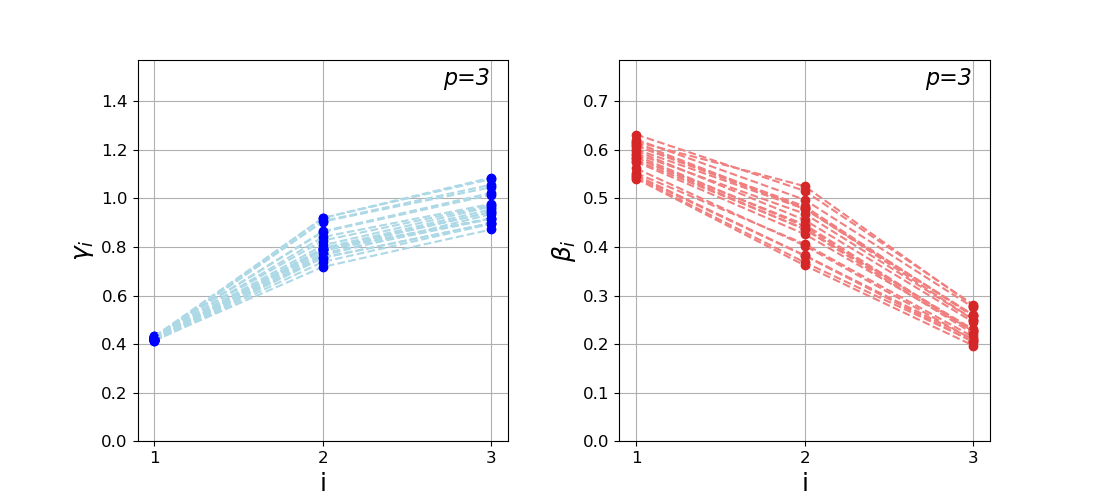
\includegraphics[width=\textwidth]{figures/interp/patterns/pattern_16-nodal_p-3.png}
	\end{subfigure}
	\\
	\centering
	\begin{subfigure}[t]{0.7\textwidth}
		\centering
		\includegraphics[width=\textwidth]{figures/interp/patterns/pattern_16-nodal_p-4.png}
	\end{subfigure}
	\\
	\centering
	\begin{subfigure}[t]{0.7\textwidth}
		\centering
		\includegraphics[width=\textwidth]{figures/interp/patterns/pattern_16-nodal_p-5.png}
	\end{subfigure}
	\caption{Quasi-optimal parameters $(\gambe)$ found using the pyQuil INTERP method for 20 instances of 3-regular unweighted graphs with 16 nodes for $p = 3, 4, 5$.}
	\label{fig:appendix-patterns-16-nodal}
\end{figure}

\newpage
\begin{figure}[H]
	\centering
	\begin{subfigure}[t]{0.7\textwidth}
		\centering
		\includegraphics[width=\textwidth]{figures/interp/patterns/pattern_16-nodal_p-3_weighted.png}
	\end{subfigure}
	\\
	\centering
	\begin{subfigure}[t]{0.7\textwidth}
		\centering
		\includegraphics[width=\textwidth]{figures/interp/patterns/pattern_16-nodal_p-4_weighted.png}
	\end{subfigure}
	\\
	\centering
	\begin{subfigure}[t]{0.7\textwidth}
		\centering
		\includegraphics[width=\textwidth]{figures/interp/patterns/pattern_16-nodal_p-5_weighted.png}
	\end{subfigure}
	\\
	\centering
	\begin{subfigure}[t]{0.7\textwidth}
		\centering
		\includegraphics[width=\textwidth]{figures/interp/patterns/pattern_16-nodal_p-8_weighted.png}
	\end{subfigure}
	\caption{Quasi-optimal parameters $(\gambe)$ found using the pyQuil INTERP method for 20 instances of 3-regular weighted graphs with 16 nodes for $p = 3, 4, 5$ and $8$}
	\label{fig:appendix-patterns-12-nodal-3-regular}
\end{figure}

\newpage
\begin{figure}[H]
	\centering
	\begin{subfigure}[t]{0.7\textwidth}
		\centering
		\includegraphics[width=\textwidth]{figures/interp/patterns/pattern_12-nodal_ER050_p-3.png}
	\end{subfigure}
	\\
	\centering
	\begin{subfigure}[t]{0.7\textwidth}
		\centering
		\includegraphics[width=\textwidth]{figures/interp/patterns/pattern_12-nodal_ER050_p-4.png}
	\end{subfigure}
	\\
	\centering
	\begin{subfigure}[t]{0.7\textwidth}
		\centering
		\includegraphics[width=\textwidth]{figures/interp/patterns/pattern_12-nodal_ER050_p-5.png}
	\end{subfigure}
	\\
	\centering
	\begin{subfigure}[t]{0.7\textwidth}
		\centering
		\includegraphics[width=\textwidth]{figures/interp/patterns/pattern_12-nodal_ER050_p-8.png}
	\end{subfigure}
	\caption{Quasi-optimal parameters $(\gambe)$ found using the pyQuil INTERP method for 20 instances of 12-nodal unweighted graphs drawn from the Erd\H{o}s-R\'enyi ensemble with edge probability 0.5 for $p = 3, 4, 5$ and $8$.}
	\label{fig:appendix-patterns-12-nodal-ER050}
\end{figure}

\newpage
\begin{figure}[H]
	\centering
	\begin{subfigure}[t]{0.7\textwidth}
		\centering
		\includegraphics[width=\textwidth]{figures/interp/patterns/pattern_12-nodal_ER075_p-3.png}
	\end{subfigure}
	\\
	\centering
	\begin{subfigure}[t]{0.7\textwidth}
		\centering
		\includegraphics[width=\textwidth]{figures/interp/patterns/pattern_12-nodal_ER075_p-4.png}
	\end{subfigure}
	\\
	\centering
	\begin{subfigure}[t]{0.7\textwidth}
		\centering
		\includegraphics[width=\textwidth]{figures/interp/patterns/pattern_12-nodal_ER075_p-5.png}
	\end{subfigure}
	\\
	\centering
	\begin{subfigure}[t]{0.7\textwidth}
		\centering
		\includegraphics[width=\textwidth]{figures/interp/patterns/pattern_12-nodal_ER075_p-8.png}
	\end{subfigure}
	\caption{Quasi-optimal parameters $(\gambe)$ found using the pyQuil INTERP method for 10 instances of 12-nodal unweighted graphs drawn from the Erd\H{o}s-R\'enyi ensemble with edge probability 0.75 for $p = 3, 4, 5$ and 8. There seems to be one graph with anomalous results for which the $\beta_i$ parameter  oscillates around 0 and the $\gamma_i$ parameters lie around $\pi$. This is best seen on the graph for $p=8$, where I did not restict the limits of the vertical axis. Possibly this anomaly has to do with the degeneracy of the optima, as I only removed the degeneracies due to time-reversal symmetry.}
	\label{fig:appendix-patterns-12-nodal-ER075}
\end{figure}

\newpage
\begin{figure}[H]
	\centering
	\begin{subfigure}[t]{0.7\textwidth}
		\centering
		\includegraphics[width=\textwidth]{figures/interp/patterns/pattern_12-nodal_cyclic_p-3.png}
	\end{subfigure}
	\\
	\centering
	\begin{subfigure}[t]{0.7\textwidth}
		\centering
		\includegraphics[width=\textwidth]{figures/interp/patterns/pattern_12-nodal_cyclic_p-4.png}
	\end{subfigure}
	\\
	\centering
	\begin{subfigure}[t]{0.7\textwidth}
		\centering
		\includegraphics[width=\textwidth]{figures/interp/patterns/pattern_12-nodal_cyclic_p-5.png}
	\end{subfigure}
	\\
	\centering
	\begin{subfigure}[t]{0.7\textwidth}
		\centering
		\includegraphics[width=\textwidth]{figures/interp/patterns/pattern_12-nodal_cyclic_p-10.png}
	\end{subfigure}
	\caption{Quasi-optimal parameters $(\gambe)$ found using the pyQuil INTERP method for the cyclic graph of 12 nodes for $p=3,4,5$ and $10$.}
	\label{fig:appendix-patterns-12-nodal-cyclic}
\end{figure}

\chapter{Runtime}
\label{appendix:runtime}
\begin{figure}[H]
	\centering
	\includegraphics[width=0.6\textwidth]{figures/interp/runtime_16-nodal.png}
	\caption{Runtime (wall-clock time) when simulating the algorithm using the pyQuil INTERP method on 20 instances of 3-regular graph with 16 nodes. The fit parameters for the runtime per step are $a_0 = 2.4 \pm 0.6$, $p_0 = 6.1 \pm 0.4$. The fit parameters for the cummulative runtime are $a_1 = 1.4\pm 0.2$ and $p_1 = 9.0\pm0.3$. The mean runtime per graph per step at $p=8$ is around 2700 seconds, or 45 minutes. A run for one graph starting from $p=1$ typically lasted 2 hours. The light green and navajo white dashed lines indicate the runtime per step and the cummulative time for one instance, respectively.}
\end{figure}

\begin{figure}[H]
	\centering
	\includegraphics[width=0.6\textwidth]{figures/interp/runtime_16-nodal_weighted.png}
	\caption{Runtime (wall-clock time) when simulating the algorithm using the pyQuil INTERP method on 20 instances of weighted 3-regular graph with 16 nodes. The fit parameters for the runtime per step are $a_0 = 2.3 \pm 0.2$, $p_0 = 5.2 \pm 0.2$. The fit parameters for the cummulative runtime are $a_1 = 2.0\pm 0.1$ and $p_1 = 7.1\pm 0.1$. The light green and navajo white dashed lines indicate the runtime per step and the cummulative time for one instance, respectively. As can be seen, the parameters for weighted graphs typically took less time to calculate compared to unweighted graphs.}
\end{figure}

\begin{figure}[H]
	\centering
	\includegraphics[width=0.6\textwidth]{figures/interp/runtime_15-nodal_ER050.png}
	\caption{Runtime (wall-clock time) when simulating the algorithm using the pyQuil INTERP method on 20 instances of ER graphs with 15 nodes and edge probability 0.5. The fit parameters for the runtime per step are $a_0 = 2.4 \pm 0.6$, $p_0 = 6.1 \pm 0.4$. The fit parameters for the cummulative runtime are $a_1 = 1.4\pm 0.2$ and $p_1 = 9.0\pm0.3$. The mean runtime per graph per step at $p=8$ is around 2700 seconds, or 45 minutes. A run for one graph starting from $p=1$ typically lasted 2 hours. The light green and navajo white dashed lines indicate the runtime per step and the cummulative time for one instance, respectively.}
\end{figure}

\begin{figure}[H]
	\centering
	\includegraphics[width=0.6\textwidth]{figures/interp/runtime_15-nodal_ER075.png}
	\caption{Runtime (wall-clock time) when simulating the algorithm using the pyQuil INTERP method on 10 instances of weighted ER graphs with 15 nodes and edge probability 0.75. The fit parameters for the runtime per step are $a_0 = 60 \pm 7$, $p_0 = 4.3 \pm 0.2$. The fit parameters for the cummulative runtime are $a_1 = 44 \pm 5$ and $p_1 = 6.5\pm 0.2$. The light green and navajo white dashed lines indicate the runtime per step and the cummulative time for one instance, respectively.}
\end{figure}

\chapter{Fractional errors}
\label{appendix:fractional-error}

\begin{figure}[H]
	\centering
	\begin{subfigure}[t]{0.45\textwidth}
		\centering
		\includegraphics[width=\textwidth]{figures/interp/FOM_(unweighted)/EXP/FOM_3-regular-10-nodal_exp}
		\caption{10 nodes. Fit parameters $\alpha = 0.322 \pm 0.004$ and $p_0 = 2.26 \pm 0.03$.}
	\end{subfigure}
	~
	\begin{subfigure}[t]{0.45\textwidth}
		\centering
		\includegraphics[width=\textwidth]{figures/interp/FOM_(unweighted)/EXP/FOM_3-regular-12-nodal_exp}
		\caption{12 nodes. Fit parameters $\alpha = 0.335 \pm 0.002$ and $p_0 = 2.61 \pm 0.02$.}
	\end{subfigure}
	\\
	\centering
	\begin{subfigure}[t]{0.45\textwidth}
		\centering
		\includegraphics[width=\textwidth]{figures/interp/FOM_(unweighted)/EXP/FOM_3-regular-14-nodal_exp}
		\caption{14 nodes. Fit parameters $\alpha = 0.30 \pm 0.01$ and $p_0 = 2.9 \pm 0.1$.}
	\end{subfigure}
	~
	\begin{subfigure}[t]{0.45\textwidth}
		\centering
		\includegraphics[width=\textwidth]{figures/interp/FOM_(unweighted)/EXP/FOM_3-regular-16-nodal_exp}
		\caption{16 nodes. Fit parameters $\alpha = 0.313 \pm 0.009$ and $p_0 = 2.9 \pm 0.1$.}
	\end{subfigure}
	\caption{The fractional error as a function of $p$ for unweighted 3-regular graphs using INTERP. For each $n$ 20 randomly generated instances were considered. A fit of the mean of the fractional error of those instances is included with model function $\alpha e^{-p/p_0}$ which suggests that the fractional error decays exponentially with $p$.}
\end{figure}

\begin{figure}[H]
	\centering
	\begin{subfigure}[t]{0.45\textwidth}
		\centering
		\includegraphics[width=\textwidth]{figures/interp/FOM_(weighted)/SQR/FOM_3-regular-10-nodal_sqr}
		\caption{10 nodes. Fit parameters $\alpha = 0.688 \pm 0.006$ and $p_0 = 0.723 \pm 0.008$.}
	\end{subfigure}
	~
	\begin{subfigure}[t]{0.45\textwidth}
		\centering
		\includegraphics[width=\textwidth]{figures/interp/FOM_(weighted)/SQR/FOM_3-regular-12-nodal_sqr}
		\caption{12 nodes. Fit parameters $\alpha = 0.740 \pm 0.03$ and $p_0 = 0.75 \pm 0.04$.}
	\end{subfigure}
	\\
	\centering
	\begin{subfigure}[t]{0.45\textwidth}
		\centering
		\includegraphics[width=\textwidth]{figures/interp/FOM_(weighted)/SQR/FOM_3-regular-14-nodal_sqr}
		\caption{14 nodes. Fit parameters $\alpha = 0.654 \pm 0.006$ and $p_0 = 0.90 \pm 0.01$.}
	\end{subfigure}
	~
	\begin{subfigure}[t]{0.45\textwidth}
		\centering
		\includegraphics[width=\textwidth]{figures/interp/FOM_(weighted)/SQR/FOM_3-regular-16-nodal_sqr}
		\caption{16 nodes. Fit parameters $\alpha = 0.615 \pm 0.005$ and $p_0 = 1.08 \pm 0.01$.}
	\end{subfigure}
	\caption{The fractional error as a function of $p$ for weighted 3-regular graphs using INTERP. For each $n$ 20 randomly generated instances were considered. A fit of the mean of the fractional error of those instances is included with model function $\alpha e^{-\sqrt{p/p_0}}$ which suggests that the fractional error decays exponentially with the square root of $p$.}
\end{figure}

\begin{figure}[H]
	\centering
	\begin{subfigure}[t]{0.45\textwidth}
		\centering
		\includegraphics[width=\textwidth]{figures/interp/fom_er050_n11}
		\caption{11 nodes. Fit parameters $\alpha = 0.55 \pm 0.02$ and $p_0 = 0.93 \pm 0.04$.}
	\end{subfigure}
	~
	\begin{subfigure}[t]{0.45\textwidth}
		\centering
		\includegraphics[width=\textwidth]{figures/interp/fom_er050_n12}
		\caption{12 nodes. Fit parameters $\alpha = 0.51 \pm 0.01$ and $p_0 = 0.96 \pm 0.04$.}
	\end{subfigure}
	\\
	\centering
	\begin{subfigure}[t]{0.45\textwidth}
		\centering
		\includegraphics[width=\textwidth]{figures/interp/fom_er050_n13}
		\caption{13 nodes. Fit parameters $\alpha = 0.48 \pm 0.01$ and $p_0 = 0.99 \pm 0.03$.}
	\end{subfigure}
	~
	\begin{subfigure}[t]{0.45\textwidth}
		\centering
		\includegraphics[width=\textwidth]{figures/interp/fom_er050_n14}
		\caption{14 nodes. Fit parameters $\alpha = 0.474 \pm 0.004$ and $p_0 = 1.09 \pm 0.01$.}
	\end{subfigure}
	\\
	\begin{subfigure}[t]{0.45\textwidth}
		\centering
		\includegraphics[width=\textwidth]{figures/interp/fom_er050_n15}
		\caption{15 nodes. Fit parameters $\alpha = 0.420 \pm 0.006$ and $p_0 = 1.26 \pm 0.03$.}
	\end{subfigure}
	\caption{The fractional error as a function of $p$ for ER-0.5 graphs using INTERP. For each $n$ 20 randomly generated instances were considered. A fit of the mean of the fractional error of those instances is included with model function $\alpha e^{-\sqrt{p/p_0}}$ which suggests that the fractional error decays exponentially with the square root of $p$. }
\end{figure}

\begin{figure}[H]
	\centering
	\begin{subfigure}[t]{0.45\textwidth}
		\centering
		\includegraphics[width=\textwidth]{figures/interp/fom_er075_n11}
		\caption{11 nodes. Fit parameters $\alpha = 0.37 \pm 0.01$ and $p_0 = 1.24 \pm 0.06$.}
	\end{subfigure}
	~
	\begin{subfigure}[t]{0.45\textwidth}
		\centering
		\includegraphics[width=\textwidth]{figures/interp/fom_er075_n12}
		\caption{12 nodes. Fit parameters $\alpha = 0.312 \pm 0.002$ and $p_0 = 1.4 \pm 0.02$.}
	\end{subfigure}
	\\
	\centering
	\begin{subfigure}[t]{0.45\textwidth}
		\centering
		\includegraphics[width=\textwidth]{figures/interp/fom_er075_n13}
		\caption{13 nodes. Fit parameters $\alpha = 0.317 \pm 0.002$ and $p_0 = 1.42 \pm 0.01$.}
	\end{subfigure}
	~
	\begin{subfigure}[t]{0.45\textwidth}
		\centering
		\includegraphics[width=\textwidth]{figures/interp/fom_er075_n14}
		\caption{14 nodes. Fit parameters $\alpha = 0.327 \pm 0.008$ and $p_0 = 1.89 \pm 0.08$. There seems to be an anomalous results in one of the 14 nodal graphs.}
	\end{subfigure}
	\\
	\begin{subfigure}[t]{0.45\textwidth}
		\centering
		\includegraphics[width=\textwidth]{figures/interp/fom_er075_n15}
		\caption{14 nodes. Fit parameters $\alpha = 0.312 \pm 0.003$ and $p_0 = 1.53 \pm 0.02$.}
	\end{subfigure}
	\caption{The fractional error as a function of $p$ for ER-0.75 graphs using INTERP. For each $n$ 10 randomly generated instances were considered. A fit of the mean of the fractional error of those instances is included with model function $\alpha e^{-\sqrt{p/p_0}}$ which suggests that the fractional error decays exponentially with the square root of $p$. }
\end{figure}

\chapter{Software and Python packages}
\label{appendix:packages}

Python version 3.7.7 was used throughout this work. A list of the Python used packages and the corresponding versions is included in Table \ref{table:packages} 
\begin{table}[h!]
	\centering
	\begin{tabular}{||c  c||} 
		\hline
		Package & Version \\ [0.5ex] 
		\hline\hline
		cvxpy & 1.1.1 \\
		cvxgraphalgs & 0.1.2 \\
		matplotlib & 3.1.3 \\ 
		numpy & 1.18.5 \\
		pandas & 1.0.3 \\
		pyquil & 2.19.0 \\
		quantum-grove & 1.7.0 \\
		networkx & 0.3.4 \\
		scipy & 1.4.1 \\ [1ex] 
		\hline
	\end{tabular}
	\caption{Versions of relevant Python packages used for implementation.}
	\label{table:packages}
\end{table}

Moreover, the Rigetti Forest Software Development Kit (SDK) was used, which includes pyQuil, the Rigetti Quil Compiler (quilc), and the Quantum Virtual Machine (qvm). Forest SDK version 2.0 was used for this thesis.


\end{document}

